
\documentclass[12pt, a4paper]{book}
\usepackage{svn-multi}
\svnid{$Id$}
\usepackage{prelim2e}
\renewcommand{\PrelimWords}{Draft Copy \svnkw{Id}}
%%\newcommand*{\mysvnrev}{\svnrev}
\usepackage[hyperindex=true,
		   bookmarks=true,
            pdftitle={}, pdfauthor={Xi Yang},
            colorlinks=false,
            pdfborder=0,
            pagebackref=false,
            citecolor=blue,
            plainpages=false,
            pdfpagelabels,
            pagebackref=true,
            hyperfootnotes=false]{hyperref}
\usepackage[all]{hypcap}
\usepackage[palatino]{anuthesis}
\usepackage{afterpage}
\usepackage{graphicx}
\usepackage{thesis}
\usepackage[square]{natbib}
\usepackage[normalem]{ulem}
\usepackage[table]{xcolor}
\usepackage{makeidx}
\usepackage{cleveref}
\usepackage[centerlast]{caption2}
\usepackage{float}
\usepackage{amsmath,amsfonts,wrapfig,graphicx,url}
\urlstyle{sf}
\renewcommand{\sfdefault}{uop}
\usepackage[T1]{fontenc}
\usepackage[scaled]{beramono}
\usepackage{multirow}
\usepackage{epigraph}
\usepackage{subfigure}
\usepackage{csquotes}
\usepackage[all,cmtip]{xy}
%\usepackage{caption}
%\usepackage{subcaption}
\usepackage{minted}
\renewcommand{\MintedPygmentize}{/Users/keep_learning/Library/Python/2.7/bin/pygmentize}
\newtheorem{definition}{Definition}



\renewcommand*{\backref}[1]{}
\renewcommand*{\backrefalt}[4]{
  \ifcase #1 %
    %
  \or
    (cited on page #2)%
  \else
    (cited on pages #2)%
  \fi
}




%      $Id: macros.tex 506 2009-10-05 16:57:07Z daniel $    

\usepackage{booktabs}
\usepackage{relsize}
\usepackage{xspace}
\usepackage{subfigure}
\usepackage{listings}
\lstloadlanguages{java}
\DeclareGraphicsRule{*}{pdf}{*}{}
\newcommand{\otoprule}{\midrule[\heavyrulewidth]}
\newcommand{\pldi}{ACM Programming Language Design and Implementation (PLDI)}
\newcommand{\taco}{ACM Transactions on Architecture and Code Optimization (TACO)}
\newcommand{\lctes}{ACM Languages, Compiler, and Tool Support for Embedded Systems (LCTES)}
\newcommand{\popl}{ACM Principles of Programming Languages (POPL)}
\newcommand{\ecoop}{European Conference for Object-Oriented Programming (ECOOP)}
\newcommand{\asplos}{ACM Architectural Support for Programming Languages and Operating Systems (ASPLOS)}
\newcommand{\sigmetrics}{ACM Measurement and Modeling of Computer Systems (SIGMETRICS)}
\newcommand{\oopsla}{ACM Object-Oriented Programming, Systems, Languages, and Applications (OOPSLA)}
\newcommand{\ismm}{International Symposium on Memory Management (ISMM)}
\newcommand{\veee}{ACM/USENIX Virtual Execution Environments (VEE)}
\newcommand{\micro}{ACM/IEEE International Symposium on Microarchitecture}
\newcommand{\isca}{ACM/IEEE International Symposium on Computer Architecture (ISCA)}
\newcommand{\icse}{International Conference  on Software Engineering (ICSE)}
\newcommand{\pact}{Parallel Architectures and Compilation Techniques (PACT)}
\newcommand{\casess}{ACM Compilers, Architectures, and Synthesis for Embedded Systems (CASES)}

\definecolor{tableheadcolor}{rgb}{0.8,0.8,1.0}
%\definecolor{tablealtcolor}{rgb}{0.9,0.9,1.0}
\definecolor{tablealtcolor}{rgb}{0.9,0.9,0.95}


\definecolor{todocolor}{rgb}{0.8,0.8,1.0}
\definecolor{fixcolor}{rgb}{1,0.8,0.8}
\definecolor{commentcolor}{rgb}{0.8,1.0,0.8}


\newcommand{\listingfigure}[3]{
\begin{figure}[ht!]
  \begin{center}
    \begin{minipage}[t]{\textwidth-4cm}
      \lstinputlisting{#1}
    \end{minipage}
  \end{center}
  \caption{#3}#2
\end{figure}}

\newcommand{\includeabchart}[5]{
\begin{figure}[ht!]
\begin{center}
\newcommand{\atitle}{#4}
\newcommand{\btitle}{#5}
\input{charts/#1.tex}
\end{center}
\caption{#3}#2
\end{figure}}

\newcommand{\placeholderfigure}[2]{
\begin{figure}[ht!]
  \begin{center}
    \resizebox{\textwidth-2cm}{0.7\textwidth-1.4cm}{todo}
  \end{center}
  \caption{#2}#1
\end{figure}}

\newcommand{\singlegraphfigure}[3]{
\begin{figure}[ht!]
  \begin{center}
    \includegraphics[width=\textwidth-2cm]{#1}
  \end{center}
  \caption{#3}#2
\end{figure}}

\usepackage[color=todocolor, colorinlistoftodos]{todonotes}

%\newcommand{\notinpart}{%
% \def\toclevel@chapter{-1}\def\toclevel@section{0}\def\toclevel@subsection{1}} \newcommand{\inpart}{
% \def\toclevel@chapter{0}\def\toclevel@section{1}\def\toclevel@subsection{2}}


%
% Stuff for pretty printing the source code using listings.sty
%


%% set Java as the default language
\lstset{
  numbers=left,
  numberstyle=\tiny,
  stepnumber=1,
  numbersep=2em,
  language=java,                         % the language
  basicstyle=\footnotesize\ttfamily,     % the basic font family to use
  commentstyle=\itshape,                 % the font for comments
  stringstyle=\ttfamily,
%  morekeywords={@Intrinsic, @Unboxed, @RawStorage}
}
%\lstset{language=java}

\newcommand{\textjava}[1]{{\lstset{basicstyle=\ttfamily}\lstinline@#1@}}
\newcommand{\textjavafn}[1]{{\lstset{basicstyle=\footnotesize\ttfamily}\lstinline@#1@}}
%\usepackage{lstasm}
\usepackage{setspace}
\usepackage{ifthen}
%\usepackage{color}
%\usepackage{smallheadings}

\long\def\sfootnote[#1]#2{\begingroup%
\def\thefootnote{\fnsymbol{footnote}}\footnote[#1]{#2}\endgroup}
%
% code
%

\newcommand{\address}{\textjava{Address}\xspace}
\newcommand{\ubregion}{\textjava{unbump-region()}\xspace}
\newcommand{\word}{\textjava{Word}\xspace}
\newcommand{\freeme}{\textjava{free()}\xspace}
\newcommand{\freemeunbump}{\textjava{unbump()}\xspace}
\newcommand{\freemeunbumpregion}{\textjava{unbump-region()}\xspace}
\newcommand{\freemeunreserve}{\textjava{unreserve()}\xspace}

%
% abbreviations
%


\newcommand{\eg}{e.g., }
\newcommand{\ie}{i.e., }

\newcommand{\GenMS}{\emph{GenMS}\xspace}
\newcommand{\GenImmix}{\emph{GenIX}\xspace}
\newcommand{\mmtk}{MMTk\xspace}
\newcommand{\jikes}{Jikes RVM\xspace} 
\newcommand{\jikesrvm}{\jikes} 
\newcommand{\jala}{Jalape\~{n}o\xspace} 
\newcommand{\jalapeno}{Jalape\~{n}o\xspace} 

\newcommand{\dacapo}{\textsf{DaCapo}\xspace}
\newcommand{\specjvm}{\textsf{SPECjvm98}\xspace}
\newcommand{\cattrack}{\textsf{cattrack}\xspace}
\newcommand{\spec}{\textsf{SPEC}\xspace}

\newcommand{\nurserytype}[1]{{\fontfamily{cmss}\selectfont \textsl{#1}}}
\newcommand{\alloc}{\nurserytype{allocate}\xspace}
\newcommand{\collect}{\nurserytype{collect}\xspace}
\newcommand{\redirect}{\nurserytype{redirect}\xspace}

\newcommand{\bmtype}[1]{{\textsf{#1}}}

\newcommand{\jbb}{\bmtype{jbb2000}\xspace}
\newcommand{\psjbb}{\bmtype{pjbb2005}\xspace}
\newcommand{\pjbb}{\bmtype{pjbb2005}\xspace}
\newcommand{\specjbb}{\bmtype{SPECjbb2005}\xspace}
\newcommand{\jess}{\bmtype{jess}\xspace}
\newcommand{\raytrace}{\bmtype{raytrace}\xspace}
\newcommand{\db}{\bmtype{db}\xspace}
\newcommand{\javac}{\bmtype{javac}\xspace}
\newcommand{\jack}{\bmtype{jack}\xspace}
\newcommand{\compress}{\bmtype{compress}\xspace}
\newcommand{\mpegaudio}{\bmtype{mpegaudio}\xspace}
\newcommand{\mtrt}{\bmtype{mtrt}\xspace}
\newcommand{\antlr}{\bmtype{antlr}\xspace}
\newcommand{\bloat}{\bmtype{bloat}\xspace}
\newcommand{\chart}{\bmtype{chart}\xspace}
\newcommand{\eclipse}{\bmtype{eclipse}\xspace}
\newcommand{\fop}{\bmtype{fop}\xspace}
\newcommand{\hsqldb}{\bmtype{hsqldb}\xspace}
\newcommand{\jython}{\bmtype{jython}\xspace}
\newcommand{\luindex}{\bmtype{luindex}\xspace}
\newcommand{\lusearch}{\bmtype{lusearch}\xspace}
\newcommand{\Lusearch}{\bmtype{Lusearch}\xspace}
\newcommand{\pmd}{\bmtype{pmd}\xspace}
\newcommand{\ps}{\bmtype{ps}\xspace}
\newcommand{\SPECjbb}{\bmtype{SPECjbb}\xspace}
\newcommand{\xalan}{\bmtype{xalan}\xspace}
\newcommand{\sunflow}{\bmtype{sunflow}\xspace}
\newcommand{\Sunflow}{\bmtype{Sunflow}\xspace}
\newcommand{\avrora}{\bmtype{avrora}\xspace}
\newcommand{\core}{Core2 Quad\xspace}
\newcommand{\corelong}{Intel Core2 Quad Q6600\xspace}
\newcommand{\phenom}{Phenom II\xspace}
\newcommand{\phenomlong}{AMD Phenom II X6 1055T\xspace}
\newcommand{\sandy}{i7-2600\xspace}
\newcommand{\sandylong}{Intel Core i7-2600\xspace}



\newcommand{\ghostscript}{\bmtype{ghostscript}\xspace}

\newcommand{\doi}[1]{\href{http://dx.doi.org/#1}{\nolinkurl{doi:#1}}}
%
% misc
%
\newcommand{\fix}[1]{\todo[color=fixcolor]{#1}}
\newcommand{\comment}[1]{\todo[color=commentcolor]{#1}}
\newcommand{\ifix}[1]{\todo[inline,color=fixcolor]{#1}}
\newcommand{\icomment}[1]{\todo[inline,color=commentcolor]{#1}}
\newcommand{\itodo}[1]{\todo[inline]{#1}}
\newcommand{\ignore}[1]{}
\newcommand{\mccenter}[1]{\multicolumn{1}{c|}{#1}}

%
% figure spacing
%
%\clubpenalty 10000
%\widowpenalty 10000
%\def\topfraction{0.9}
%\def\bottomfraction{0.9}
%\def\textfraction{0.1}
%\renewcommand{\singlespacing}{\renewcommand{\baselinestretch}{1.00}\small\normalsize}
%\renewcommand{\doublespacing}{\renewcommand{\baselinestretch}{1.5}\small\normalsize}
%\newcommand{\tight}{\renewcommand{\baselinestretch}{1.28}\small\normalsize}
%\renewcommand{\subfigbottomskip}{0.25ex}
%\renewcommand{\subfigcapskip}{0ex}
%\renewcommand{\subfigcapskip}{-1ex}
%\newcommand{\subfigshrink}{-0.75ex}
%\newcommand{\subfigcapspace}{2ex}

%\newcommand{\subwidth}[0]{.32\textwidth}


%
% margins
%
%\topmargin -.5truein
%\textheight 9truein
%\oddsidemargin .25truein
%\evensidemargin .25truein
%\textwidth 6truein


%
% crossreferencing footnotes
%
%\newcommand{\fnref}[1]{~(\ref{#1})}
%\newcommand{\onecolparbox}{3.1in}


%\newcommand{\textjava}[1]{{\lstset{language=java,basicstyle=\footnotesize\ttfamily}\lstinline@#1@}}
%\newcommand{\textasm}[1]{{\lstset{language=asm,basicstyle=\footnotesize\ttfamily}\lstinline@#1@}}

%%
%% Change the sections etc.
%%
%\makeatletter
%\parskip=0pt
%\renewcommand\section{\@startsection{section}{1}{\z@}%
%                                   {-2.5ex}% beforeskip
%%                                   {1ex}% afterskip
%                                   {\large \bfseries \raggedright}}
% \renewcommand\subsection{\@startsection{subsection}{2}{\z@}%
%                                     {-2ex\@plus -1ex \@minus -.2ex}%
%                                      {.5ex \@plus .2ex}%
%                                      {\normalsize \bfseries \raggedright}}
% \renewcommand\subsubsection{\@startsection{subsubsection}{3}{\z@}%
%                                      {-2ex\@plus -1ex \@minus -.2ex}%
%                                      {1ex \@plus .2ex}%
%                                      {\normalfont\fontsize{11pt}{12pt}\selectfont\itshape}}
%\renewcommand{\thesubsubsection}{\thesubsection.\arabic{subsubsection}}

%\renewcommand\paragraph{\@startsection{paragraph}{4}{\z@}% 
%  {.5em}%
%  {-1em}%
%  {\normalfont\normalsize\bfseries\parskip=0pt}}
%\setlength\partopsep{0\p@}
%\setlength\parskip{0\p@ \@plus \p@}

%\makeatother
%\parindent=9pt





%%% Local Variables: 
%%% mode: latex
%%% TeX-master: "doa"
%%% End:
            
%%%%%%%%%%%%%%%%%%%%%%%%%%%%%%%%%%%%%%%%%%%%%%%%%%%%%%%%%%%%%%%%%%%%%%%
%% Preamble
\title{Formally Verified Electronic Voting Scheme : A Case Study}
\author{Mukesh Tiwari}
\date{\today}

\renewcommand{\thepage}{\roman{page}}

\makeindex
\begin{document}
%\doparttoc
%%%%%%%%%%%%%%%%%%%%%%%%%%%%%%%%%%%%%%%%%%%%%%%%%%%%%%%%%%%%%%%%%%%%%%%
%% Title page
\pagestyle{empty}
\thispagestyle{empty}
%% anuthesis.sty Copyright (C) 1996, 1997 Steve Blackburn
%% Department of Computer Science, Australian National University
%%

\begin{titlepage}
  \enlargethispage{2cm}
  \begin{center}
    \makeatletter
    \Huge\textbf{\@title} \\[.4cm]
    \Huge\textbf{\thesisqualifier} \\[2.5cm]
    \huge\textbf{\@author} \\[9cm]
    \makeatother
%%   \LARGE A thesis submitted for the degree of \\
%%    Master of Philosophy at \\
%%    The Australian National University \\[2cm]
    \LARGE A thesis submitted for the degree of \\
    YOUR DEGREE NAME \\
    The Australian National University \\[2cm]
    \thismonth
  \end{center}
\end{titlepage}


%%%%%%%%%%%%%%%%%%%%%%%%%%%%%%%%%%%%%%%%%%%%%%%%%%%%%%%%%%%%%%%%%%%%%%%
%% Here begin the preliminaries
\vspace*{14cm}
\begin{center}
  \makeatletter
  \copyright\ \@author{} 2011
  \makeatother
\end{center}
\noindent
\begin{center}
  \footnotesize{~} %\aboutthesis
\end{center}
\noindent

\newpage

\vspace*{7cm}
\begin{center}
  Except where otherwise indicated, this thesis is my own original
  work.
\end{center}

\vspace*{4cm}

\hspace{8cm}\makeatletter\@author\makeatother\par
\hspace{8cm}\today


%%%%%%%%%%%%%%%%%%%%%%%%%%%%%%%%%%%%%%%%%%%%%%%%%%%%%%%%%%%%%%%%%%%%%%%
%% Dedication
\cleardoublepage
\pagestyle{empty}
\vspace*{7cm}
\begin{center}
To my grandparents, who despite being a poor farmer, understood the value of education.
\end{center}


%%%%%%%%%%%%%%%%%%%%%%%%%%%%%%%%%%%%%%%%%%%%%%%%%%%%%%%%%%%%%%%%%%%%%%%
%% Acknowledgements
\cleardoublepage
\pagestyle{empty}
\chapter*{Acknowledgments}
\addcontentsline{toc}{chapter}{Acknowledgments}
This thesis could not have been possible without the support of my supervisor, Dirk Pattinson. I really 
admire this abilities and intuition to make sure that I stay clear from many dead ends. Moreover, 
I thank him for patiently answering my stupid questions happily and guiding me towards the right 
answer by asking the right questions. My only wish to be researcher like 
him and incorporate more of his qualities, but I am less optimistic about my chance. 

I also want to thank my dog Turbo who would patiently listen to my proofs
and ideas about my PhD with occasionally barking at me if he was bored of listening. He truly made my PhD a breeze, 
and I never felt pressure of PhD when I was walking with him. 

I want to thank Optus, Australian Mobile Service Provider, for launching unlimited calling scheme to India. 
Because of this scheme, I was able to talk to my mom everyday by normal call because she does not know how 
to operate a smart phone. 
 
Some of the great friends who made this journey possible are Caitlin D'Abrera, Milad Ketab Ghale Ali,  Jim De Groot, 
Ian Shillito (my occasional philosophy discussion partner), Ali Cheraghian, and Ahmad Attarha. Although, 
 their lunch time adult jokes were too much for me to digest, but I enjoyed it whenever I could.  
 
 I learned many valuable things 
 from Micheal during the thesis presentation which helped me shaping my personality and how to present it. 
 
 I want to thank Thomas Haines, my co-author,  for teaching me all the bits pieces of cryptography. I really 
 enjoyed working with him. 
 
 One of the best experience of this PhD was travelling to Princeton to participate in summer. 
 Unfortunately, I could not attend Marktoberdorf because it was impossible for me to get the visa of Germany, but I hope
 things would be more easier in the upcoming future. 
 
 Last and above all, I want to thank Mina. Being by your side for the last two years has been the best thing that ever happened to me, and I could not 
 imagine life without you.   I am also grateful to all the efforts you made to bear my tendencies to constantly
  talk about set-theory/formal-verification/every-thing-except-romantic.

 Last, but not least, the good wine and beer of Australia could not go unmentioned in this PhD. 
One of the biggest joy of this PhD was to meet my girlfriend, Mina, who came as a visitor to our logic group. 


%%%%%%%%%%%%%%%%%%%%%%%%%%%%%%%%%%%%%%%%%%%%%%%%%%%%%%%%%%%%%%%%%%%%%%%
%% Abstract
\cleardoublepage
\pagestyle{headings}
\chapter*{Abstract}
\setlength{\parindent}{2em}
\setlength{\parskip}{1em}
\addcontentsline{toc}{chapter}{Abstract}

%\vspace{-1em}


Since the introduction of secret ballots in Victoria, Australia in 1855, 
paper (ballots) are widely used around the world to record 
the preferences of eligible voters. Paper ballots provide three 
important ingredients: correctness, privacy, and verifiability. 
However, the paper ballot election brings various  other challenges, e.g. 
it is slow for large democracies like India,  and error prone for complex voting method 
like single transferable vote, and poses operational challenges for 
large countries like Australia. In order to solve these problems and various others, 
many countries are adopting electronic voting. However, 
electronic voting has a whole new set of problems. In most cases, the software 
programs used to conduct the election have numerous problems, including, but no limited to, 
counting bugs, ballot identification, etc. Moreover, 
these software programs are treated as commercial in confidence and 
are not allowed to be inspected by members of the public. 
As a consequence, the result produced by these software programs 
can not be substantiated.

In this thesis, we address the three main concerns posed by electronic voting, i.e. 
correctness, privacy, and verifiability. We address the correctness concern by using 
theorem prover to implement the vote counting algorithm, 
privacy concern by using  cryptography,  and verifiability concern 
by generating a independently checkable scrutiny sheet (certificate). Our work 
has been carried out in the Coq theorem prover.

%%% Local Variables: 
%%% mode: latex
%%% TeX-master: "paper"
%%% End: 

%%%%%%%%%%%%%%%%%%%%%%%%%%%%%%%%%%%%%%%%%%%%%%%%%%%%%%%%%%%%%%%%%%%%%%%
%% Table of contents
\cleardoublepage
\pagestyle{headings}
\markboth{Contents}{Contents}
\tableofcontents
\listoffigures
\listoftables

%%%%%%%%%%%%%%%%%%%%%%%%%%%%%%%%%%%%%%%%%%%%%%%%%%%%%%%%%%%%%%%%%%%%%%
%% Here begins the main text
\mainmatter

%% Introduction	
\chapter{Introduction}
\label{cha:intro}
\epigraph{The best weapon of a dictatorship is secrecy, but the best weapon of a democracy should be the weapon of openness.} 
{\textit{Niels Bohr}} 

\section{Problem Statement}

A democracy can be described as a system where all eligible voters have equal rights to express their opinion(s) on different matters. 
One of the most important example of expressing the opinion is holding elections to elect the leader of country. During the 
elections, all eligible voters express their opinion on a paper, also known as ballot,	 in a manner, depending on the voting method, 
which reflects their true opinion. For example, if the voting method is \textit{ranked voting (preferential voting)}, then the voters rank the 
candidates according to their preference, and if the method is \textit{first past the post}, then each voter selects one candidate by marking
against the candidate name in the ballot. Later, once the ballot cast finishes, a candidate is elected as a winner from  the participating
candidates by combing the choices of all the voters. 
The paper ballot method works great, except it is very time consuming, expensive, error prone, 
and not very inclusive for disabled voters such as visually impaired.
In order to solve the various problems posed by paper ballot, many countries are adopting electronic voting as an alternative. 
Electronic voting is 
getting popular in many countries, and the reason for its popularity is cost-effective, faster result, high voter turn out, 
and accessible for disabled voters.  
Undeniably, electronic voting has helped, for example, Australia to ease the logistic challenges of elections because of its massive land size and sparsely 
population and save millions of dollars.  In addition, it has helped India, the second most populous country with 900 million eligible voter, to declare 
2019 election with 67 percent voter turn out (roughly 600 million) in 2 days, and  Estonia, a labour shortage country, has saved 
thousands of man hours, 11,000 working days, by using electronic voting \citep{Estonia}.

   
  Despite all these benefits, electronic voting is an arduous effort because a minuscule possibility of 
  going anything wrong in software or hardware could lead to a disaster,   possibly 
  inverting the results \citep{TSwiss},
  \citep{10.1007/978-3-319-22270-7_3}, \citep{ARANHA2019335},
  \citep{Feldman:2007:SAD:1323111.1323113}.  The nature of (electronic) data and ease of 
  its manipulability/misinterpretation causes electronic voting many problems, which are not present in paper ballot elections, that 
  makes it perfectly susceptible to delivering wrong and unverifiable result \citep{Wolchok:2010:SAI:1866307.1866309}.
  For instance,  if a software program used in electronic voting 
  for reading the ballots has byte order bug, or even if it depends on some other software which has byte order bug (the data is suppose to read 
  from left to right, but software is reading right to left), then the interpretation of 
  ballot would completely be different from what the voter had in mind.
  More often than not, these software programs are configured incorrectly \citep{1301313} and run at the top of (untrusted) operating 
  system and hardware. Usually, operating systems have millions of lines code (Linux has 15 millions lines) which exposes
  a large attack surface and could be exploit, possibly by current government or foreign countries, for illegal gain.
  The worst, these software and hardware  are commercial in 
  confidence and treated as a black-box, and, most often, their source code or design is not open 
  for public scrutiny \citep{AEC:2013:LMM}. In addition, these software programs 
  take a list of ballots and produce the result without producing any evidence about the correctness of result.  As a consequence,
  from casting the ballot electronically and declaring winner based on cast (electronic) ballot, the whole process lacks basic assumptions
  of democracy such as transparency, genuineness, and verifiability. 
  
  In order to make the electronic voting process genuine and trustworthy, electronic voting 
  research community has recognized some must have properties of electronic voting protocol
  \citep{5958051}, 
   \citep{Benaloh:1994:RSE:195058.195407},  \citep{Delaune:2010:VPT}, \citep{Bernhard:2017:PES}:
  

 \begin{itemize}
 
  \item Correctness:
 	The produced results are correct, and convincing to all leaving no  ground for suspicion. 

 \item Coercion-resistance: A voter can not cooperate with a coercer to prove anything about her choices.
 
 \item Eligibility: Only eligible voter can cast the ballot.
 	
 \item Privacy:
    All the votes must be secret, and voter should not be able to convince anyone the 
    value of her vote.
 
 \item End-to-end Verifiability:
 Any independent third party should be able to verify the final outcome of election based on cast 
 ballots.  It can be further divided into three sub-categories:
 
 \begin{itemize}
  \item Cast-as-intended: Every voter can verify that their ballot was cast as
  intended.
  \item Collected-as-cast: Every voter can verify that their ballot was collected as
  cast.
  \item Tallied-as-cast: Everyone can verify final result on the basis of the
  collected ballots.
\end{itemize}
\end{itemize}
	

In this thesis, we focus on privacy, correctness, coercion-resistance, and tallied-as-cast, the third part of end-to-end verifiability, property 
of an election. Furthermore, we assume that the first two properties of end-to-end verifiability, \textit{cast-as-intended} and 
\textit{collected-as-cast}, hold for an election. \textit{Cast-as-intended} is a verification method that is used to audit the 
front end voting software, 
also known as voting client software, to make sure that it is not modifying the options of voters. In a nutshell, 
the cast-as-intended is assurance to a voter that front-end software is transparent and her vote 
is recorded according to her intent.  \textit{Cast-as-intended} is itself an active area of research in its own right; 
however, it is not the focus of this thesis. Similarly, \textit{Collect-as-cast} is a notion related to the voters to make 
sure that the ballots appearing on the bulletin board are indeed the ballots that cast during the election. A consequence 
of \textit{collected-as-cast} notion is that any attempt to change or delete the ballots from the bulletin board would 
be detected. This notion is indeed a crucial one and works as a bridge between cast-as-intended and tallied-as-cast 
notion. However, it is related to voters' behaviour; hence, the reason for assumption.  Moreover, assuming these two 
notions, cast-as-intended and collected-as-cast, helped us in isolating the irrelevant details and 
paved a way to focus on more complex problem of counting, i.e. tallied-as-cast. 


\section{Research Motivation and Contribution}
Given the potential advantages of electronic voting,  we need to address
the correctness, privacy, and verifiability concerns for its widespread adoption. 
This thesis sets out to address these concerns of electronic voting. 
The questions we asked ourself was:
 \begin{enumerate} 
  \item Can we implement a vote counting protocol with the  
    "guaranteed" correctness
    of the implementation and practical enough
    to count the real life election involving millions of ballots (Correctness)?
  \item Can we produce the result by counting encrypted ballot without revealing 
  its content, and at the same time, 
  assuring everyone that the result produced is only based on "valid" ballots, 
  and "invalid" ones have been discarded  (Privacy and Coercion-resistance)?
 \item Can we decouple the verifiability from implementation, i.e. 
    generating enough evidence so that any independent auditor can 
    ascertain the outcome of election without trusting the implementation 
    of software used to conduct the election (Verifiability)?
  \end{enumerate}


In order to answer these questions, at first we need two things: (i) a voting protocol and 
(ii) a tool to implement the voting protocol and prove the correctness properties of the implementation. 
Our choice of voting protocol is the   Schulze method \citep{Schulze:2011:NMC} and 
the tool is Coq \citep{Bertot:2004:ITP} theorem prover  for implementing and proving 
the correctness of  Schulze method.
Even though Schulze method is not used in any democratic election to public office,
it has many interesting properties and, 
 at the same time, it is non-trivial.  
While no preferential voting scheme can guarantee all desirable properties that one would
like to impose due to Arrow’s theorem \citep{Arrow:1950:DCS}, the Schulze method offers a good compromise, 
with a number of important properties already  established  in  Schulze’s  original  paper. 
Amongst the various  properties, Schulze method satisfies the \textit{resolvability criterion}, 
i.e. elects a single winner under the assumption that number of voters are much larger than
 number of candidates (and in case of tie, when there are more than one winner, a random vote can be 
selected to declare winner.  However, our formalization 
has not taken the randomness into account, so it can produce more than one winner). 
Coq is a theorem prover (proof assistant) based on \textit{Calculus of Inductive Construction} 
\citep{Coquand:1988:CC:47724.47725} \citep{coquand1988inductively}. 
The \textit{Calculus of Inductive Construction} allows the "proof" terms and 
"computation" terms to live in the same universe (level), which leads to a highly expressive type 
system. Moreover, during the proof development, 
it provides a step by step feedback to the user and possibility to automate the proofs by 
writing the custom tactics using the Ltac \citep{10.5555/1765236.1765246}. In addition, 
Coq proofs can be extracted into the  Haskell, OCaml, and Scheme.
 
Now that we have a voting protocol (Schulze method) and  a tool (Coq theorem prover), 
we demonstrate that it is possible to achieve correctness, privacy, coercion-resistance, and (tallied-as-cast) verifiability in 
electronic voting. We achieve the following:
\begin{itemize}
 \item \textit{Correctness} by formally specifying the Schulze method  and prove its correctness properties
  inside the Coq theorem prover. 
 Coq has a well developed extraction facility that 
 we use to extract proofs into OCaml programs, and using these extracted OCaml programs, we 
 have counted the ballots from election to produce the result. 
 \item \textit{Privacy and Coercion-resistance} by encryption. We use homomorphic encryption to compute the 
  finally tally without decrypting any individual ballot. 
\item \textit{Verifiability} by tabulating the relevant data of election (we call it scrutiny-sheet/certificate).
   Achieving verifiability in a plain-text ballot counting is fairly straight forward.  
   To achieve verifiability in encrypted ballot counting, 
   we augment the scrutiny sheet with zero-knowledge-proof for the each claim we make during the 
   counting which can  later be checked by any auditor.  
\end{itemize}



In addition to demonstrating correctness, privacy and verifiability, we have also developed a formally verified certificate 
checker. Moreover, we have shown that our implementation adheres to the various properties established by Schulze in 
his original paper. 

\noindent 
\textit{Formally Verified Checker:} Third party independent election audit based on scrutiny sheet data is a crucial step towards 
establishing the trust in the system.   However, auditing the scrutiny sheet of an election involving encrypted ballots
is not straight forward in comparison to an election with plain-text ballots. 
In general, auditing the scrutiny sheet of an election involving 
plain-text ballot simply requires the knowledge of basic arithmetic, e.g. addition, subtraction and multiplication, 
and virtually anyone can audit the election based on the data produced in the scrutiny sheet by
using a calculator or by writing a simple program in her preferred language. 
However, encrypted ballot election scrutiny sheet involves various
cryptographic concepts (homomorphic encryption, zero knowledge proof, commitment scheme, etc.) 
which are accessible to a very few voters, mainly cryptographers,  so auditing it 
requires deep understanding of cryptographic principals. To ease this situation, we have developed a formally verified 
certificate checker as a proof of concept for automating the auditing an election conducted on encrypted ballots. 
Having said that,  our certificate generated by encrypted ballots is very complex, and formalizing all the cryptographic 
primitives involved would be fairly time consuming, so we have developed a proof of concept 
formally verified certificate checker for International Association of Cryptographic Research 2018 election
scrutiny sheet, relatively simple than ours. 

\noindent
\textit{Properties of Schulze Method:} We have proved couple of the properties, Condercet winner and Reversal symmetry, 
of the Schulze method inside Coq theorem prover (ongoing work).
 

\section{Cryptographic Blackbox}
Since the beginning of this project, our primary goal was 
to achieve privacy (using encryption) and verifiability (using zero knowledge proof) in electronic voting 
using the cryptographic primitives (but not the verification of primitives itself). 
To achieve this goal, we have 
taken the axiomatic approach and assumed the existence of cryptographic primitives 
inside Coq. Moreover, we assume the axioms about their correctness behaviour, e.g. 
decryption is left inverse of encryption. These primitives, in general, provide functionality 
of generating a random permutation, encrypting a plain-text, decrypting a cipher-text, 
producing commitment of a value, constructing a zero-knowledge-proof, 
and verifying a zero-knowledge-proof. Later, in extracted OCaml code from Coq code, these functions are instantiated 
with Unicrypt \citep{LocherH14} function. 
\footnote{Formalizing the whole cryptographic stack used in our 
project would be very time consuming (probably a PhD itself), but it would be worth trying. 
Although, we have formalized the (El-Gamal) encryption, and decryption inside Coq, but we still 
are very far from achieving the goal of fully verified cryptographic stack.  We leave the formalisation 
of cryptographic primitives for future work (work in progress).}



\section{Publication}
 The chapters, or some part of it,  of this thesis are based on the following papers:
	\begin{enumerate}
	\item Pattinson, D. and Tiwari, M., 2017. Schulze Voting as Evidence carrying computation. In Proc. 
	ITP 2017, vol. 10499 of Lecture Notes in Computer Science, 410–426. Springer. 
	\item Lyria Bennett Moses, Rajeev Goré, Ron Levy, Dirk Pattinson, Mukesh Tiwari.
	No More Excuses: Automated Synthesis of Practical and Verifiable Vote-Counting Programs for Complex 
	Voting 	Schemes. E-VOTE-ID 2017: 66-83
	\item Milad K. Ghale, Rajeev Goré, Dirk Pattinson, Mukesh Tiwari.
	Modular Formalisation and Verification of STV Algorithms. E-Vote-ID 2018: 51-66
	\item Thomas Haines, Dirk Pattinson, and Mukesh Tiwari. 2019. 
	  Verifiable Homomorphic Tallying for the Schulze Vote Counting Scheme. 
	  11th International Conference Verified Software: Theories, Tools, and Experiments. 
      VSTTE 2019 (to appear)	  
	\item Thomas Haines, Rajeev Goré, and Mukesh Tiwari. 2019. Verified Verifiers for Verifying Elections. 
	 In Proceedings of the 2019 ACM SIGSAC Conference on Computer and Communications Security (CCS '19).
	\end{enumerate}
 \noindent
 Part of chapter \ref{cha:background} is based on \textit{No More Excuses: Automated Synthesis of Practical 
 and Verifiable Vote-Counting Programs for Complex Voting  Schemes},
 chapter \ref{cha:schulze_method} is based on \textit{Schulze Voting as Evidence Carrying Computation},
 chapter \ref{cha:homormorphic_schulze} is based on \textit{Verifiable Homomorphic Tallying for the 
 Schulze Vote Counting Scheme}, and part of chapter
 \ref{cha:software_independence} is based on \textit{Verified Verifiers for Verifying Elections}.




\section{Related Work}
 There is extensive work that 
 addresses the different issues related of electronic voting protocols  in symbolic model, 
 but there are very few, to the best of my knowledge, 
 that have used theorem provers to implement the voting protocol (counting algorithm)
 and verify its correctness properties. 
 \citep{10.1007/978-3-540-31987-0_14}, and  \citep{Delaune2010} have used pi-calculus, a formalism for describing concurrent systems,
 to model and analyse various properties, such as fairness, eligibility, vote-privacy, receipt-freeness and 
 coercion-resistant,  
 of the protocol FOO developed by \citep{10.1007/3-540-57220-1_66}.  \citep{Backes:2008:AVR:1380848.1381255}
 presented a general technique to model  remote electronic 
 voting protocol and automatically verifying  its security properties using pi-calculus. 
 \citep{5992139} have used pi-calculus to analyse the ballot secrecy of \citep{Helios:2016:HVS}.
 \citep{10.1007/978-3-642-28641-4_7} have used pi-calculus to ascertain the properties of 
 Norwegian electronic voting protocol.
 \citep{10.1007/978-3-319-68687-5_7} have used Tamarin  to prove receipt-freeness 
 and vote-privacy of Selene voting protocol \citep{Selene}.  Most of these work differs from ours
 in the sense that their primary focus is verification of security protocol in  
 Dolev-Yao model or  complexity-theoretic model, whereas our work is 
 more focused on verified implementation and  verifiability  aspect of vote counting.

 The closest to our work is \citep{Cochran:2010:VFS} \citep{DeYoung:2012:LLV}, \citep{Pattinson:2015:VCM}, \citep{Pattinson:2016:MSP},
 \citep{Verity:2017:FVI:3014812.3014845}, and \citep{Ghale:2017:FVS}. \citep{Cochran:2010:VFS} have used
 Business Object Notation (BON) and Java Modelling Language (JML) to formally specify their 
 Java implementation of  Irish Proportional  Representation  by  Single  Transferable  Vote  (PR-STV) 
 method.  They relied on Extended Static Checking to validate the correctness of their 
 implementation. Upon further investigation \citep{Cochran:2013:FMB}, they improved it 
 by writing formal specification of  candidate, ballot, and ballot box datatypes 
 using the Alloy model checker \citep{10.1145/505145.505149}. However, they themselves pointed out that:
 \begin{displayquote}
 Note that this automated consistency checking is not the same as providing a 
 full interactive proof of a soundness theorem in a higher-order logical framework.
 Such formalization is an interesting and useful exercise, but we did not do it for this 
 case study. Instead, checking the dozens of theorem stipulated in law text is more 
 akin to the kind of validation that we are advocating in this work. 
 It gives us high confidence, but not a proof, that the mechanical formalization is
  sound and complete.
  \end{displayquote}
 
 \noindent
 \citep{DeYoung:2012:LLV} used linear logic \citep{GIRARD19871} to model the different entity in electronic voting as a resource. 
 The use of linear logic makes it very natural to capture the different entities in electronic voting,  
 depending on their usage, by means of modality e.g. a voter can cast only one vote, but she might 
 need to show her photo id to multiple times at counting booth. \citep{Pattinson:2015:VCM} treated 
 the process of vote counting from
 the perspective of mathematical proof. They used (mathematical) proof theory to model the 
 counting. \citep{Ghale:2017:FVS} have formalized single transferable vote in Coq and 
 extracted Haskell code from the formalization. The extracted Haskell code produces the result 
 and a certificate for a given set of input ballots. This certificate can be used by any third party to verify 
 or audit the outcome of election result.  However, none of these work considers privacy and coercion resistance as a key 
 issue in electronic voting, and their method simply works for plaintext ballots which are  susceptible to 
 italian attack  \citep{Otten}   \citep{Benaloh:2009:SSC}.

\section{Outline of the Chapters}
\begin{itemize}

\item Chapter \ref{cha:background} provides an overview of electronic voting around the world, 
problems in general, and rationale for formal verification of election voting software. 
\item Chapter \ref{cha:theorem_crypto} provides the overview of concept of 
Coq theorem prover  and cryptographic primitives.  
\item Chapter \ref{cha:schulze_method} 
describes Schulze method, its formal specification, proof of correctness, experimental result, 
and scrutiny sheet.  
\item Chapter \ref{cha:homormorphic_schulze} describes 
verifiable homomorphic tally for the Schulze method, its realization in theorem prover, experimental 
result,  instructions to audit the scrutiny sheet. 
\item Chapter \ref{cha:software_independence} focuses on the notion of software independence, and 
sketches the details for the formalization of  cryptographic concepts involved in the 
certificate generated by encrypted ballot. 
\item Chapter \ref{cha:machine_checked} puts forward the idea of 
machine checked properties of electronic voting scheme and describes couple of the 
properties,  condercet winner and reversal symmetry, of Schulze method. 
\item Chapter \ref{cha:conc} concludes the thesis, and some possible direction of future work. 
\end{itemize}


\section{Trivia}
 Before 1856, Victoria and NSW held their elections to elect its 
	  democratic representative in pub where it was legal for 
	  candidates to offer beer to voters to influence their 
	  decision! 
	  
	   \begin{figure}[htb]
	\begin{center}
	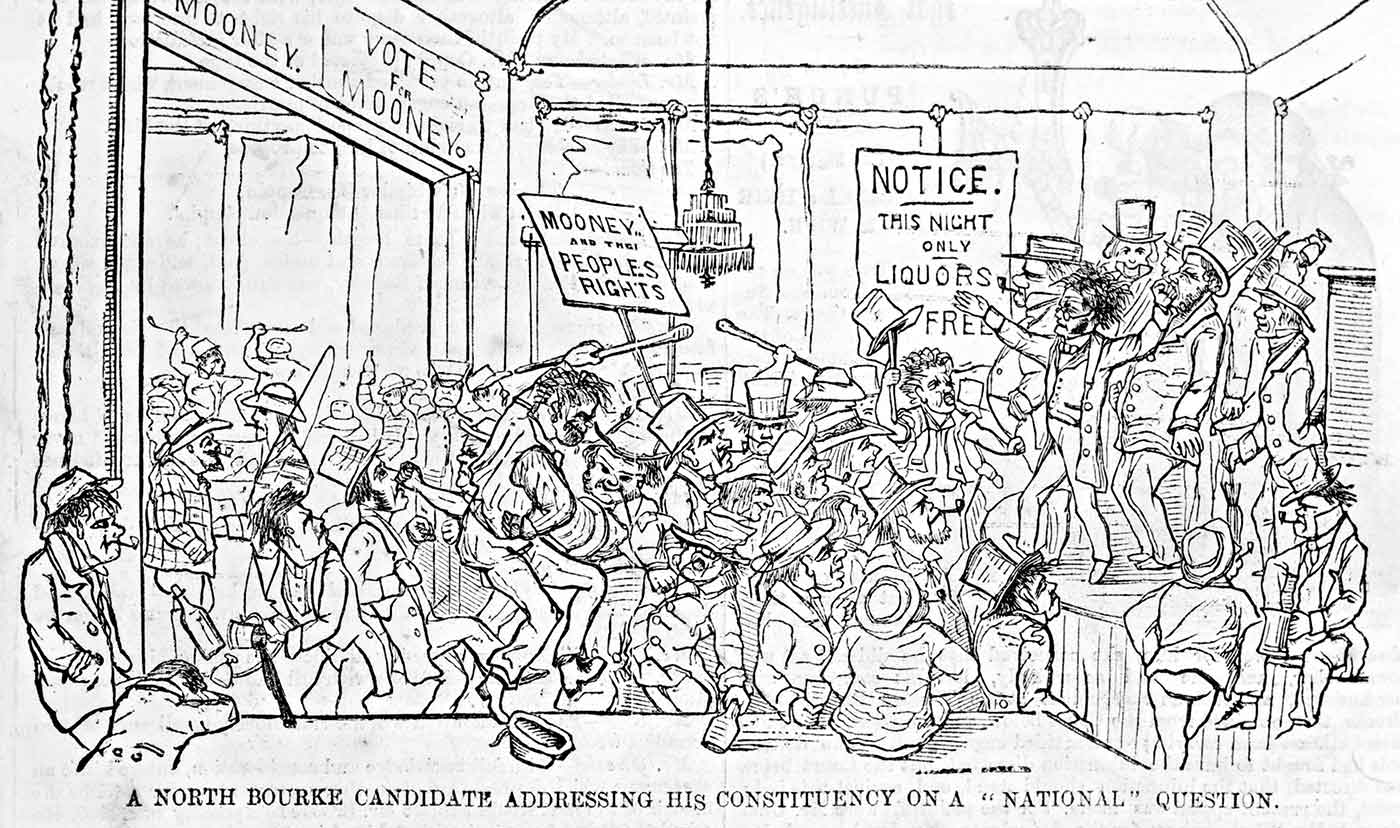
\includegraphics[scale=0.25]{NorthBourke.jpg}
	\caption{Election held in 1855 in Victoria, Australia 
	  was conducted in pub!}
	\end{center}
  \end{figure}   
  


%% Chapters
\chapter{Background}
\label{cha:background}
%At the begging of each chapter, please introduce the motivation and high-level
%picture of the chapter. You also have to introduce sections in the
%chapter. 


\section{Electronic Voting}
   Electronic voting is a nightmare because of a minuscule possibility of 
   bug in software used in voting could lead to a disaster, possibly 
   inverting the results[swisspost]. Given that the cost of 
   electronic voting is 
   so high, we should totally refrain from it; however, on contrary
   it is gaining popularity. Some of the notable countries using some form
   of electronic voting are Estonia (probably the only success story), India,
   Australia, Canada and USA. 
    \begin{figure}[htb]
	\begin{center}
	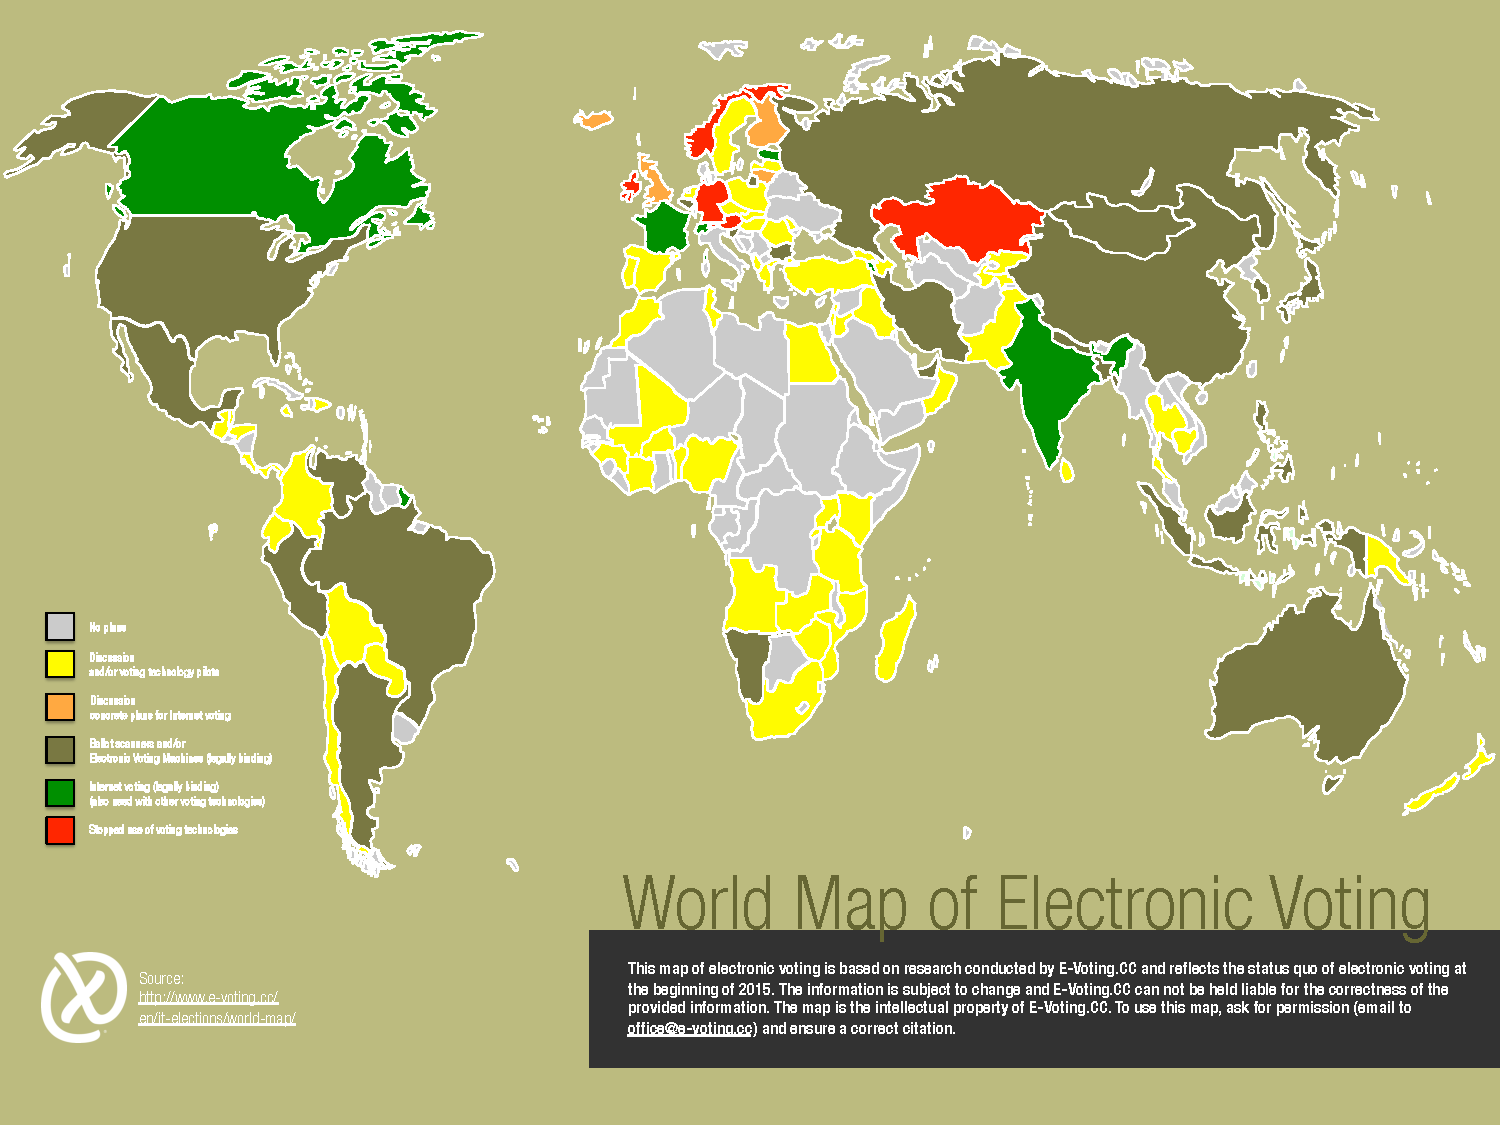
\includegraphics[scale=0.5]{e-voting_worldmap_2015.pdf}
	\caption{World map of Electronic Voting}
	\end{center}
  \end{figure}  
   
  The world can be divided into five categories on 
  parameter of electronic voting\footnote{https://www.e-voting.cc/en/it-elections/world-map}[Figure 2.1]
  \begin{itemize}
  \item No electronic voting (Grey Area)
  \item Discussion and/or voting technology pilots (Yellow Area)
  \item Discussion, concrete plans for Internet voting (Orange Area)
  \item Ballot scanners, Electronic Voting Machines, and Internet Voting
        (Green and Dark Green)
  \item Withdrawn voting technology because of public concern (Red Area)
        Germany, The Nederlands, and UK  
  \end{itemize}    
  
 

   
%  The input method, form of ballot, used the countries participating 
%  in electronic voting can be broadly divided into three group 
  Arguments in favour of electronic voting are 
  increased voter turnout, faster result and cost. Senate 
  election conducted in Western Australia in September 2013 were 
  declared void by high court because of loss of 1370 votes. It was 
  re-conducted in April 2014 with cost of 20 Million AUD with additional 
  delay in results\footnote{https://www.theguardian.com/world/2014/feb/28/western-australia-senate-election-re-run-to-be-held-on-5-april}. Sometimes, 
  the cost is not only concern, but the time involved in counting 
  is. \fix{Give a example of seat which took considerable amount 
  of time in declaring result}. 
  \fix{Add time and cost saving in Indian election after using 
  electronic voting machines} 
  The advantages of electronic voting 
  looks so promising, so why some countries (Red Area) retracted 
  from electronic voting ? Off course, electronic voting makes 
  the process faster, but it has its own layer of added complexities 
  which creates a trust issue among voters. 
  In 2005 German election, two voters filed a case in German 
  Constitutional Court (Bundesverfassungsgericht) because their 
  appeal to scrutinize the elections 
  was not heeded by the Committee. They argued that using electronic 
  voting machines to conduct the election was unconstitutional, and 
  these machines could be hacked, hence results of the 2005 election 
  could not be trusted. The case was argued on the grounds 
  of "all essential steps in the elections are subject to 
  public examinability." according to German Constitution 
  (Basic Law for the Federal Republic of Germany). 
  The Court noted that, under the constitution, elections are 
  required to be public in nature
  
  "The principle of the public nature of elections requires that all 
  essential steps in the elections are subject to public examinability
  unless other constitutional interests justify an exception. 
  Particular significance attaches here to the monitoring of the 
  election act and to the ascertainment of the election result. "
  \footnote{https://www.bundesverfassungsgericht.de/
  SharedDocs/Entscheidungen/EN/2009/03/cs20090303\_2bvc000307en.html}

  The court did not rule out or prevent the usage of electronic 
  voting machines,  but suggested to make the process more 
  transparent and trustworthy.  
  
  "The legislature is not prevented from using electronic voting machines 
  in the elections if the constitutionally required possibility of a 
  reliable correctness check is ensured. In particular, voting machines 
  are conceivable in which the votes are recorded elsewhere in addition
   to electronic storage. This is for instance possible with electronic
   voting machines which print out a visible paper report of the vote 
   cast for the respective voter, in addition to electronic recording 
   of the vote, which can be checked prior to the final ballot and is
    then collected to facilitate subsequent checking. Monitoring that is
     independent of the electronic vote record also remains possible when
     systems are deployed in which the voter marks a voting slip and the 
     election decision is recorded simultaneously, 
     or subsequently by electronic means in 
     order to evaluate these by electronic means at the end of the 
     election day."
  
  The Netherlands were among few countries who adopted electronic voting 
  in early nineties (1990), but it did not go very well long run and was 
  abolished in 2008 
  [http://www.cs.ru.nl/B.Jacobs/PAPERS/E-votingHistory.pdf]. 
  The reason for abolishing electronic voting was that   
  the voting machines used in election were susceptible to many attacks
   and could not stand 
  for public verifiability of results. The decision was victory for 
  Dutch public foundation, Wij vertrouwen stemcomputers niet
  \footnote{English Translation "We do not trust voting computers"}, which 
  demonstrated that e-voting machines used in election leaks enough
  information to guess the option, 
  and they can be easily intercepted from 20 to 30 meters
  \footnote{https://www.youtube.com/watch?v=B05wPomCjEY}. 
  
  
  Germany and The Netherlands are some of the rarest cases where 
  electronic voting was withdrawn because it was not able to 
  replicate the same trust environment as created by paper ballot.
  At this point, the reader can get into the impression that 
  countries who are using electronic voting have successfully 
  created the trust environment in electronic voting. Sadly, 
  it is not the case. India, one of the largest democracy in world, 
  uses electronic voting machines (also known as EVMs) for national 
  and state level 
  elections even though many political parties raised security 
  concern against it.
  It was already shown in 2010 in the paper 
  Security Analysis of India's Electronic Voting Machines by 
  Scott Wolchok et. al 
  [https://jhalderm.com/pub/papers/evm-ccs10.pdf] that it 
  is possible to manipulate the election results by replacing the 
  parts of machine with malicious look alike components with sending 
  them instructions over wireless
  \footnote{https://www.youtube.com/watch?v=ZlCOj1dElDY} 
  \footnote{https://indiaevm.org/}. 
  In recent elections of 2019, the Election Commission of India 
  announced, to ensure the transparency and 
  increase the trust of public, that it would use 
  voter-verified paper audit trail (VVPAT) 
  one per assembly; however, the Supreme Court of India ordered Election 
  Commission of India to increase it to five
  \footnote{https://www.news18.com/news/india/sc-directs-ec-to-increase-vvpat-verification-from-one-evm-to-five-evms-per-constituency-2093363.html}.
  The Commission  would count VVPAT slips 
  in randomly selected one polling booth per assembly 
  constituency in state election and 
  in one polling booth in each assembly segment for national election, but 
  now following the Supreme Court decision it has to do the same for 
  5 randomly selected assembly constituencies/segments. 
  \fix{Find out if there is a document at Election Commission of 
  India website and how the process works}. The design of these 
  machines are closely guard secret,  but it not impossible to gain 
  access as shown by  Scott Wolchok et. al. It would be more 
  interesting and beneficial for Indian democracy if Election 
  Commission of India
  releases the design to public scrutiny (very much like cryptographic
  implementation review process).
  
  
  
 
  
    
  
   
   \subsection{Software Bugs : Origin of Problem}
   
   
   \subsection{Estonia : Success Story}

   \subsection{Universal Verifiability}


\fix{Can I introduce Write Hilbert's idea of mathematical formalism/Frege}

A proof assistant is a computer program which assists users in development of mathematical proofs. The idea of 
developing mathematical proofs using computer goes back to Automath (automating mathematics)
[cite Automath] and LCF [cite Logic for computation] project. The 
Automath project (1967 until the early 80's)  was initiative of De Bruijn, and the aim of the project was to develop
a language for expressing mathematical theories which can be verified by aid of computer.  Automath was first 
practical project to exploit the Curry-Howard isomorphism (proofs-as-programs and formulas-as-types)
 [reference here]. DeBruijn  was likely unaware of this correspondence, and he almost re-invented it 
 ([Wiki entry on Curry-Howard]). Many researchers refers Curry-Howard isomorphism as 
 Curry-Howard-DeBruijn isomorphism. Automath project can be seen as the precursor of
 proof assistants NuPrl [cite here] and Coq [cite coq].   Some other notable  proof assistants are 
 LCF (Logic for Computable Functions)  [cite Milner?], Mizar [cite], Nqthm/ACl2 [cite], PVS [cite], 
 HOL (a family of tools derived from LCF theorem prover), Agda [cite], and Lean [cite].


In this chapter, I will give a overview of theoretical foundation of 
Coq thorem prover i.e. Calculus of Construction and  
Calculus of Inductive Construction, followed by Dependent type 
and how it leads to 
correct by construction (paradigm?) with a example of dependent 
typed lambda calculus. I will also discuss distinction between Type and Prop 
and how it affects the code extraction, a feature for extracting 
certified functional programs from specification proofs, and the 
specification language Gallina. Finally, I would 
argue that why should we trust the Coq proofs even though it does not 
match or look like a mathematical proof.



 
\section{Computer Programming and Type Theory}
	\begin{itemize}
	\item Some tracking of History about how type theory was introduced 
	     to computer programming. Use Dirk's expertise here
	\item Type theory is a logical foundation introduced by 
	      Russel to solve the problem of  paradox in Frege's 
	      Begriffsschrift.
	\item A Church invented formal system of computation, Lambda calculus
	\item A typed lambda calculus
	\item Curry Howard isomorphism
	\end{itemize}


\section{Coq: Interactive Theorem prover}
\label{sec:problemstatement}
\fix{explain here a about Coq. What is Coq ?}
The Coq proof assistant  is an interactive theorem prover based on
underlying theory of Calculus of 
Inductive Construction [Cite Pualine Mohring]  which itself is an 
augmentation of Calculus of Construction 
[cite Huet and Coquand] with inductive data-type.  
 

\subsection{Calculus of Construction}
\subsection{Calculus of Inductive Construction}
\fix{Flesh out the details of 
 Calculus of construction and Inductive construction}
 \fix{Write here about syntax and semantics of CIC}
 
 

 
\subsection{Dependent Types}
    Type system is a wide spectrum ranging from Scheme where 
    type is runtime concept to Haskell to Coq 
    
    \subsubsection{Example : Dependent Type Lambda Calculus}
     Lambda Calculus encoded in Coq using Inductive data type. 
     
 \subsubsection{Correct by Construction}
 \fix{Combing program with proofs leads to one stop solution, mainly 
     correct by construction}
  Well typed program can't go wrong. 
  Give a example of dependent type lambda calculus(Dirk's white board)
  Hello World is dependent type Vector 
 \subsubsection{Program Execution : Proof Certificate}
 \subsubsection{Type vs. Prop : Code Extraction}
 \fix{explain here the difference between Prop and Types. How it affects 
  the code extraction }
  It's good starting point to tell the reader that we have two definitions, 
  one in type and other in prop. Why ? Because Type computes, but it's
  not very intuitive for human inspection while Prop does not compute, 
  but it's very intuitive for human inspection. We have connected that 
  the definition expressed in Type is equivalent to Prop definition. 
 
 \subsubsection{Gallina : The Specification Language}
  The example, dependent type lambda calculus, I gave in previous 
  section was encoded in Coq's specification language Gallina. 
  Gallina is a highly expressive specification 
  language for development of mathematical theories and proving the    
  theorems about these  theories; however, writing proofs in Gallina
  is very tedious and cumbersome. It's not suitable for large proof 
  development, and to ease the proof development Coq also provides 
  tactics.  The user interacting with Coq theorem prover applies these 
  tactics to build the  Gallina term  which otherwise would  
  be very laborious.
  
  \fix{Can I give a simple example to demonstrate the difference 
     between proof build directly in Gallina and proof build using 
     tactics}
  
 
  

 
 \subsection{Trusting Coq proofs}
  The fundamental question for trusting the Coq proofs is two fold: 
  i) is the logic (CIC) sound ?, ii) is the implementation correct ?. 
  The logic has already been reviewed by many peers and proved correct 
  using some meta-logic. The 
  Coq implementation itself can be partitioned into two parts: 
  i) Validity Checker (Small kernel), 
  ii) Tactic language to build the proofs.
  We lay our trust in validity checker, because it's small kernel. If there
  is bug in tactic language which often is the case then build proof would 
  not pass the validity checker.  
  
  Try to write here how Fuzzer failed to find bugs in Compcert. 
  
\section{Summary} 
  Paves the path to Cryptography. 
    
\section{Cryptography}
    Write some basic crypto stuff
    
    \subsection{Homomorphic Encryption}
     Add the details of 
     homomorphic encryption 
     \subsubsection{El-Gamal Encryption Scheme}
        Give both additive and multiplicative
     \subsubsection{Pallier Encryption Scheme}
        Write some description
     \subsection{Commitment Schemes}   
        \subsubsection{Hash Based Commitment Scheme}
        \subsubsection{Discrete Logarithm Based Commitment Scheme}
         Pedersen's Commitment Scheme
     \subsection{Zero Knowledge Proof}
  		Details from 
  	 \subsection{Sigma Protocol : Efficient Zero Knowledge Proof}
  



\section{Summary}











%\label{sec:problemstatement}
Now I give a small example which defines natural number, addition of two natural numbers, and 
proof that addition over natural number is commutative.   We can define 
natural number in Coq using inductive data type (listing 1.1), addition of the natural numbers 
(listing 1.2), and proof that addition of natural numbers is commutative written in Gallina (listing 1.3).

\begin{lstlisting}[language=haskell, numbers=none, basicstyle=\ttfamily, 
caption=Inductive Data Type for Natural Numbers,  captionpos=b, xleftmargin=.1\textwidth]

Inductive Natural : Type :=
 | O : Natural
 | Succ : Natural -> Natural

\end{lstlisting}

More precisely, the interpretation is that Natural is a inductive type with two constructors: i) O representing zero,
and ii) Succ representing successor which takes a Natural number and gives next Natural number.

\fix{Change the Addition into infix symbol + and use + in proofs. It will convey the idea more clearly}
\begin{lstlisting}[language=haskell, numbers=none, basicstyle=\ttfamily,  caption=Addition function for Natural Numbers,  captionpos=b, xleftmargin=.1\textwidth]

 
Fixpoint Addition (n m : Natural) : Natural :=
  match n with
  | O => m
  | Succ n' => Succ (Addition n' m)
  end.

(* Notation for Addition. Now we can use + instead of 
   writing Addition *)
Notation "x + y" := (Addition x y)
            (at level 50, left associativity).
\end{lstlisting}

We define the addition by pattern matching on first argument \textbf{n}. When \textbf{n} is 
O (zero), then we sum is \textbf{m}, and if \textbf{n} is \textbf{Succ n'}, then sum is successor of 
\textbf{n' +  m}.

\begin{lstlisting}[language=haskell, numbers=none, basicstyle=\ttfamily,  caption=Addition function for Natural Numbers,  captionpos=b, xleftmargin=.1\textwidth]

Theorem Addition_by_zero : forall (n : Natural), n + O = n.
  refine (fix IHa (n : Natural) : n + O = n :=
            match n as nz return (nz + O = nz) with
            | O => eq_refl
            | Succ n' =>
              let IHn' := IHa n' in
              eq_ind_r (fun m => Succ m = Succ n') eq_refl IHn'
            end).
Qed.

  
Lemma Successor_addition : forall (n m : Natural),
    Succ (n + m) = n + (Succ m).
  refine
    (fix IHn (n : Natural) : forall m : Natural,
        Succ (n + m) = n + (Succ m) :=
       match n as nz return (forall m : Natural,
                                Succ (nz + m) =
                                nz + (Succ m)) with
       | O => fun m : Natural => eq_refl
       | Succ n' =>
         fun m : Natural =>
           eq_ind (Succ (n' + m))
                  (fun t => Succ (Succ (n' + m)) = Succ t)
                  eq_refl (n' + (Succ m)) (IHn n' m)
       end).
Qed.
     

    
Theorem Addition_is_commutative :
  forall (n m : Natural), n +  m = m + n.
  refine
    (fix IHn (n : Natural) : forall m : Natural,
        n + m = m + n :=
       match n as nz return (forall m : Natural,
                                nz + m =
                                m + nz) with
       | O => fun m : Natural => eq_ind_r (fun t => m = t)
                                      eq_refl
                                      (Addition_by_zero m)
       | Succ n' =>
         fun m  =>
           eq_ind (Succ (m + n'))
                  (fun t => Succ (n' + m) = t)
                  (eq_ind_r (fun t => Succ t = Succ (m + n'))
                            eq_refl (IHn n' m))
                  (m + (Succ n'))
                  (Successor_addition m n')
       end).
Qed.


\end{lstlisting}


We need two additional Lemma:
 i) $Addition\_by\_zero$, a proof of n + 0 = 0,
 and ii) $Successor\_addition$, a proof of Succ (n + m) = n + (Succ m) 
 to prove that addition on Natural is commutative ($Addition\_is\_commutative$), 
 
 One thing that can't escape from the reader's eyes is that the proofs written in Gallina is verbose, and they don't 
 appear anywhere compared to a proof that would have been written by a mathematician. Well, we can lift the burden 
 of verbosity by using tactics provided by Coq; however, there is no universally accepted solution in Coq community 
 for second problem. There has been some research in declarative style proof writing 
 \footnote{www-verimag.imag.fr/~corbinea/ftp/publis/bricks-poster.pdf}, but it is not widely practised in Coq 
 community. The proof of addition on Natural is commutative re-written using tactics (Listing 1.4)
 
 
 \begin{lstlisting}[language=haskell, numbers=none, basicstyle=\ttfamily,  caption=Addition function for Natural Numbers,  captionpos=b, xleftmargin=.1\textwidth]

Lemma Addition_by_zero : forall (n : Natural), n + O = n.
  induction n; cbn; [auto | rewrite IHn; auto].
Qed.


Lemma Successor_addition : forall (n m : Natural),
    Succ (n + m) = n + (Succ m).
Proof.
  induction n; intros m;
    cbn; [auto | rewrite <- IHn; auto].
Qed.


Theorem Addition_is_commutative :
  forall (n m : Natural), n +  m = m + n.
Proof.
  induction n; intro m;
    [rewrite Addition_by_zero |
     rewrite <- Successor_addition;
     rewrite <- IHn]; auto.
Qed.

\end{lstlisting}

Section~\ref{sec:motivation} xxxx.\\


Section~\ref{sec:relatedwork} yyyy.\\


%\section{Motivation}
%\label{sec:motivation}


%\section{Related work}
%\label{sec:relatedwork}
%You may reference other papers. For example: 
%Generational garbage collection~\citep{LH:83,Moon:84,Ungar:84} is perhaps the
%single most important advance in garbage collection since the first collectors
%were developed in the early 1960s. (doi: "doi" should just be the doi part, not
%the full URL, and it will be made to link to dx.doi.org and resolve.
%shortname: gives an optional short name for a conference like PLDI '08.)
%
%
%
%
%
%\section{Summary}
%Summary what you discussed in this chapter, and mention the story in next
%chapter. Readers should roughly understand what your thesis takes about by only reading
%words at the beginning and the end (Summary) of each chapter.




\chapter{Theorem Prover and Cryptography}
\label{cha:theorem_crypto}
 \setlength{\parindent}{2em}
\setlength{\parskip}{1em}

\epigraph{All our knowledge begins with the senses, proceeds then to the understanding, and
 ends with reason. There is nothing higher than reason.} 
{\textit{Immanuel Kant}} 

A proof assistant or theorem prover is a computer program which assists users in development 
of mathematical proofs. Basically, the idea of 
developing mathematical proofs using computer goes back to Automath (automating mathematics)
\citep{deBruijn1983} and LCF \citep{Milner:1972:IAS:942578.807067}. The 
Automath project (1967 until the early 80's)  was initiative of De Bruijn, and the aim of the project was to 
develop a language for expressing mathematical theories which can be verified by aid of computer.  
Moreover, the Automath was first 
practical project to exploit the Curry-Howard isomorphism (proofs-as-programs and formulas-as-types). 
DeBruijn  was likely unaware of this correspondence, and he almost re-invented it.
The Automath project can be seen as the precursor of
 proof assistants NuPrl \citep{Constable:1986:IMN:10510} and Coq \citep{Bertot:2004:ITP}.  
 Some other notable  proof assistants are 
 Nqthm/ACl2 \citep{507872}, PVS \citep{Owre:1992:PPV:648230.752639},
 HOL (a family of tools derived from LCF theorem prover) \citep{Slind:2008:BOH:1459784.1459792}
 \citep{Harrison:1996:HLT:646184.682934} \citep{Nipkow:2002:IHP},
 Agda \citep{Norell:2008:DTP:1813347.1813352}, and Lean \citep{10.1007/978-3-319-21401-6_26}.


\textbf{Chapter overview:}
 This chapter is an overview of the Coq theorem prover and cryptographic primitives. 
 In the Section \ref{sec:problemstatement}, we will give a brief overview of 
 theoretical foundation, calculus of construction and calculus of inductive 
 construction, of Coq.  In the Section \ref{sec:typeprop}, we will discuss
 the difference between \texttt{Type} and \texttt{Prop}
 which is very crucial from program extraction point of view.  The goal of 
 our formalization was not only proving the correctness of 
 Schulze method, but extracting  OCaml/Haskell code to count 
 ballots.  In the Section \ref{sec:deplambda}, we will focus 
 on dependent types and  how it leads to correct by construction paradigm
 by designing a  type safe printf function. 
 Section \ref{sec:gallina} focuses on Coq specification language 
 \texttt{Gallina} with an example showing that why writing proofs using  
 \texttt{Gallina} is difficult and cumbersome, and how it can be eased by 
 using tactics. Finally, in the Section  \ref{sec:coqproof}, we will take 
 philosophical route to justify that why should we trust in Coq proofs 
 even though they do not appear anywhere near to a proof written by 
 a human.  In the Section \ref{sec:cryptography}, we give some historical 
 context and modern day usage of cryptography.  In the following Section 
 \ref{sec:group}, we describe \textit{Group} which is the underlying 
 algebraic structure for Diffie-Hellman construction (\ref{sec:diffie-hellman}). 
 In the next two sections, we describe the ElGamal encryption (\ref{sec:elgamal}) 
 and Homomorphic Encryption (\ref{sec:homomorphic-enc}). In addition, 
 we show the both homomorphic property, multiplicative and additive, 
 of ElGamal encryption. We explain the concept of Zero-Knowledge-Proof 
 and Zero-Knowledge-Proof  of knowledge in Section \ref{sec:zkp}. 
 In the next two sections, we discuss Sigma protocols (\ref{sec:sigma}), 
 an efficient way to achieve zero knowledge proof, and Commitment schemes
 (\ref{sec:commscheme}), a cryptographic protocol to force two mutually 
 distrusting parties to behave honestly with the explanation of Pedersen 
 commitment scheme based on discrete logarithm.  Finally, we give a 
 brief summary pointing to the resources for theorem proving and 
 cryptography. 
 


\section{Coq: Interactive Proof Assistant}
\label{sec:problemstatement}
Coq  is an interactive proof assistant (theorem prover) based on
theory of Calculus of 
Inductive Construction \citep{Paulin-Mohring:1993:IDS:645891.671440} which itself is an 
augmentation of Calculus of Construction 
\citep{Coquand:1988:CC:47724.47725}.  
The underlying theory of CoC and CIC is (typed) lambda calculus, so 
before we describe the CoC and CIC syntax and its typing judgement, 
we will take a brief detour to explain 
different variants of lambda calculus starting from 
untyped lambda calculus and moving up in the ladder by 
adding various abstractions. Later, we will show that 
these all variant, including CoC, can be abstracted into one 
framework by using pure type system \citep{berardi1988towards} 
\citep{Barendregt:1993:LCT:162552.162561}.  
In addition, 
pure type system can be extended with three rules, 
inductive data type, pattern matching, and recursion 
to accommodate Calculus of Inductive Construction.

Lambda calculus was invented by Alonzo Church in the 1930s, 
and his motive was to use lambda calculus as a foundation 
for formal mathematics, specifically the notation of 
computable function by means of an algorithm.  
It is a simplest programming language having just 
three constructs, i.e. variable, application, and abstraction, 
and the abstract syntax tree of lambda calculus is:
\begin{displayquote}

T = V (* Variables *) \\
   | $\lambda$ V. T (* Abstraction *) \\
   | T T       (* Application *)

\end{displayquote}

Using these three rules, we can construct the lambda terms corresponding to 
various mathematical notions. For example, we can represent
$True$ as $\lambda x. \lambda y. x$, $False$ as $\lambda x. \lambda y. y$,
$Zero$ as $\lambda f.\lambda x. x$,  $One$ as $\lambda f.\lambda x. f x$, etc. 
However, there is nothing which is stopping us to construct lambda terms which 
has no apparent meaning, e.g. applying a variable $x$ with itself learning to a lambda 
term $x x$. To avoid these kind of terms, we extend the lambda calculus with 
another abstraction called \textit{types}. Moreover, we add \textit{typing judgement} (rule) 
which dictates which terms is well-typed and which one is not.  This new 
lambda calculus augmented with \textit{types} is known as 
\textit{Simple Typed Lambda Calculus}, represented as $\lambda^{\to}$. 
The abstract syntax tree for \textit{Simple Typed Lambda Calculus} is:

\begin{displayquote}

 
$\mathcal{T} = \mathcal{V} $ (* Type Variable *) \\
                     | $\mathcal{T \rightarrow T}$ (* Arrow Type *)

\end{displayquote}

\begin{displayquote}
T = V (* Variables *) \\
   | $\lambda$ V : $\mathcal{T}$. T (* Abstraction *) \\
   | T T       (* Application *)

\end{displayquote}

\noindent
The typing judgement is a relation between \textit{types} and \textit{terms} in some abstract typing context $\Gamma$. The $\Gamma$ 
is a set/list of typing assumption of the form $x : A$, meaning $x$ is of type $A$. Moreover, $\Gamma$ $\vdash$ $x : A$ means that 
the term $x$ has type $A$ in the context $\Gamma$.
The typing judgement of \textit{Simple Typed Lambda Calculus} 
has three rules, \textit{Var, Abstraction}, and \textit{Application}, to ensure that the terms are well-typed:
\begin{itemize}
\item Var: \[ {\frac {\text{x : A }  \in \text{  }\Gamma }{\Gamma \text{  } \vdash \text{  x : A }} \]
\item Abstraction: \[ {\frac {\Gamma \text{, x : A } \vdash \text{ e : B }}{\Gamma \text{  }\vdash \text{ } (\lambda \text{ x : A. e ) : }A \rightarrow B}} \]
\item Application: \[ {\frac {\Gamma \text{  } \vdash \text{ f : } A \rightarrow B \quad \Gamma \text{  }\vdash \text{ x : A }}{\Gamma \text{  } \vdash \text{  f  x  : B} }} \]
\end{itemize}

\noindent
Now these three typing judgement rules rule out the term $x x$ because it is not well-typed term, and this can be 
inferred from \textit{Application} rule. 
The  \textit{Application} rule states that for $f$ $x$ to be a well typed term of some type $B$, the $f$ has to have 
a type $A \rightarrow B$ for some type $A$ and $x$ has to have the type $A$. Following the 
\textit{Application rule}, for $x x$ to be well typed, the $x$ has to have a arrow type $A \rightarrow B$
and type $A$ in some typing context $\Gamma$. However, it is not possible that $A$ = $A \rightarrow B$
leading to rejection of term $xx$. 

Simple typed lambda calculus is great for many practical purposes except it is verbose. Consider a function 
which takes a input and simply returns it, also known as identity function. Assuming that we two 
base type, $nat$ for the type of natural numbers and $bool$ for type of boolean values, as member of 
type variable set $\mathcal{V}$. We can represent a
 identity function on boolean value as $\lambda x : bool. x$, and on natural number as 
 $\lambda x : nat, x$. In general, we would have one identity function per type. We can 
 abstract these types in to type variable, but we need to type these type variables as well
 to keep everything well typed.  Consequently, abstracting the 
 \textit{types} over type variable, which itself is of sort \textit{kinds} and represented as $*$, 
 leads to \textit{Second Order Lambda Calculus} ($\lambda2$), and 
 now the identity function over different types can be abstracted into a single function:
 $\lambda \alpha : \star. \lambda x : \alpha. x$.
 There are various other variants or abstractions 
 of typed lambda calculus, which we would not discuss here, that can be categorized into:
 \begin{itemize}
 \item Terms depending on terms ($\lambda^{\to}$)
 \item Terms depending on types  ($\lambda2$)
 \item Types depending on types  ($\lambda {\underline{\omega}}$)
 \item Types depending on terms  ($\lambda P$)
 \end{itemize}


% \begin{figure}[!htb]
%        \center{\includegraphics[width=\textwidth]{figs/Lambda_Cube_img.svg.png}}
%        \caption{Lambda Cube}
%      \end{figure} 

All these variation of lambda calculus can be captured into a unified framework
known as \textit{Pure Type System} or \textit{Generalized Type System}.
The \textit{PTS} is group of type system that allows the dependencies between 
types and terms. Unlike the simple typed lambda calculus ($\lambda^{\to}$) where 
terms and types live in two disjoint world, \textit{PTS} blurs this distinction between 
types and terms.  The abstract syntax  of pure type system:
 \begin{displayquote}

    T = V   (* \textit{variable} *)\\
       |  C   (* \textit{constant} *)\\
       | T T (* \textit{application} *)\\
       | $\lambda$ V : T. T (* \textit{abstraction}*) \\
       | $\prod$ V : T. T  (* \textit{dependent function type} *)
   \end{displayquote}

\noindent
The pure type system parametrized by a specification, i.e. 
set of sorts $S$, axioms $A$, and rules $R$, such that: 

 \begin{itemize}
	\item $S$ is a subset of  $C$, i.e.  $S \subseteq C$. 
	\item $A$ is the axioms of form \textit{c : s} where $c \in C$ and $s \in S$, i.e.  $A \subseteq C \times S$. 
	\item $R$ is the set of rules of form $(s_{1}, s_{2}, s_{3})$ such that $s_{1}, s_{2}, \text{ and } s_{3} \in S$, i.e.
	 $R \subseteq S \times S \times S$.
 
 \end{itemize}
 
\noindent 
The typing judgement for \textit{PTS} in typing context $\Gamma$ is defined by following rules ($s$ ranges of $S$, and $x$ ranges over V 
 with usual notion of  variable capture avoidance):
 \begin{itemize}
 \item Axiom: \[ \frac{\text{c : s } \in A}{\Gamma \text{  } \vdash \text{ c : s}} \]
 \item Start: \[ \frac{\Gamma \text{  } \vdash \text{ A : s}}{\Gamma \text{, x : A }\vdash \text{ x : A}} \]
 \item Weakening: \[ \frac{\Gamma \text{ } \vdash \text{ A : B } \quad \Gamma \text{ } \vdash \text{ C : s }}{\Gamma, \text{ x : C } \vdash \text{ A : B }} \]
 \item Product: \[ \frac{\Gamma \text{ } \vdash \text{ A : }s_{1} \quad \Gamma, \text{ x : A } \vdash \text{ B : }s_{2}}{\Gamma \text{ } \vdash (\prod \text{ x : A. B) : }s_{3}} \]
 \item Application: \[ \frac{\Gamma \text{ }\vdash \text{ F : (}\prod \text{x : A. B)} \quad \Gamma \text{ }\vdash \text{ a : A }}{\Gamma \text{ }\vdash \text{ F a : B [x := a]}} \]
 \item Abstraction: \[ \frac{\Gamma, \text{ x : A }\vdash \text{ b : B } \quad \Gamma \text{ }\vdash (\prod \text{x : A. B) : s }}{\Gamma \text{ }\vdash (\lambda \text{x : A. b) : (}\prod \text{ x : A. B)}} \]
 \item Conversion: \[ \frac{\Gamma \text{ }\vdash \text{ A : B } \quad \Gamma \text{ }\vdash \text{ B' : s } \quad \text{B  }=_{\beta} \text{ B' }}{\Gamma \text{ } \vdash \text{ A : B' }} \]
\end{itemize}   



\subsection{Calculus of Construction/Inductive Construction}
\label{sec:cc}
The Calculus of Construction is a higher order  natural deduction style proof system 
for constructive proofs where every proof a typed $\lambda$-abstractions.  Using the 
\textit{Pure Type System} syntax, it can be expressed as:

\begin{displayquote}

    $S$ = \[ \lbrace  Prop \rbrace \cup \lbrace  Type_{i} \mid  i \in \mathbb{N} \rbrace \]
    $A$ =  \[ \lbrace Prop : Type_{0} \rbrace \cup \lbrace Type_{i} : Type_{i+1} \mid i \in \mathbb{N} \rbrace \]
    $R$ = 
     \[
   \left\{ \begin{array}{l}
   (Prop, Type_{i}, Type_{i}) \text{      } i \in \mathbb{N}  \\
   (s, Prop, Prop)  \text{     } s \in S \\
   (Type_{i}, Type_{j}, Type_{max (i, j)}) 
  \end{array}\right\}
\]
       
\end{displayquote}

\noindent
The sort \textit{Prop} captures type of expression which represents logical proposition, while 
the sort \textit{Type} captures the computational content.   Calculus of Construction is
 powerful enough to encode inductive definitions \citep{pfenning1989inductively}, but 
 one of the main drawback is efficiency of computation of function over these encoded 
 inductive definitions, and some other properties could not be proven \citep{10.1007/3-540-45413-6_16}.
In order to solve these problems, \citep{Paulin-Mohring:1993:IDS:645891.671440}  introduced 
Inductive definitions, pattern matching, and fixpoint in the Calculus of Construction to make the data structure 
representation more efficient. Below is the  (incomplete) syntax of Calculus of Inductive Construction:

 \begin{displayquote}

    T = ...  (*  Pure Type System *) \\
       | Ind $\lbrace$ V : T :=  $\textbf{V : T} \rbrace$.V (* inductive definition) \\
       | case T of \textbf{V => T} (* pattern matching *)  \\
       | fix_{n}  $\lbrace$ V : T := T $\rbrace$ (* recursion *) \\
   \end{displayquote}
 

\noindent 
\textit{Inductive Type:} As we mentioned above that inductive types are basic building block for encoding various 
data structures in the Coq (CIC). The keyword to declare a inductive data type in Coq is 
\textit{Inductive}. For example, a length index list
whose elements belong to a type $A$ can defined as (also known as vector):

\begin{minted}{coq}

Inductive Vector (A : Type) : nat -> Type :=
| Nil : Vector A 0
| Cons n : A -> Vector A n -> Vector A (S n).

\end{minted}

\noindent 
Now we can define various functions for the \textit{Vector} data structure. For example, 
we can define a function to append two vectors for length $n$ and $p$ as:

\begin{minted}{coq}
Fixpoint append {A n p} (v : Vector A n) (w : Vector A p)  
  : Vector A (n + p) :=
  match v with
  | Nil _ => w
  | Cons _ _ a v' => Cons _ _ a (append v' w)
  end.

\end{minted}
 
\noindent
The expressiveness of Coq allows to encode various correctness properties at type level. 
In our example of \textit{append}, the correctness criteria states that appending a 
vector of length $n$ with a vector of length $p$ yields a vector of length $(n + p)$.  
In other words, the function \textit{append} is "correct-by-construction". 
During our formalisation, we have encoded our vote counting 
as a \textit{Inductive} data type with various assertions of 
correctness criterion appearing at type level. These assertions at type level 
enforce that only the "correct" term of vote counting inductive data type can be constructed
(\textit{correct-by-construction}).



We would like to point that the current underlying theory of Coq has been 
extended with Co-Inductive types \citep{10.1007/3-540-60579-7_3}; however, 
the discussion of Co-Inductive types is not very relevant for this thesis.	

 
\subsection{Type vs. Prop: Code Extraction}
\label{sec:typeprop}
 Every term in Coq has
 a type, and the term could be either a logical proposition 
 or computational term. 
 The type of logical propositions are \textit{Prop}, while the type of 
 computational parts are \textit{Type}. This distinction between 
 the type of logical propositions (Prop) and the type of computational 
 parts  (Type) provides a mechanism to extract 
 functional programs directly from Coq proof scripts.
 During the extraction process \citep{Letouzey:2008:ECO}, 
 every term of type Prop is removed and no longer exists in extracted 
 code, and only the terms of type Type are translated into target language
 (OCaml/Haskell/Scheme). Because of this, Coq in general does not allow
 the case analysis on
 the terms (logical objects) of sort Prop   when the goal is in not in Prop,
 but in certain cases it can be achieved (we call this special 
 case reification and explained next). 
 
 
  
  \subsubsection{Reification}
  \label{sec:reification}
  Sometimes it is very natural to express certain properties/definitions
  in the Prop than the Type. Moreover, the definitions/terms in the Prop are self contained and 
  very intuitive for human understanding. The only problem is that the terms of the type Prop do not carry any 
  computational content but only the proof part. However, 
  we can escape this situation if the term of type Prop is decidable predicate (boolean predicate) and its domain is finite. 
  In the case of decidable predicate in Prop over a finite domain,  we can extract 
  the witness constructively by using 
  a program of linear search that tries the decidable predicate on 
  every element of its (finite) domain. Below is the linear search 
  reification code 
  which produces a Type level witness, \textit{existsT},
  from a Prop level witness, \textit{exists}, by iterating 
  through all the elements of finite type $A$ (the finiteness 
  of $A$ is captured by the list $l$).
  
  
  
\begin{minted}{coq}
Require Import Coq.Lists.List.
Import ListNotations.

(* type level existential quantifier *)
Notation "'existsT' x .. y , p" :=
  (sigT (fun x => .. (sigT (fun y => p)) ..))
    (at level 200, x binder, right associativity,
     format "'[' 'existsT'  '/  ' x  ..  y ,  '/  ' p ']'")
  : type_scope.

(* the following shows that a decidable (or boolean valued) 
   predicate on a finite list
   can always be reified in terms of strong existence *)
Theorem reify {A: Type} (P: A -> bool) : forall (l: list A), 
    (exists x, In x l /\ P x = true) -> existsT x, P x = true.
Proof.
  refine (
      fix Fn l :=
        match l with
        | [] => fun H => _
        | h :: tl => fun H => _
        end).
  contradict H. intro.
  destruct H as [x [H1 H2]].
  firstorder.

  assert (Hbiv: {P h  = true} + {P h <> true}).
  decide equality.
  destruct Hbiv as [Htrue | Hfalse].
  exists h. assumption.
  specialize (Fn tl). apply Fn.
  destruct H as [x [H1 H2]].
  destruct H1. subst.
  firstorder. exists x.
  firstorder.
Defined. 

\end{minted}
    
    
    
  We have used many standard tricks like this  
  to make  our formalization more accessible for human inspection.
  For example, we have two definition, one in Prop and other in Type, 
  of winner, loser and path. The rationale behind two definitions 
  is that that Prop definitions are very natural and easy to understand 
  compared to their Type counter part. Furthermore, we have shown that they are 
  equivalent to each other, and used the definitions in Type for
  computation.  Also, there is a nice Coq library 
  ConstructiveEpsilon\footnote{https://coq.github.io/doc/master/stdlib/Coq.Logic.ConstructiveEpsilon.html}
  which uses the similar trick as ours; however, we have not used this library in 
  our formalization. 
 \subsection{Correct by Construction: Type Safe Printf}
 \label{sec:deplambda}
  One of the highly sought feature of Coq is dependent type, 
  a type which is parametrised by value.  
  The expressiveness of dependent type make it possible
  to express specification at type level, and these specifications enables larger 
  set of  logical errors to eliminated at compile time. 
  
 
 Using the expressiveness of dependent type, we construct a type-safe version of 
 printf \citep{Pierce:2004:ATT:1076265}. Our goal is to generate compiler error when the given format string and the type of 
 corresponding input values  
 do not match, e.g. printf "\%d \%s" "hello Coq" 42 should be compiler error because
 \%d is a directive for integer value, but the type of input, "hello Coq", is string. In addition, 
 type-safe printf should print the input when the format string is aligned with type of input, e.g.
 printf "\%s \%d" "hello Coq" 42 should print the string "hello Coq  42" because the first directive 
 of format string, \%s, and type of input, "hello Coq", are aligned. Similarly, the second directive 
 of format string, \%d, is also aligned with the type of input, 42.
 
 The high level idea is to split the printf arguments into two parts: i) format string, 
 and ii) values to be printed. For example, printf "\%s \%d" "hello Coq" 42 would be split into "\%s \%d", and 
 "hello Coq" 42.  Based on the format string, we design two functions: i) a type level function, 
 and ii) a value level function. The type level function would 
 take format string and returns a variadic function type, e.g. 
 on format string "\%s \%d", it would return a function type with 
 signature \texttt{string -> Z  -> string}.
 The value level function, whose type signature 
 is constructed by the type level function, would take the values to printed as input. If the 
 type of values to be printed is aligned with the type constructed by the type level function then 
 we proceed to print the string, otherwise we generate compiler error.  
 


First, we defined a abstract syntax tree, \textit{format}, to make it explicit the characters we 
are interested in format string. Additionally, the \textit{format\_string} function takes the format string 
and returns the abstract syntax tree, and the type level, \textit{interp\_format}, takes the 
abstract syntax tree and returns the function type corresponding to format string.

\begin{minted}{coq}
(* abstract syntax tree *)
Inductive format :=
| Fend : format
| Fint : format -> format
| Fstring : format -> format
| Fother : ascii -> format -> format.

(* turn the format string into abstract syntax tree *)
Fixpoint format_string (inp : string) : format :=
  match inp with
  | EmptyString => Fend
  | String ("%"%char) (String ("d"%char) rest) => 
        Fint (format_string rest)
  | String ("%"%char) (String ("s"%char) rest) => 
       Fstring (format_string rest)
  | String c rest => Fother c (format_string rest)
  end.


(* construct the type level function from abstract syntax tree *)
Fixpoint interp_format (f : format) : Type :=
  match f with
  | Fint f => Z  -> interp_format f
  | Fstring f => string -> interp_format f
  | Fother c f => interp_format f
  | Fend => string
  end.
\end{minted}


\noindent
The \textit{interp\_format} function returns a function type 
(\texttt{Z -> string -> string -> string})  on the (abstract syntax tree of) 
format string "\%d \%s \%s" 

\begin{minted}{coq}
Eval compute in interp_format (format_string "%d %s %s").
(* = Z -> string -> string -> string
     : Type *)
\end{minted}

Now, we construct a value level function, \textit{interp\_value}, whose type 
is constructed by type level function, and it will take the values to be printed as input.
The type of values to print should match the type constructed by type level 
function for successful type checking otherwise it will be type error. 

\begin{minted}{coq}
(* value level function whose type is constructed 
    on fly by interp_format function *)
Fixpoint interp_value (f : format) (acc : string) : 
  interp_format f :=
  match f with
  | Fint f' => fun i => interp_value f' (acc ++ of_Z i)
  | Fstring f' => fun i => interp_value f' (acc ++ i)
  | Fother c f' => interp_value f' (acc ++ String c EmptyString)
  | Fend => acc
  end.
\end{minted}

\noindent
Finally, we define the printf function, and evaluate it on two inputs: 
i)  printf "\%d \%s" "hello Coq" 42, and ii)  printf "\%d \%s" 42 "hello Coq".

\begin{minted}{coq}
Definition printf s := interp_value (format_string s) "".           

Eval compute in  printf "\%d \%s" "hello Coq"%string 42.
(* Error: The term ""hello Coq"%string" has type "string" 
while it is expected to have type "Z". *)

Eval compute in  printf "\%d \%s" 42 "hello Coq"%string. 
(*  "\0b101010 \hello Coq"%string. The number 
42 is printed in binary *)                            
\end{minted}
The first input, printf "\%d \%s" "hello Coq" 42, is type error because 
printf "\%d \%s" returns a value level function whose  type is Z -> string -> string, but 
the type of first argument, "hello Coq", is string which does not unifies with Z,
while second one is successfully printed as string. 

  
  

 
 \subsection{Gallina: The Specification Language}
 \label{sec:gallina}
  The example, type safe printf function, I gave in previous 
  section was encoded in Coq's specification language Gallina. 
  Gallina is a highly expressive specification 
  language for development of mathematical theories and proving the    
  theorems about these  theories; however, writing proofs in Gallina
  is very tedious and cumbersome. Furthermore, It is not suitable for large proof 
  development. In order to ease the proof development, Coq also provides 
  tactics.  The user interacting with Coq theorem prover applies these 
  tactics to build the  Gallina term  which otherwise would  
  be very laborious.
  
 We have written two proofs that addition on natural number is commutative. 
 First proof, \textit{addition\_commutative\_gallina}, is written using 
 Gallina, while the second proof, \textit{addition\_commutative\_tactics}, is written 
 using the tactics.  In general, we write programs directly in Gallina and use tactics 
 to prove properties about the programs. However, there is no fixed set of rules, and tactics 
 can be used to write programs with dependent types (which we have done during this
 formalization).
 
\begin{minted}{coq}
(* proof written using Gallina *)
Lemma addition_commutative_gallina : 
    forall (n m : nat), n + m = m + n.
refine
      (fix Fn (n : nat) : forall m : nat, n + m = m + n :=
        match n as n0 
              return (forall m : nat, n0 + m = m + n0) with
        | 0 => fun m : nat => 
           eq_ind_r (fun n0 : nat => m = n0) 
                     	eq_refl (Nat.add_0_r m)
        | S n' =>
          fun m : nat =>
            eq_ind_r (fun n0 : nat => S n0 = m + S n')
                     (eq_ind_r (fun n0 : nat => S (m + n') = n0) 
                     eq_refl (Nat.add_succ_r m n')) (Fn n' m)
        end).
Qed.

(* proof written using tactics *)
Lemma addition_commutative_tactics :
  forall (n m : nat), n + m = m + n.
  intros n m; try omega.
Qed.
\end{minted}



 \subsection{Trusting Coq proofs}
 \label{sec:coqproof}
  In general, Coq proofs are nowhere similar to a mathematical 
  proof written by trained mathematician. Also, these proofs 
  are verbose and fairly long, so a 
  very fundamental question is: why should we 
  accept or believe in a proof written in Coq \citep{pollack1998believe}?  Generally, the answer of 
	accepting or trusting Coq proos is two fold:
  i) is the logic (CIC) sound?, and ii) is the implementation correct?
  The logic has already been reviewed by many peers and proved correct 
  using some meta-logic, therefore the answer of our question about trusting Coq proof 
  hinges on the implementation. 
  The Coq implementation (written in OCaml)  has two parts, the type checker (small kernel), 
  and tactic language to build the proofs.
  We lay our trust in type checker, because it is a small kernel and can be 
  manually inspected. Furthermore, if there
  is a bug in tactic language, which often is the case, then build proof would 
  not pass the type checker.  Also, we can use the publicly available proof 
  checkers written by experts and inspected by many others. In addition, to increase the 
  confidence, there have been 
  efforts to certify type checker \citep{Appel2003}
  \citep{barras1996coq}, verifying meta theory of one proof system 
  in other \citep{10.1007/978-3-319-08970-6_3}, self certificate of 
  theorem prover \citep{10.1007/11814771_17}. However, no system can 
  prove its own consistency (G{\"o}del's second incompleteness theorem), therefore
  trusting human judgement is inevitable.
  
 
\section{Cryptography}
\label{sec:cryptography}
    The word cryptography comes from the two Greek words: 
    \textit{krypt\'{o}s}, meaning \textit{hidden}, and \textit{gr\'{a}fein} meaning \textit{to write}. As a matter of 
    fact, in the past, hidden writing (cryptography), using the symbol replacement, has been used 
    to conceal the message. For example,
    the earliest known usage of cryptography (symbol replacement) goes back to  ancient 
    Egyptian (Khnumhotep {\rm II}, 1500 BCE); however, the purpose of replacing one symbol by other 
    was not to protect
    any sensitive information but to enhance the linguistic appeal. The first known usage of 
    cryptography to conceal the sensitive information goes back Mesopotamians (1500 BCE) where 
    they used it to hide the formula for pottery glaze. Fast forward, around 100 BCE, 
    Julius Caesar wrote a letter to Marcus  Cicero using a method, now known 
    as \textit{Caesar cipher}, which would shift each character in letter by 3 position right with wrapping 
    around, i.e. X would wrap A, Y would wrap to B, and Z would wrap to C. Decryption was 
	3 character left shift.  Using the  tools of modern mathematics, encryption and decryption 
	in \textit{Caesar cipher} is modular addition and modular subtraction (modulo 26), respectively.  
    Overall, cryptography is art and science of making thing  unintelligible from everyone, except the 
    intended recipient.  	
	    
	The modern day cryptography originated in 1970 with two ingenious ideas, \textit{Data Encryption Standard (DES)}, 
	and \textit{Diffie-Hellman Algorithm}. Data Encryption Standard, developed at IBM in 1970, is a symmetric 
	key encryption algorithm which uses the same key for encryption and decryption. Since its inception, Data Encryption Standard
	amassed a bad reputation because of \textit{National Security Agency (NSA)} involvement; however, it had a 
	practicality issue: key management. If the two parties wanted to communicate
	securely over insecure channel using  the Data Encryption Standard, then they needed to agree on a common key. 
	In order to agree on the common key, they needed a secure channel where they can securely communicate the key. 
    The solution to this problem came from \textit{Diffie-Hellman} key exchange where two parties can exchange the 
    key securely over insecure channel. Moreover, the advent of \textit{Diffie-Hellman} key exchange started the 
    whole new area of public key cryptography where encryption and decryption key are different. 
    Although \textit{Diffie-Hellman} key exchange suffers from  man-in-the-middle (MITM)  attack if used for keys exchange in its 
    naivety, e.g. Logjam \citep{Adrian:2015:IFS:2810103.2813707}. Nonetheless, 
    it is a building block ElGamal Encryption \citep{elgamal1985public}. 
    
    
    
    In this thesis, we are mostly concern about public key cryptography.
    The basic working principles of modern day cryptography is based on 
    mathematical principle than vanilla symbol replacement. 
    In addition, it is no longer just 
    used to achieving confidentiality, but various other things, e.g. integrity,  authentication, non-repudiation 
    protocol, digital signature, digital cash, etc.
    These mathematical principle involves 
    various algebraic structures and algorithm to manipulate the object from these structures.
    For example, the underlying mathematical principal of \textit{Diffie-Hellman}  algorithm 
    is hardness of computing discrete logarithms in finite fields.
    
    
  
    
    Now we  describe the workings of Diffie-Hellman \citep{Diffie:2006:NDC:2263321.2269104}
    algorithm, because all the constructions we have used  are based on Diffie-Hellman construction. 
    Before we describe the algorithm, we briefly sketch the algebraic structure Group because it is underlying algebraic structure of 
    Diffie-Hellman  construction  (typically, the underlying 
    structure is multiplicative group of a finite field). Also, note that our definition is influenced theorem-provers/type-theory because 
    we have  written the type signature of group operator $*$ and inverse operator $inv$. 
    
    \subsection{Group}
    \label{sec:group}
    A group is a set $G$, with a binary operator $* : G \rightarrow G \rightarrow G$, identity element $e$, and inverse operator $inv : G \rightarrow G$ such 
    that the following laws hold: 
    \begin{itemize}
     \item \texttt{Associativity}: $\forall$  a b c $\in G,$  $a * (b * c) = (a * b) * c$
    \item \texttt{Closure}: $\forall$ a b $\in G,$  $a * b \in G$
    \item \texttt{Inverse Element}: $\forall$ a $\in G$ $\exists$ $a^{-1} \in G$, such that $a * a^{-1} = a^{-1} * a = e$. $a^{-1}$ is called inverse of a (
     $inv$ $a$).
    \item \texttt{Identity}: $\forall$ a $\in G,$  $a * e = e * a  = a$
    \end{itemize}
   
    \noindent
    Furthermore, if a group is commutative, i.e. 
    $\forall$ a b $\in  G,$  $a * b = b * a$, then we call it abelian group (in honour of Niels Henrik Abel). In addition, 
    if a \textit{group} is \textit{cyclic group} if it can be generated by a single element, also known as generator of group 
    and denoted as $g$, by repeatedly applying the group operator $*$ to itself. Moreover, a group is \textit{finite cyclic group}
    if it is cyclic and the cardinality of the underlying set (carrier set) $G$ is finite. The cardinality is also known as order of group. 
	    
    
     
     \subsection{Diffie-Hellman Construction}
     \label{sec:diffie-hellman}
     	Now we explain \texttt{Diffie-Hellman} construction. The construction can be divided into two steps:
		\begin{enumerate}
		\item The two communicating parties, say Alice and Bob, agree with shared public parameters which 
		are finite cyclic group $G$ of order $p$ ($p$ is a large prime) and generator element $g$.
		\item After agreeing with public parameters, Alice and Bob initiates the key exchange protocol (assuming that 
		 Alice goes first):
		 \begin{enumerate}
		   \item Alice selects a random number $a$, where 1 < $a$ < $p$, computes $g^{a}$ ( $g * g * g ... * g$  $a$ times), and shares 
		   $g^{a}$ with Bob. 
		   \item Similarly, Bob selects are random number $b$, where 1 < $b$ < $p$, computes $g^{b}$, and shares  $g^{b}$
		   with Alice.
		   \item Finally, Alice computes the key $(g^{b})^{a}$, and Bob computes the key $(g^{a})^{b}$.  A basic 
		   algebraic simplification on Alice's key and Bob's key would show that they both have the 
		   common key  $g^{ab}$.
		   
		 \end{enumerate}
      \end{enumerate}		
      
     
      \noindent
       During the whole process, Eve, the adversary, would have $g^{a}$ and $g^{b}$, but she can not compute the 
      $ g^{ab}$ from these two values assuming that discrete logarithm is hard to compute. 
      There are, off course, other attacks exists, e.g. denial of man in the middle attack, Logjam, etc. 
      The security property of \texttt{Diffie-Hellman} construction is formalized using complexity theoretic notion 
      given below (we would not go into the details of complexity theoretic notions):
      
     
      \textbf{DL - Discrete Logarithm problem:} 
      An instance of \textit{DL} problem states that given a finite cyclic group $G$, a generator of $g$ of $G$, and 
      an element $y$, finding an element $x \in G$ such that $g^{x} = y$.
      
      
      \textbf{DH - Diffie-Hellman problem:}
      An instance of \textit{DH} problem   
      states that given a finite cyclic group $G$, a generator of $g$ of $G$, 
      elements $g^{a}$ and $g^{b}$, finding the element $g^{ab}$.
      
      
      \textbf{DDH - Decision Diffie-Hellman Problem:}
      An instance of \textit{DDH} problem states that given a finite cyclic group $G$, a generator of $g$ of $G$,
      elements $g^{a}$, $g^{b}$, and $g^{c}$, determining if $c = a * b$.
      
           	 
     
     \subsection{El-Gamal Encryption Scheme}
     \label{sec:elgamal}
     In 1985, Tahir El-Gamal \citep{elgamal1985public} proposed a new encryption system which was based on Diffie-Hellman algorithm. 
     \textit{El-Gamal} turned the interactive  Diffie-Hellman algorithm into a non-interactive, no need for any active second party, by introducing 
     a randomness.  The \textit{ElGamal} scheme has three phases:
     \begin{enumerate}
		\item \textbf{Key Generation:}   
		The user, say Alice, first chooses a finite-cyclic group $G$ of order $p$ ($p$ is a large prime) and a group group generator $g$.
		She randomly selects a an element $x$ from $\{1, \ldots, p-1\}$ as a private key, computes her public key $h = g^{x}$. 
		Subsequently, she publishes 
		the <$G$, $g$, $p$, $h$> and keeps $x$ private. 
		\item \textbf{Encryption:}
		If any party, say Bob, wants to send a encrypted message $m$ to Alice, then he would randomly select an element 
		r, where 1 < r < p, computes $c_{1} := g^{r}$ and $c_{2} := m * h^{r}$, and send the pair ($c_{1}, c_{2}$) to 
		Alice. 
		\item \textbf{Decryption:}
		Upon receiving any pair ($c_{1}, c_{2}$), Alice would compute $c_{2} * c_{1}^{-x}$. A basic simplification of $c_{2} * c_{1}^{-x}$
		shows that it recovers the plaintext message. The simplification proceeds by replacing the $c_{2}$ with 
		$m*h^{r}$ and $c_{1}$ with $g^{r}$ in $c_{2} * c_{1}^{-x}$. This substitution leads to 
		$m * h ^ {r} * g^{-rx}$ which upon further simplification by replacing the $h$ with $g^{x}$
		leads to $m * g^{xr} * g^{-rx}$. Using the same base rule, the term $m * g^{xr} * g^{-rx}$ can be 
		written as $m * g^{xr - rx}$. Since $x  r = r x$, so we 
		can replace $m * g^{xr - rx}$ with $m * g^{0}$. The term $g^{0}$  = $e$ (the identity of group $G$) and using 
		the right identity group law, we can replace $m * e$ by $m$. 
		
	\end{enumerate}	
    
    \subsection{Homomorphic Encryption}
    \label{sec:homomorphic-enc}
	 Homomorphic encryption  is a encryption scheme which allows us to perform useful operation on 
	     encrypted data without decrypting the data.
	     It was first posed by Rivest, Adleman and Dertouzos in \citep{rivest1978data}: 
      
       \begin{displayquote}  
	     Consider a small loan company which uses a commercial time-sharing service to store its records.  
	     The loan company’s "data bank" obviously contains sensitive information which should be kept private.  
	     On the other hand, suppose that the information protection techniques employed by the time sharing 
	     service are not considered adequate by the loan company.  In particular, the systems programmers would 
	     presumably have access to the sensitive information.  The loan company therefore decides to encrypt all 
	     of its data kept in the data bank and to maintain a policy of only decrypting data at the home office -- data 
	     will never be decrypted by the time-shared computer.
	   \end{displayquote}  

 \noindent	     
 A encryption scheme is homomorphic if for any two plaintext $x$ and $y$:
		\begin{displayquote}
		
		 $Enc_{pk}(x) \bigotimes Enc_{pk}(y) = Enc_{pk} (x \bigoplus y)$  where 
		$Enc$ is encryption function, $pk$ is the public key, $\bigotimes$ is operation on ciphertext, and $\bigoplus$
		 is operation on plaintext.
		
		\end{displayquote}
				
		These two operators $\bigotimes$ and $\bigoplus$ are very specific. If a cryptosystem that supports an arbitrary 
		function $f$ on ciphertext, then it is called fully homomorphic cryptosystem:
		\begin{displayquote}
		  $ f (Enc_{pk}(m_{1}), Enc_{pk}(m_{2}), ..., Enc_[pk}(m_{k}) = Enc_{pk}( f (m_{1}, m_{2}, ..., m_{k}))$ 
	    \end{displayquote}
		
		\noindent
		The first fully homomorphic encryption system was proposed by Craig Gentry \citep{Gentry:2009:FHE:1834954}; however, 
		in this thesis we are mostly concern with partially homomorphic encryption (either additive or multiplicative, but not both),
		specifically additive ElGamal, 
		so we are not going to present the details overview 
		of Craig Gentry fully homomorphic construction. From now on, we would be using the term homomorphic encryption for 
		partially homomorphic encryption. 
		 	    
	    
	    
	    
	     
	    Now, keeping in mind that homomorphic encryption enables us to perform useful operation on encrypted data, 
	    we will see what kind of homomorphic property is exhibited by the ElGamal method discussed in the previous section. 
	    Given a public infrastructure <$G, p, g, h$> for ElGamal scheme, 
	     we encrypt two message $m_{1}$ and $m_{2}$ by taking two random numbers $r_{1}$,  $r_{2}$ from the group:
	     \begin{displayquote}
	     $Enc(m_{1}, r_{1}) := (g^{r_{1}}, m_{1} *  h^{r_{1}})$ 
	      \end{displayquote}
	     
	     \begin{displayquote}
	     $Enc(m_{2}, r_{2}) := (g^{r_{2}}, m_{2} *  h^{r_{2}})$ 
	      \end{displayquote}
	     
	     
	     If we mutiply these two cipher together pairwise, we get ($g^{r_{1}+ r_{2}}, m_{1} * m_{2} *  h^{r_{1} + r_{2}}$). 
	     After decrypting this combined ciphertext, we will get $m_{1} * m_{2}$. In the scheme, $\bigotimes$ is multiplication and 
	     $\bigoplus$ is also multiplication. Furthermore,  
	     if our end goal is  to achieve multiplication on a bunch of plaintext, then rather than decrypting the corresponding ciphertext individually 
	     and multiplying them, we could simply multiply all the ciphertext together and decrypt the final result.  
	     The advantage of this scheme is that it does not leak the individual values which, sometimes, is a very crucial property in many 
	     application, specifically election voting.
	     In electronic voting protocols, we do not want to reveal the choices of a individual voter, but it is acceptable to reveal the final tally. 
	     However, this scheme is not suitable for electronic voting schemes because it is multiplicative. Almost, to the best of 
	     my knowledge, all the electronic voting scheme calculate the finally tally by adding the individual choices of all
	     voters, so the requirement is achieve the addition on plaintext. 
	     There are 
	     many additive homomorphic encryption schemes, e.g. Benaloh cryptosystem, Paillier cryptosystem, etc. In addition, we 
	     can modify the ElGamal encryption scheme to make additive. In additive case, it works as:
	       \begin{displayquote}
	      $Enc(m_{1}, r_{1}) := (g^{r_{1}}, g^{m_{1}} *  h^{r_{1}})$ 
	      \end{displayquote}
	     
	     \begin{displayquote}
	    $Enc(m_{2}, r_{2}) := (g^{r_{2}}, g^{m_{2}} *  h^{r_{2}})$ 
	      \end{displayquote} 
	     
	    
	     
	    
	      \noindent
	      Multiplying these two ciphers pairwise would give us,  ($g^{r_{1} + r_{2}}$, $g^{m_{1} + m_{2}} * h^{r_{1} + r_{2}}$) which would decrypt as 
	      $g^{m_{1} + m_{2}}$. In this case, $\bigtimes$ is multiplication and $\bigoplus$ is addition.  We can calculate the value 
	      of $m_{1} + m_{2}$ by using linear search algorithm, or more efficient one 
	      Pohlig–Hellman algorithm \citep{10.1109/TIT.1978.1055817}. 
	      However, the downside 
	      of this scheme is that if the values of $m_{1} + m_{2} + \dotsb + m_{n}$ (assuming n values) is very large, then calculating it from 
	      $g^{m_{1} + m_{2} + \dotsb  + m_{n}}$ is 
	      not very practical \citep{10.1007/3-540-69053-0_9}. 
	     
     \subsection{Zero Knowledge Proof}
     \label{sec:zkp}
      In conventional mathematics, a proof of mathematical statement is collection of basic axioms combined according to rules of 
      the system. For example, we want to prove that in for any group G with group operation *, for any two elements x y $\in$ G, we have:
      \begin{displayquote}
		 
		 $(x * y)^{-1}$ = $y^{-1} * x^{-1}$
		
	    \end{displayquote}
      
      \noindent
      Proof: we assume arbitrary x, y. We show that $(x * y)^{-1}$ and $y^{-1} * x^{-1}$ are 
      inverse of each other by combining them together using the group operator $*$ and using 
      the group laws lead to the identity of the group $G$.
 
 \begin{align}
(x * y) * (y^{-1} * x^{-1})&=  x * y * y^{-1} * x^{-1}  (associativity) \nonumber \\
                     &= x * (y * y^{-1}) * x^{-1}   (associativity) \nonumber \\
                     &= x * e  * x^{-1} (inverses) \nonumber \\
                     &=  x  * x^{-1} (identity)   \nonumber \\
                     &= e (inverse) \nonumber \\
\end{align}

     \noindent
      Similarly, we can prove that $((y^{-1} * x^{-1}) *   (x * y) = e $.
      We can also formalize it inside theorem prover and prove it more formally (below is a proof in Coq theorem prover where 
      $*$, the group operation, is represented as $f$ and $^{-1}$, the inverse operation, is represented as $inv$).
      
      \begin{minted}{coq}
      Lemma inv_distr : forall a b, inv (f a b) = f (inv b) (inv a).
      Proof.
        intros a b. symmetry. 
        apply inv_uniq_l.
        rewrite <- assoc.
        rewrite  (assoc (inv b) (inv a) a).
        rewrite (inv_l a).
        rewrite (assoc (inv b) e b).
        rewrite (id_l b).
        rewrite (inv_l b). auto.
      Qed.
      \end{minted}
     
     If a verifier wants to verify the correctness of our proof, then she would simply check that if the group rules are applied correctly. 
     Moreover, these proofs 
     are static in nature, i.e. once the prover has produced the proof, then the content of proof is not going to change over time, and
     there would not be any interaction between prover and verifier if verifier wants to verify the proof.  In addition, the verifier 
     not only learned that the statement is true, but she also learned the content of proof (gained some knowledge).
     
     In contrast, zero-knowledge-proof, first introduced by Goldwasser, Micali, and Rackoff \citep{Goldwasser:1985:STOC} , 
     is probabilistic proof that involves the explicit notion of a interaction between 
     the prover and verifier. In addition, 
     the goal of the prover is to convince the verifier about the validity of some statement without revealing any information, i.e. 
     the only thing verifier would learn is that if statement is true or false without any other information. 
     More formally, zero-knowledge-proof for a language $L \in \{0, 1\}^{*} $ (generally NP) is a interactive proof  
     between a (computationally unbounded) prover $P$ and a (polynomial time) verifier $V$. Furthermore, 
     the goal of $P$ is to convince V that x $\in$ L  such that:
   
     \textbf{Completeness:} If x $\in$ L then the honest prover $P$ would convince the 
       honest verifier V to accept the claim with overwhelming probability. 
       If $P$ can always convince (probability 1) the $V$ that x $\in$ L, then the proof system has perfect completeness. 
    
     \textbf{Soundness:} If x $\notin$ L then dishonest prover $P^{*}$ can not convince the honest verifier $V$ 
     to accept the claim (with some small probability error known as soundness error)
     
     \textbf{Zero knowledge:} A malicious verifier $V^{*}$ would gain no additional information by interacting with a honest prover $P$ 
      other than x $\in$ L. More formally, for every (polynomial time) program $V^{*}$ there exists a (polynomial time)
      program $S$, also known as simulator, which can produce the transcript of protocol by itself without interactive with anyone. 
      Moreover, the transcript 
      produced by simulator $S$ is indistinguishable from real transcript produced by interaction between 
      
    
    \subsubsection{Zero Knowledge Proof of Knowledge}
    Sometimes, the fact that $ x \in L$ is completely trivial.  For example, for any given finite group $G$ of order $p$ ($p$ is prime), 
    a random element $h$ from the group $G$, and generator $g$of the group $G$, a prover claims that there is a $x$ such that 
    $g^x = h$. 
    This is trivial because we know that there always exists such $x$ (discrete logarithm problem); however, the challenge is to show that
    the prover knows the witness $x$.
    Formally, zero-knowledge-proof of knowledge is defines as: let $R = {(x, w) \subset L \times W$ is a binary relation such that     
    $x \in L$ is common string between prover $P$ and verifier $V$ and $w \in W$, also known as witness, is private to 
    the prover $P$.  Moreover, the goal of prover $P$ is to convince verfier $V$ that $(x, w) \in R$ in zero-knowledge.  
    
        
   
    \subsection{Sigma Protocol}
    \label{sec:sigma}
     Sigma protocols are efficient way to achieve zero-knowledge-proof of knowledge.   Sigma protocol is 
     a three step communication between a prover $P$ and a verifier $V$ where goal of the prover is to convince the verifier that 
     she knows witness $w$ for common input $x$ such that  $(x, w) \in R$: 
     
     \begin{enumerate}
     \item $P$ sends a message $a$
     \item $V$ sends a random string $e$
     \item $P$ replies with $z$
     \end{enumerate}
     
     Based on public inputs $(x, a, e, z)$, the verifier $V$ decides to accept or reject the proof.   A protocol is 
     said to be sigma protocol for a relation $R$ if: 
     
     \textbf{Completeness:} when prover and verifier follow the protocol for public input $x$ and witness $w$ 
          then verifier accepts the proof
          
      \textbf{Special Soundness:} For a given pubic input $x$, if prover can produce two accepting transcript $(a, e, z)$ 
      and $(a, e', z')$ ($e$ and $e'$ are disjoint), then there exists a efficient program, extractor, which can extract the 
      witness w.
      
      \textbf{Honest Verifier Zero Knowledge:} For a given public input $x$ and random input $e$, there is a simulator 
      which outputs an accepting transcript $(a, e, z)$ which is indistinguishable from a proof generated by 
      a prover interacting with honest verifier. 
     
     A concrete example of sigma protocol is Schnorr protocol \citep{10.1007/3-540-48658-5_19}. In this example, 
     the goal of a prover $P$ is
     to prove the knowledge of discrete log in a Group of order $p$ (p is prime) to a verifier $V$.
     Furthermore, $g$ is the generator of 
     group $G$, $x$ is the public input and $w$ is private input with relation $x = g^w$. The protocol follows:
     
     \begin{itemize}
     \item Prover $P$ randomly selects an element $r$ from [0 $\dotsb$ q), computes $a = g^r$ and sends $a$ to verifier $V$
     \item Verifier $V$ randomly selects an element $c$ from [0 $\dotsb$ q) and sends it to $P$
     \item Prover $P$ sends $z = r + c * w $ to $V$.  $V$ checks $g^{z} = a * x^{c}$
     \end{itemize}
     
     For the protocol described above, all three properties, completeness, special soundness, and honest 
     verifier zero knowledge, hold. 
     \begin{itemize}
      \item Completeness holds with probability $1$. Simplifying the expression $g^{z}$ shows that 
      it is equal to $a * x^{c}$. Replacing the $z$ by $r + c * w$ in expression  $g^{z}$, we get 
      $g^{r + c * w}$.  Using addition rule of power, $g^{r + c * w}$ can be simplified as 
      $g^{r} * g^{c * w}$. First first step of protocol, $a = g^r$, so we can replace the $g^{r} * g^{c * w}$ 
      by $a * g^{c * w}$. From the group infrastructure, we have $x = g^w$, so we can write $x$ at place of 
      $g^{w}$, therefore, $a * g^{c * w}$ transforms into $a * x^c$. 
      
     \item Special soundness holds. For any two given response, 
     $z_{1} = r + w * c_{1}$ and  $z_{2} = r + w * c_{2}$, we can find the witness w by  $(z_{2} - z_{1})/(c_{2} - c_{1})$.
     
     \item Honest Verifier Zero Knowledge also holds. Simulator can always produce a transcript $(g^{z} x^{-c}, c, z)$ by randomly 
     choosing $c$ (the random choice $c$ is the reason for special honest verifier zero knowledge), and $z$. 
     \end{itemize}
     
     \textbf{Fiat-Shamir Transform:}
      In practice, the \textit{Fiat-Shamir} transform is used to turn a Sigma protocol into a non-interactive proof. 
      As a consequence, there is no longer any interaction with verifier. A \textit{Fiat-Shamir}  transform to sigma protocol is:
      
      \begin{itemize}
     \item Prover $P$ randomly selects an element $r$ from [0 $\dotsb$ q), computes $a = g^r$
     \item Prover $P$ computes $c =  H(a || x) $ where $H$ is a hash function
     \item Prover $P$ computer $z := r + c  * w $
     \end{itemize}
      Finally, $P$ publishes the transcript $(a, c, z)$ for anyone to verify her claim. Subsequently, 
      any one who is verifying the claim has to check two things: (i) $c := H (a || x)$, and (ii) 
      $g^{z} = a * x^{c}$. 
      
   
     \subsection{Commitment Schemes}   
     \label{sec:commscheme}
      Commitment schemes are cryptographic primitives equivalent to real life sealed lock-box.
      Once the lock-box is locked and sealed, the content inside it can not be changed without breaking the lock and seal. 
      In general, commitment primitives 
      are backbone of any cryptographic protocol between two parties, communicating over internet, to force them  to  follow the 
      protocol honestly, even they would have a huge gain from deviating 
      from protocol. For example, in order to save some time before a match, Indian cricket team captain, living in Delhi, and Australian cricket 
      team captain, living in Canberra, decide 
      to toss a coin in advance over the Internet, using a mobile application  called toss-app, for a  upcoming series of one-day matches
      \footnote{
      In a cricket match, which is very popular sport in India and Australia, both captains meet in the ground and toss a coin to 
      decide who would have the first call.}.  Assuming the workings of toss-app is naive, i.e. one captain is going to post
      his call in the chat box, and the other other captain is going to toss the coin at their end and post the outcome in chat box. 
      Furthermore, the decision is taken based on the messages posted by the two captains. In this scenario, we are assuming that 
      the captain, who is tossing the coin, is honest and posting the outcome of the coin honestly in the chat box, which could or 
      could not be the case.  The question is can we devise some scheme which would force the both parties to behave honestly? 
      The answer is yes, we can devise such scheme. We would use the sealed lock-box concept, albeit the digital one. Moreover, 
      the first captain would put his call in digitally sealed lock-box and post it in the chat box. Because it is sealed and 
      locked, the other captain would have no idea what is the content inside it. Furthermore, it is impossible to break 
      the lock box, so it is fruitless and waste of time for the other captain to even try. The other captain will toss the coin 
      and post the outcome in a separate digital sealed lock box. Now that we two digital sealed lock box which can 
      only be opened by the respective owners, they would move for the next phase of coin tossing  called revealed phase. 
      In the revealed phase, they both would open their sealed locked box to show that what they have locked, 
      and the decision would be taken accordingly \footnote{Story influenced by Manuel Blum's coin flipping by telephone}. 
      
      
      Formally, a commitment scheme is three step protocol between a sender $S$ and a receiver $R$:
      \begin{enumerate}
      \item Commit phase: sender $S$ commits a value $m$ by generating a random number $r$ and using some algorithm $C$, which takes the message 
      and random $r$. Moreover, the committed value produced by the commitment algorithm $C$, $c = C(m, r)$, is shared with receiver $R$.
      \item Reveal phase: In the reveal phase, the sender reveals the message $m$ and randomness $r$ which are subsequently used by 
         receiver to verify the result, i.e. the receiver computes  $c' = C(m, r)$ and matches it again the given $c$ in the commit phase of protocol. 
      \end{enumerate}
      
      
    \textbf{Security Properties:} 
     Commitment schemes have to have two properties: hiding and binding. Hiding property ensures that 
     the receiver can not recover or recompute the original message $m$ from the given commitment $c$, i.e. 
     it forces the receiver to behave honestly in the protocol. 
     Furthermore, binding property ensures that it is impossible for sender to come up with 
     another message $m'$ which is different from $m$ but produces the same commitment $c$, i.e. 
     it forces the sender to behave honestly in the protocol. 
     
    \textbf{Pedersen commitment:}
     Finally, we give a brief overview of a Pedersen commitment scheme which is based on discrete log.  The protocol as follows assuming 
     the public parameter available to sender and receiver, i.e. the set up has been conducted to generate the the public parameter, 
     and both parties have these values. These values include a prime $p$, $y$ a randomly chosen element from $Z_{p}^{*}$, and $g$ 
     a randomly chosen generator from   $Z_{p}^{*}$.  
     
     \begin{itemize}
     \item Commit phase: The sender generates a random $r$ from $Z_{p}^{*}$, computes commitment $c = g^{r}*y^{m}$ and sent the commitment to 
        receiver
      \item Verification phase: In verification phase, the sender reveals the original message $m$ and the randomness $r$. Finally, 
            the receiver computes  $g^{r}*y^{m}$. If the computed  value matches with the commitment received in 
            commitment phase, then she accepts it otherwise reject it. 
     
	\end{itemize}      

	

\section{Summary}
In this chapter, we gave a brief summary of Coq theorem prover and cryptographic notation needed to understand the further chapters. By no means, 
these descriptions were exhaustive. For a detailed treatment of Coq theorem prover,   \citep{Bertot:2004:ITP} \citep{Chlipala:2013:CPD:2584504}
 can be referred, and for cryptography,    \citep{Menezes:1996:HAC:548089} \citep{Schneier:1995:ACP:212584} \citep{Paar:2009:UCT:1721909} 
can be referred.  In the next chapter, we will discuss the Schulze method, and the machinery for its formalization. 





\chapter{Schulze Method : Evidence Carrying Computation}
\label{cha:schulze_method}
%Same as the last chapter, introduce the motivation and the high-level picture to
%readers, and introduce the sections in this chapter.

\epigraph{The negligence of a few could easily send a ship to the bottom, but if it has the wholehearted 
co-operation of all on board it can be safely brought to part.} 
{\textit{Sardar Vallabhbhai Patel}} 

 The correctness of vote counting in electronic voting is one of 
 the main pillars that engenders trust in electronic voting. Even 
 though, assuming  that election results are verifiable, a bug in 
 counting software which can cause a incorrect result and only 
 caught later during verification phase would create a atmosphere of 
 distrust among voters about electronic voting. The present state of 
 art in vote counting leaves much to be desired: while some 
 jurisdictions publish the source code of vote counting for 
 public scrutiny, others treat the code as commercial in confidence. 
 None of the systems used today in real world elections are 
 formally verified.
 
 \textbf{Chapter overview:} In this chapter, we explain the Schulze method in section \ref{sec:schulze_algorithm}, 
 and its formal specification in the section \ref{sec:spec}. The  corner stone of our formalization is 
 a correct by construction dependent inductive data type 
 that represents all correct executions (\ref{sec:inductive_type}) with the formal proof of
 that every Schulze election have winners (\ref{sec:all_winners}).  Every inhabitant of 
 this dependent inductive data type not only produces a final result, but also all the 
 intermediate steps which lead to the notion of evidence or scrutiny sheet (section 
  \ref{sec:scrunity_sheet}).  In the section \ref{sec:count_million}, we discuss the optimization techniques
   to overcome the deficiencies in extracted Haskell code from Coq formalization. Based on 
   these optimizations, the extracted Haskell code was able to count millions of ballots in few 
   minutes. 
   Finally, we conclude the chapter in the section \ref{sec:discussion} with 
   the achievements and drawbacks of our work on the scale of \textit{Correctness},
   \textit{Privacy}, and \textit{Verifiability}.
 
% In this chapter, we formally specify the 
% Schulze method in \ref{sec:schulze_algorithm}, and the corner stone of our formalization is 
% a correct by construction dependent inductive data type 
% that represents all correct executions. Every inhabitant of 
% this type not only produces a final result, but also 
% all the intermediate steps that lead to result. Using these 
% intermediate steps, any external verifier can verify the 
% final result. As a consequence, we do not even need trust the
%  execution of the (verified) algorithm: the correctness of 
%  a particular run of the vote counting code can be verified on
%  the basis of the evidence for correctness that is produced
%  along with determination of election winners.
%  
%  \textbf{Chapter overview:} In this chapter, we explain the Schulze algorithm,
%   followed by formal specification and 


\section{Schulze Algorithm}
\label{sec:schulze_algorithm}
The Schulze Method \citep{Schulze:2011:NMC} is a vote counting scheme
that elects a single winner, based on preferential votes. 
The method itself rests on the relative 
\emph{margins} between two candidates, i.e. the number of
voters that prefer one candidate over another.  The margin induces
an ordering between candidates, where a candidate $c$ is more
preferred than $d$, if more voters prefer $c$ over $d$ than 
vice versa. One can construct simple examples (see e.g.
\citep{Rivest:2010:OSW}) where this order does not have a maximal
element (a so-called \emph{Condorcet Winner}). Schulze's observation
is that this ordering \emph{can} be made transitive by considering
sequences of candidates (called \emph{paths}). Given candidates $c$
and $d$, a \emph{path} between $c$ and $d$ is a sequence of candidates
 $p = (c, c_1,\dots, c_n, d)$ that joins $c$ and $d$, and 
 the \emph{strength} of a
path is the minimal margin between adjacent nodes. This induces the
\emph{generalised margin} between candidates $c$ and $d$ as the
strength of the strongest path that joins $c$ and $d$. A candidate
$c$ then wins a Schulze count if the generalised margin between $c$
and any other candidate $d$ is at least as large as the generalised
margin between $d$ and $c$. More concretely:

\begin{itemize}

\item Consider an election with a set of $m$ candidates
 $C$ = $\{c1,\dots,cm\}$, and 
	a set of $n$ votes $P$ = $\{b1,\dots,bn\}$. A vote
	is represented as function $b: C \rightarrow \mathbb{N}$ that 
	assigns natural 
	number (the preference) to each candidate. We recover a strict linear  
	preorder $<_b$ on candidates by setting $c <_b d$ if $b(c) > b(d)$. 
	
\item Given a set of ballots $P$ and candidate set $C$, we construct graph $G$ based on the margin function $m: C \times C \to \mathbb{Z}$. Given two candidates $c, d \in C$,
the \emph{margin} of $c$ over $d$ is
the number of voters that prefer $c$ over $d$, minus the number of voters that prefer $d$ over $c$. 
In symbols:
\[
  m(c, d) = \sharp \lbrace b \in P \mid c >_b d \rbrace -
            \sharp \lbrace b \in P \mid d >_b c \rbrace
\] where $\sharp$ denotes cardinality and $>_b$ is the strict
(preference) ordering given by the ballot $b \in P$.





\item A directed \emph{path} in the graph, $G$, from
candidate $c$ to candidate $d$ is a sequence $p \equiv c_0, \dots, c_{n+1}$
of candidates with $c_0 = c$ and $c_{n+1} = d$ ($n \geq 0$), and the
\emph{strength}, st, of path, p, is the minimum margin of adjacent
nodes, i.e.
\[ st(c_0, \dots, c_{n+1}) = \min \lbrace m (c_i, c_{i+1}) \mid 0
\leq i \leq n \rbrace. \]
\item For candidates c and d, let $S(c, d)$ denote the maximum strength, or generalized margin of a path
	from c to d i.e. 
	\[ S(c, d) = \max \lbrace st (p) : \text{p is path from c to d in G} \rbrace\]
	
\item The winning set is, always non empty and  formally proved in \ref{sec:all_winners}, defined as 
 \[ W =  \lbrace c \in C : \forall d \in C \setminus \{c\}, S (c, d) \geq S (d, c) \rbrace\]

\end{itemize}

The Schulze method
stipulates that a candidate $c \in C$ is a \emph{winner} of the
election with margin function $m$ if, for all other candidates $d \in
C$, there exists a number $k \in Z$ such that
\begin{itemize}
\item there is a path $p$ from $c$ to $d$ with strength $st(p) \geq k$
\item all paths $q$ from $d$ to $c$ have strength $st(q) \leq k$.
\end{itemize}
Informally speaking, we can say that  candidate $c$
\emph{beats} candidate $d$ if there's a path $p$ from
$c$ to $d$ which stronger than any path from $d$ to $c$. Using
this terminology, a candidate $c$ is a winner if $c$ cannot be
beaten by any (other) candidate.


	\subsection{An Example}
	 Todo : Add a example with picture
	 Draw a image here using TikZ which shows the Condercet paradox 
	 and resolve by the Schulze Method. Take the example from PhD pre
	 
	
	
\section{Formal Specification} \label{sec:spec}
	We start our Coq formalization assuming finite  and non-empty 
	set of candidates. Also, we assume decidable equality on 
	candidates. For our purposes, the
	easiest way of stipulating that a type be finite is to require
	existence of a list containing all inhabitants of this type \citep{DBLP:conf/icfp/FirsovU15}.

\begin{verbatim}
  Variable cand : Type.
  Variable cand_all : list cand.
  Hypothesis cand_fin : forall c: cand, In c cand_all.
  Hypothesis dec_cand : forall n m : cand, {n = m} + {n <> m}.
  Hypothesis cand_in : cand_all <> nil.
\end{verbatim}

\noindent
For the specification of winners of Schulze elections, we take the
margin function as given for the moment (and later construct it from
the incoming ballots). In Coq, this is conveniently expressed as a
variable:
\begin{verbatim}
   Variable marg : cand -> cand -> Z.
\end{verbatim}

\noindent
We formalise the notion of path and strength of a path by means of a
single (but ternary) inductive proposition that asserts the
existence of a path of strength $\geq k$ between two candidates, for
$k \in Z$. The notion of winning candidate is that it beats every other candidates, i.e.  all the paths from 
the winner to other candidates are at least as strong as the reverse path. Dually, the notion of loser
 is that there is a candidate who beats the loser, i.e. the path from the candidate to the loser is 
 stronger than the reverse path. 


\begin{verbatim}
  (* prop-level path *)
  Inductive Path (k: Z) : cand -> cand -> Prop :=
    | unit c d : marg c d >= k -> Path k c d
    | cons  c d e : marg c d >= k -> Path k d e -> Path k c e.
    
  (* winning condition of Schulze Voting *)
  Definition wins_prop (c: cand) := forall d: cand, exists k: Z,
      Path k c d /\ (forall l, Path l d c -> l <= k).

  (* dually, the notion of not winning: *)
  Definition loses_prop (c : cand) := exists k: Z, exists  d: cand,
      Path k d c /\ (forall l, Path l c d -> l < k).
\end{verbatim}


\noindent
We reflect the fact that the above are \emph{propositions} in
the name of the definitions, in anticipation of type-level
definitions of these notions later. The reason for having a \textit{Prop} level definition is that 
 it is very easy for human to inspect the definitions, and ascertain the correctness of formalization.
As we discussed in 
\textbf{Type vs. Prop} section of first chapter [TODO: Remove this when you write the 
chapter], the main reason 
for having equivalent
type-level versions of the above is that purely propositional
information is discarded during program extraction, unlike
the type-level notions of winning and losing that represent evidence
of the correctness of the determination of winners. Our goal is to 
not only compute winners and losers according to the
definition above, but also to provide independently verifiable
evidence, a scrutiny sheet or certificate, of the correctness of our computation.
The propositional
definitions of winning and losing above serve as a reference to
calibrate their type level counterparts, and we demonstrate the
equivalence between propositional and type-level conditions in the
next section. 


\label{sec:prop-type}
One of the fundamental question about the declaring some one 
as a winner or loser is that 
how can we know that, say, a candidate $c$ in fact wins a
Schulze election, and that, say, $d$ is not a winner? One possible 
answer is simply  re-run an independent implementation of the method
(usually hoping that results would be confirmed). But what happens
if results diverge?  

One major aspect of our work is that we can answer this question
by not only computing the set of winners, but in fact presenting
\emph{evidence} for the fact that a particular
candidate does or does not
win. This is a re-emphasis on \emph{Correctness},
and convincing to all, specifically to losers, leaving  no ground for speculation. 
As we stated earlier that in the context of
electronic vote counting, this is known as a
\emph{scrutiny sheet, or certification}: a tabulation of all relevant data that allows
us to verify the election outcome.
Again drawing on an already computed margin function, to
demonstrate that a candidate $c$ wins, we need to exhibit an integer
$k$ for all competitors $d$, together with
\begin{itemize}
  \item evidence for the existence of a path from $c$ to $d$ with
  strength $\geq k$
  \item evidence for the non-existence of a path from $d$ to $c$
  that is stronger than $k$
\end{itemize}


\noindent
The first item is straight forward, as a path itself is evidence for the
existence of a path, and the notion of path is inductively defined.
For the second item, we need to produce evidence of membership in
the \emph{complement} of an inductively defined set.

Mathematically, given $k \in Z$ and a margin function $m: C \times C
\to Z$, the pairs $(c, d) \in C \times C$ for which there exists a
path of strength $\geq k$ that joins both are precisely the elements
of the least fixpoint $LFP(V_k)$ of the monotone operator $V_k:
Pow(C \times C) \to Pow(C \times C)$, defined by
\[ V_k(R) = \lbrace (c, e) \in C \mid m(c, e) \geq k \mbox{ or }
(m(c, d) \geq k \mbox{ and } (d, e) \in R \mbox{ for some } d \in C)
\rbrace \]
It is easy to see that this operator is indeed monotone, and that
the least fixpoint exists, e.g. using Kleene's theorem
\citep{Stoltenberg-Hansen:1994:MTD}.  To show that there is \emph{no}
path between $d$ and $c$ of strength $> k$, we therefore need to
establish that
$(d, c) \notin LFP(V_{k+1})$.

By duality between least and greatest fixpoints, we have that \[
(c, d) \in C \times C
\setminus LFP(V_{k+1}) \iff (c,d) \in GFP(W_{k+1}) \]
where for arbitrary $k$, $W_k: Pow(C \times C) \to Pow(C \times C)$ is the operator dual
to $V_k$, i.e.
\[ W_k(R) = C \times C \setminus (V_k (C\times C \setminus R)) \]
and $GFP(W_k)$ is the greatest fixpoint of $W_k$.
As a consequence, to demonstrate that there is \emph{no} path of
strength $> k$ between candidates $d$ and $c$, we need to
demonstrate that $(d, c) \in GFP(W_{k+1})$. By the Knaster-Tarski fixpoint
theorem \citep{Tarski:1955:LTF}, this greatest fixpoint is the supremum of all
$W_{k+1}$-coclosed sets, that is, sets $R \subseteq C \times C$ for which
$R \subseteq W_{k+1}(R)$.
That is, to demonstrate that $(d, c) \in GFP(W_{k+1})$, we need
to exhibit a $W_{k+1}$-coclosed set $R$ with $(d, c) \in R$.
If we unfold the definitions, we have
\[ W_k(R) = \lbrace (c, e) \in C^2 \mid m(c, e) < k \mbox{ and
} (m(c, d) < k \mbox{ or } (d,e) \in R \mbox{ for all } d \in C)
\rbrace \]
so that given \emph{any} fixpoint $R$ of $W_k$ and $(c, e) \in W$, we
know that (i) the margin between $c$ and $e$ is $< k$ so that
there's no path of length $1$ between $c$ and $e$, and (ii) for any
choice of midpoint $d$, either the margin between $c$ and $d$ is $<
k$ (so that $c, d, \dots$ cannot be the start of a path of strength
$\geq k$) or we don't have a path between $d$ and $e$ of strength
$\geq k$. We use the following terminology:

\begin{definition} Let $R \subseteq C \times C$ be a subset and $k \in
Z$. Then $R$ is \emph{$W_k$-coclosed}, or simply
\emph{$k$-coclosed}, if $R \subseteq W_k(R)$.
\end{definition}

\noindent
Mathematically, the operator $W_k$ acts on subsets of $C \times C$
that we think of as predicates. In Coq, we formalise these
predicates as boolean valued functions and obtain the following
definitions where we isolate the function \texttt{marg\_lt} (that
determines whether the margin between two candidates is less than a
given integer) for clarity:

\begin{verbatim}
  Definition marg_lt (k : Z) (p : (cand * cand)) :=
    Zlt_bool (marg (fst p) (snd p)) k.

  Definition W (k : Z) (p: cand * cand -> bool) (x: cand * cand) :=
    andb  (marg_lt k x)
    (forallb (fun m => orb (marg_lt k (fst x, m)) 
                           (p (m, snd x))) cand_all).
\end{verbatim}

\noindent
In order to formulate type-level definitions, we need to promote the
notion of path from a Coq proposition to a proper type, and
formulate the notion of $k$-coclosed predicate.

\begin{verbatim} 
  Definition coclosed (k : Z) (f : (cand * cand) -> bool) :=
    forall x, f x = true -> W k f x = true.

  Inductive PathT (k: Z) : cand -> cand -> Type :=
  | unitT : forall c d, marg c d >= k -> PathT k c d
  | consT : forall c d e, marg c d >= k -> PathT k d e -> PathT k c e.
 
\end{verbatim}

[TODO: I think I have mentioned it couple of times, so may be it is a good idea to remove
 this one]
\noindent
The only difference between type level paths (of type
\texttt{PathT}) and (propositional) paths defined earlier is the
fact that the former are proper types, not propositions, and are
therefore not erased during extraction. 
Given the above, we have the
following type-level definitions of winning (and dually,
non-winning) for Schulze counting:

\begin{verbatim}
  Definition wins_type c := forall d : cand, existsT (k : Z),
    ((PathT k c d) * (existsT (f : (cand * cand) -> bool),
      f (d, c) = true /\ coclosed (k + 1) f))%type.

  Definition loses_type (c : cand) := existsT (k : Z) (d : cand),
    ((PathT k d c) * (existsT (f : (cand * cand) -> bool),
      f (c, d) = true /\ coclosed k f))%type.
\end{verbatim}

\noindent
The main result of this section is that type level and propositional
evidence for winning (and dually, not winning) a Schulze election
are in fact equivalent.

\begin{verbatim}
 Lemma wins_type_prop : forall c, wins_type c -> wins_prop c.

 Lemma wins_prop_type : forall c, wins_prop c -> wins_type c.
 
 Lemma loses_type_prop : forall c, loses_type c -> loses_prop c.
 
 Lemma loses_prop_type : forall c, loses_prop c -> loses_type c.
\end{verbatim}

\noindent
The different nature of the two propositions does not allow
us to claim an equivalence between both notions, as Coq defines
biimplication only on propositions.

The proof of the first statement, $wins\_type\_prop$, is completely straight forward, as
the type, $win\_type$, carries all the information needed to establish the
propositional winning, $wins\_prop$. However, for the second statement 
$wins\_prop\_type$, Coq does not allow the 
case analysis or induct on a term of sort \texttt{Prop} when the sort of goal 
is not in \texttt{Prop}. This is necessary to ensure that the extraction is 
safe process (recall that every term in sort \texttt{Prop} is erased during the extraction). 
We followed a very similar technique described in \citep{Bertot:2004:ITP} 
\citep{ConstructiveEpsilon}.  To prove the second statement, we first introduced an 
intermediate lemma based on the \emph{iterated margin
function}
$M_k: C \times C \to Z$. Intuitively, $M_k (c, d)$ is the
strength of the strongest path between $c$ and $d$ of length $\leq
k+1$. Formally,
$M_0 (c, d) = m(c, d)$ and
\[ M_{i+1}(c, d) = \max \lbrace M_i(c, d), \max \lbrace  \min
\lbrace m(c, e), M_i(e, d) \mid e \in C \rbrace \rbrace \rbrace
\] for $i \geq 0$. 
It is intuitively clear (and we establish this fact formally) that
the iterated margin function stabilises at the $n$-th iteration
(where $n$ is the number of candidates), as paths with repeated
nodes don't contribute to maximising the strength of a path. This
proof loosely follows the evident pen-and-paper proof given for
example in
\citep{Carre:1971:ANR} that is based on cutting out segments of paths
between repeated nodes and so reaches a fixed point.

\begin{verbatim}
 Lemma iterated_marg_fp: forall (c d : cand) (n : nat),
      M n c d <= M (length cand_all) c d.
\end{verbatim}





%The proof of the first statement is completely straight forward, as
%the type carries all the information needed to establish the
%propositional winning condition. For the second statement above, we
%introduce an intermediate lemma based on the \emph{iterated margin
%function}
%$M_k: C \times C \to Z$. Intuitively, $M_k (c, d)$ is the
%strength of the strongest path between $c$ and $d$ of length $\leq
%k+1$. Formally,
%$M_0 (c, d) = m(c, d)$ and
%\[ M_{i+1}(c, d) = \max \lbrace M_i(c, d), \max \lbrace  \min
%\lbrace m(c, e), M_i(e, d) \mid e \in C \rbrace \rbrace \rbrace
%\] for $i \geq 0$.
%%
%It is intuitively clear (and we establish this fact formally) that
%the iterated margin function stabilises at the $n$-th iteration
%(where $n$ is the number of candidates), as paths with repeated
%nodes don't contribute to maximising the strength of a path. This
%proof loosely follows the evident pen-and-paper proof given for
%example in
%\citep{Carre:1971:ANR} that is based on cutting out segments of paths
%between repeated nodes and so reaches a fixed point.
%
%\begin{verbatim}
% Lemma iterated_marg_fp: forall (c d : cand) (n : nat),
%      M n c d <= M (length cand_all) c d.
%\end{verbatim}

\noindent
That is, the \emph{generalised margin}, i.e. the strength of the strongest (possibly infinite) path
between two candidates is
effectively computable.

This allows us to relate the propositional winning conditions to the
iterated margin function and showing that a candidate $c$ is winning
implies that the generalised margin between this candidate and any
other candidate $d$ is at least as large as the generalised margin between $d$
and $c$.

\begin{verbatim}
  Lemma wins_prop_iterated_marg (c : cand) : wins_prop c ->
      forall d, M (length cand_all) d c <= M (length cand_all) c d.
\end{verbatim}

\noindent
This condition on iterated margins can in turn be to establish the
type-level winning condition, thus closing the loop to the type
level winning condition.

\begin{verbatim}
  Lemma iterated_marg_wins_type (c : cand) : (forall d,
      M (length cand_all) d c <= M (length cand_all) c d) ->
      wins_type c.
\end{verbatim}

Similarly, we connect the propositional losing to type level losing via generalized margin. We show that 
candidate $c$ is losing then there is a candidate $d$ and generalized margin between candidate $d$ and 
$c$ is more that generalized margin between $c$ and $d$.  Using this fact, we can prove the 
type level losing condition. 

\begin{verbatim} 
  Lemma loses_prop_iterated_marg (c : cand):
      loses_prop c ->
      (exists d, M (length cand_all) c d < M (length cand_all) d c).

  Lemma iterated_marg_loses_type (c : cand) :
      (exists d, M (length cand_all) c d < M (length cand_all) d c) 
      -> loses_type c.
\end{verbatim}

%\textbf{Todo : Write a notation Chapter. What does it mean to be exists, and existsT}

The proof of lemma  $iterated\_marg\_loses\_type$ is not straight forward because
we are in a similar situation  as we were in $wins\_prop\_type$. 
We can not eliminate \texttt{exists n, P n} in order to show \texttt{existsT n, P n},
because Coq would not allows to do case analysis on \texttt{exists n, P n} (a term of 
type \texttt{Prop}) since the goal, \texttt{existsT n, P n} (a term of type \texttt{Type}), is not in
\texttt{Prop}. We again follow the technique described in \citep{Bertot:2004:ITP} 
\citep{ConstructiveEpsilon}. 
We do  a linear search on list of candidates  to find the witness constructively, and since, 
the list of candidates is  finite we would eventually terminate and find one.  
This completes our loop of prop level loser to type level loser. 


%Coq does not allow the case analysis on \texttt{Prop} when the goal in not in \texttt{Prop}, 
%hence,  we can not eliminate \texttt{exists n, P n} in order to show \texttt{existsT n, P n}. 
%The idea is basically turning proposition level existence, \emph{exists}, 
%to type level existence, \emph{existsT}. 
%We can do  a linear search on list of candidates  to find the witness constructively, and since, 
%the list of candidates is  finite we would eventually terminate and find one.  
%This completes our loop of prop level loser to type level loser. 

\begin{verbatim}
Corollary reify_opponent (c: cand):
  exists  d, M  (length cand_all) c d < M (length cand_all) d c ->
  existsT d, M  (length cand_all) c d < M (length cand_all) d c.
\end{verbatim}



\noindent
The crucial part of establishing the type-level winning conditions
in the proof of the lemma above is the construction of a co-closed set. 
First note that \texttt{M (length cand\_all)} is precisely
the generalised margin function. Writing $g$ for this function, we
assume that $g(c, d) \geq g(d, c)$ for all candidates $d$, and given
$d$, we need to construct a $k+1$-coclosed set $S$ where $k = g(c, d)$.
One option is to put
$S = \lbrace (x, y) \mid g(x, y) < k+1 \rbrace$. As every
$i$-coclosed set is also $j$-coclosed for $i \leq j$, the set $S' =
\lbrace (x, y) \mid g(x, y) < g(d, c) + 1 \rbrace$ is also
$k+1$-coclosed and (in general) of smaller cardinality. We therefore
witness the existence of a $k+1$-coclosed set with $S'$ as this
leads to certificates that are smaller in size and therefore easier
to check.

We note that the difference between the type-level and the
propositional definition of winning 
is in fact more than a mere reformulation. As remarked before, one
difference is that purely propositional evidence is erased during
program extraction so that using just the propositional definitions,
we would obtain a determination of election winners, but no
additional information that substantiates this (and that can be
verified independently). The second difference is conceptual: it is
easy to verify that a set is indeed coclosed as this just involves a
finite (and small) amount of data, whereas the fact that \emph{all} paths
between two candidates don't exceed a certain strength is impossible
to ascertain, given that there are infinitely many paths.

In summary, determining that a particular candidate wins an election
based on the \texttt{wins\_type} notion of winning, the extracted
program will \emph{additionally} deliver, for all other candidates,
\begin{itemize}
\item an integer $k$ and a path of strength $\geq k$ from the winning candidate to the
other candidate 
\item a co-closed set that witnesses that no path of strength $>k$
exists in the opposite direction.
\end{itemize}

\noindent
It is precisely this additional data (on top of merely declaring a set of
election winners) that allows for scrutiny of the process, as it
provides an orthogonal approach to verifying the correctness of the
computation: both checking that the given path has a certain
strength, and that a set is indeed coclosed, is easy to verify.
We reflect more on this in Section
\ref{sec:discussion}, and present an example of a full scrutiny
sheet in the next section, when we join the type-level winning
condition with the construction of the margin function from the
given ballots. 
\iffalse
\ref{sec:discussion}. In a nutshell, the correctness of the
computation of the (set of) winner(s) can be cross-checked by
checking whether
\begin{itemize}

\end{itemize}
\item the path provided is really a path of the claimed strength
\item the set provided is indeed co-closed
\end{itemize}

\noindent
For this verification to indeed reflect that the set of winners is
as claimed, we formally establish that both notions are provably
equivalent. It is relatively simple to establish the propositional
winning conditions from the type-level ones. The converse is
slightly harder.
\fi


\subsection{Vote Counting as Inductive Type}
\label{sec:inductive_type}
Up to now, we have described the specification of Schulze voting
relative to a given margin function. We now describe the
specification (and computation) of the margin function given a
profile (set) of ballots.  Our formalisation describes an individual
\emph{count} as a type with the interpretation that all inhabitants
of this type are correct executions of the vote counting algorithm.
In the original paper describing the
Schulze method \citep{Schulze:2011:NMC}, a ballot is a linear
preorder over the set of candidates.

\begin{wrapfigure}{r}[0cm]{0.4\textwidth}
  \begin{center}
    %\raisebox{0pt}[-1cm]
    \raisebox{0pt}[\dimexpr\height-3.5\baselineskip\relax]
    {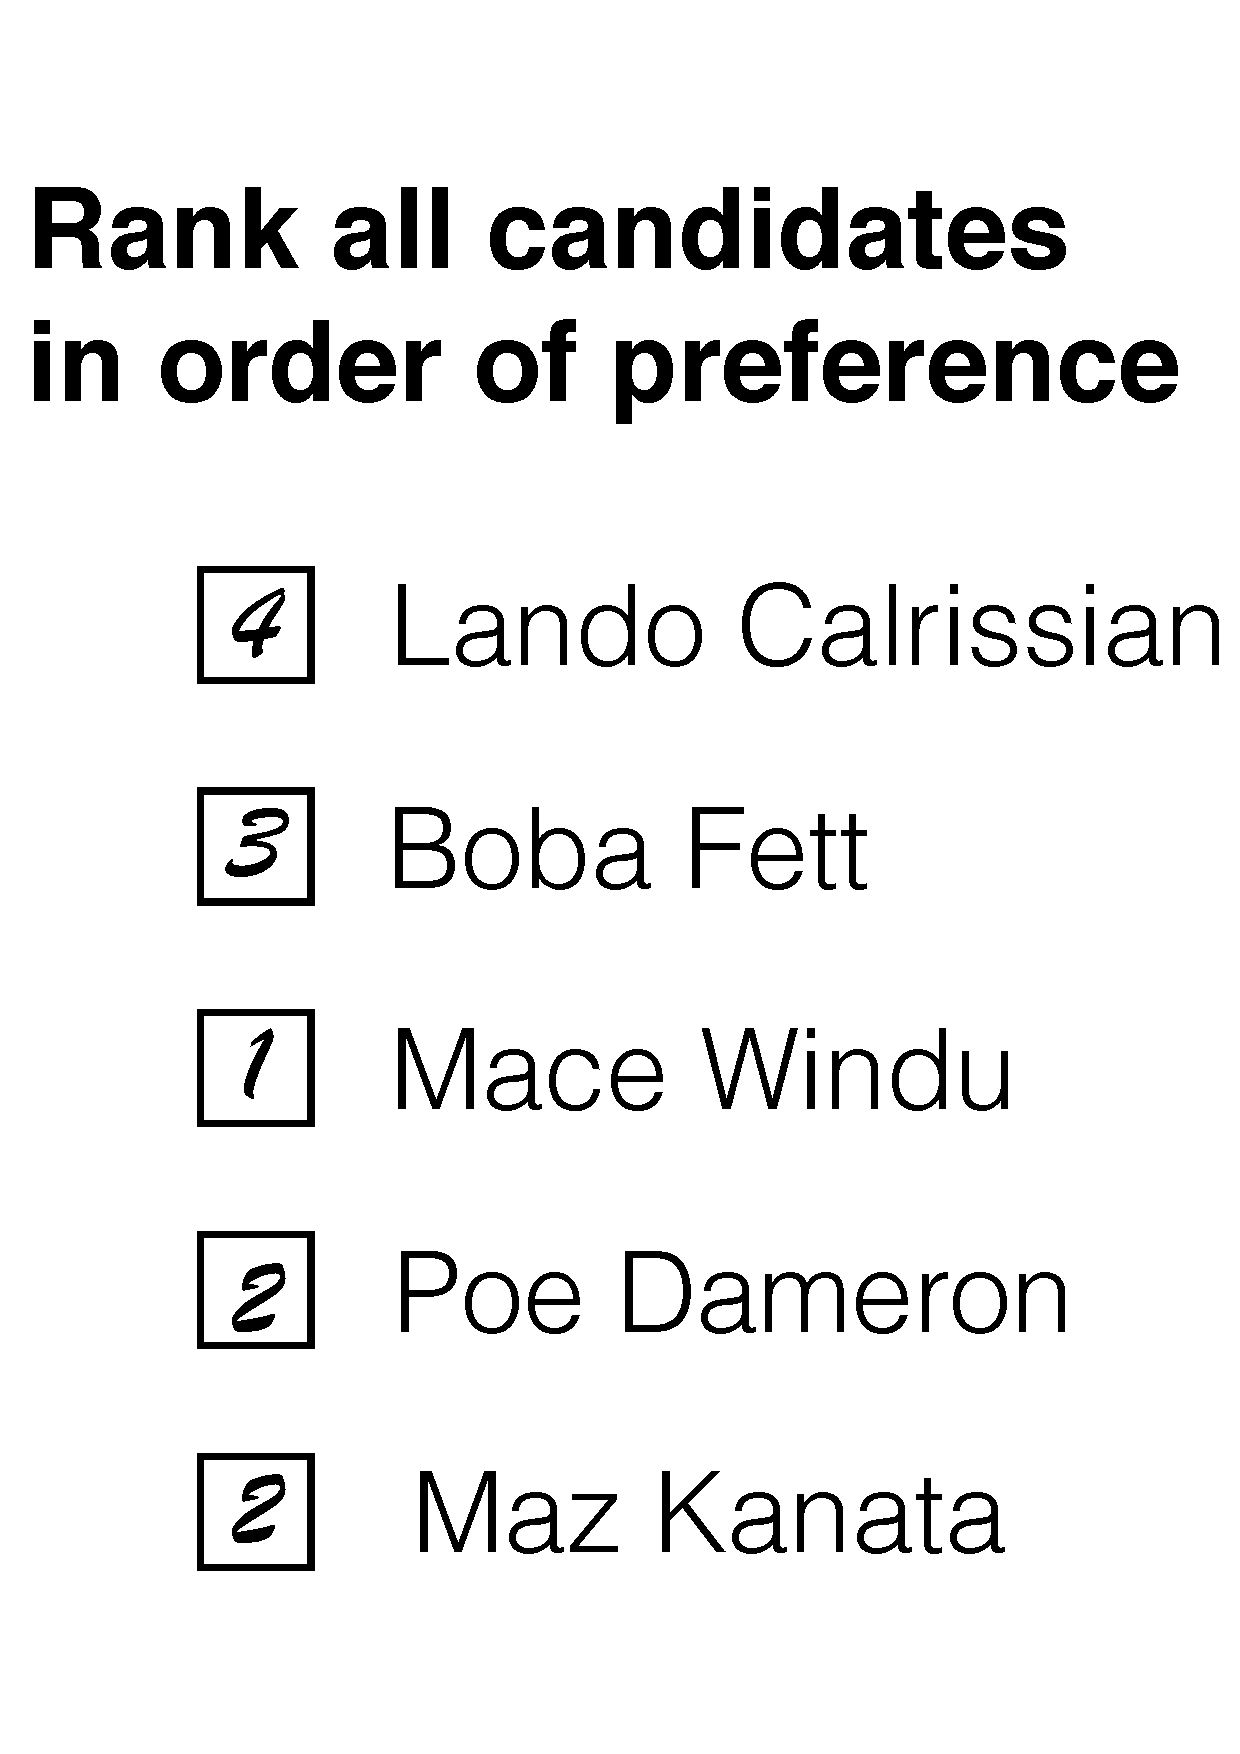
\includegraphics[width=0.37\textwidth]{bal-cropped.pdf}}
    \vspace*{-8ex}
    %\raisebox{0pt}[\dimexpr\height-8.5\baselineskip\relax]{xx}
    %\includegraphics[width=4cm]{ballot.png}
  \end{center}
\end{wrapfigure}
In practice, ballots are
implemented by asking voters to put numerical preferences against
the names of candidates as represented by the image on the right.
The most natural representation of a ballot is therefore a function
$b: C \to Nat$ that assigns a natural number (the preference) for
each candidate, and we recover a strict linear preorder $<_b$ on candidates
by setting $c <_b d$ if $b(c) > b(d)$. 

As preferences are usually
numbered beginning with $1$, we interpret a preference of $0$ as the
voter failing to designate a preference for a candidate
as this allows us to also accommodate incomplete ballots.
This is clearly a design decision, and we could have formalised
ballots as functions $b: C \to 1 + Nat$ (with $1$ being the unit
type) but it would add little to our analysis.
%
%
\begin{verbatim}
  Definition ballot := cand -> nat.
\end{verbatim}

\noindent
The count of an individual election is then parameterised by the list
of ballots cast, and is represented as a dependent inductive type.
More precisely, we have a type \texttt{State} that represents either
an
intermediate stages of constructing the margin function or the
determination of the final election result:
\begin{verbatim}

  Inductive State: Type :=
  | partial: (list ballot * list ballot)  -> (cand -> cand -> Z) -> State
  | winners: (cand -> bool) ->  State.

\end{verbatim}

\noindent
The interpretation of this type is that a state either consists of
two lists of ballots and a margin function, representing

\begin{itemize}
  \item the set of ballots counted so far, and the set of invalid
ballots seen so far
  \item the margin function constructed so far
\end{itemize}
or, to signify that winners have been determined, a boolean function
that determines the set of winners.

The type that formalises correct counting of votes according to the
Schulze method is parameterised by the profile of ballots cast (that
we formalise as a list), and depends on the type \texttt{State}. That
is to say, an inhabitant of the type \texttt{Count n}, for
\texttt{n} of type \texttt{State}, represents a correct execution of
the voting protocol up to reaching state \texttt{n}. This
state generally represents intermediate stages of the construction
of the margin function, with the exception of the final step where
the election winners are being determined. The inductive type takes
the following shape:

\begin{verbatim}
  Inductive Count (bs : list ballot) : State -> Type :=
  | ax us m : us = bs -> (forall c d, m c d = 0) -> 
    Count bs (partial (us, []) m)         (* zero margin      *)
  | cvalid u us m nm inbs : Count bs (partial (u :: us, inbs) m) -> 
    (forall c, (u c > 0)%nat) ->          (* u is valid       *)
    (forall c d : cand, 
      ((u c < u d) -> nm c d = m c d + 1) (* c preferred to d *) /\
      ((u c = u d) -> nm c d = m c d)     (* c, d rank equal  *) /\
      ((u c > u d) -> nm c d = m c d - 1))(* d preferred to c *) ->
    Count bs (partial (us, inbs) nm)
  | cinvalid u us m inbs : Count bs (partial (u :: us, inbs) m) -> 
    (exists c, (u c = 0)%nat)             (* u is invalid     *) ->
    Count bs (partial (us, u :: inbs) m)
  | fin m inbs w (d : (forall c, (wins_type m c) + (loses_type m c))):
    Count bs (partial ([], inbs) m)       (* no ballots left  *) ->
    (forall c, w c = true <-> (exists x, d c = inl x)) ->
    (forall c, w c = false <-> (exists x, d c = inr x)) ->
    Count bs (winners w).
 
\end{verbatim}

\noindent
The intuition here is simple: the first constructor, \texttt{ax},
initiates the construction of the margin function, and we ensure
that all ballots are uncounted, no ballot are invalid (yet), and the
margin function is constantly zero. The second constructor,
\texttt{cvalid}, updates the margin function according to a valid
ballot (all candidates have preferences marked against their name),
and removes the ballot from the list of uncounted ballots. The
constructor \texttt{cinvalid} moves an invalid ballot to the list of
invalid ballots, and the last constructor \texttt{fin} applies only
if the margin function is completely constructed (no more uncounted
ballots). In its arguments, \texttt{w: cand -> bool} is the function
that determines election winners, and \texttt{d} is a function that
delivers, for every candidate, type-level evidence of winning or
losing, consistent with \texttt{w}. Given this, we can conclude the
count and declare \texttt{w} to be the set of winners (or more
precisely, those candidates for which \texttt{w} evaluates to
\texttt{true}). 

Together with the equivalence of the propositional notions of
winning or losing a Schulze count with their type-level
counterparts, every inhabitant of the type \texttt{Count b (winners
w)} then represents a correct count of ballots \texttt{b} leading to
the boolean predicate \texttt{w: cand -> bool} that determines the
winners of the election with initial set \texttt{b} of ballots.

The crucial aspect of our formalisation of executions of Schulze
counting is that the transcript of the count is represented by a
type that is \emph{not} a proposition. As a consequence, extraction
delivers a program that produces the (set of) election winner(s),
\emph{together} with the evidence recorded in the type to enable
independent verification.




\subsection{All Schulze Election Have Winners}
\label{sec:all_winners}
The main theorem, the proof of which we describe in this section, is
that all elections according to the Schulze method engender a
boolean-valued function \texttt{w: cand -> bool}
that determines
precisely which candidates are winners of the election, together
with type-level evidence of this.
Note that a Schulze election can have more
than one winner, the simplest (but not the only) example being when
no ballots at all have been cast.
The theorem that we establish (and later extract as a program)
simply states that for every incoming set of ballots, there is a
boolean function that determines the election winners, together with
an inhabitant of the type \texttt{Count} that witnesses the
correctness of the execution of the count. In Coq, we use a
type-level existential quantifier \texttt{existsT} where
\texttt{existsT (x:A), P} stands for $\Sigma_{\mathtt{x:A}}
\texttt{P}$.

\begin{verbatim}
  Theorem schulze_winners: forall (bs : list ballot),
    existsT (f : cand -> bool) (p : Count bs (winners f)), True.
\end{verbatim}


\noindent
The first step in the proof is elementary: We show that for any
given
list of ballots we can reach a state of the count where there are
no more uncounted ballots, i.e. the margin function has been
fully constructed.


\begin{verbatim}

Lemma all_ballots_counted: forall (bs : list ballot), 
        existsT i m, (Count bs (partial ([], i) m)).
        
\end{verbatim}
    

\iffalse
The second step is more involved: given the margin function, we
construct an integer-valued matrix \texttt{M: cand -> cand -> Z}
with the property that \texttt{M c d} is the strength of the
strongest path between \texttt{c} and \texttt{d}. It is intuitively
clear that in this construction, we only need to consider paths
without repeated nodes, i.e. paths that are of length at most $n$,
where $n$ is the number of candidates. Technically, we define an
iterated margin function $M_i: C \times C \to Z$ by putting
$M_0 (c, d) = m(c, d)$ and
\[ M_{i+1}(c, d) = \max \lbrace M_i(c, d), \max \lbrace  \min
\lbrace m(c, e), M_i(e, d) \mid e \in C \rbrace \rbrace \rbrace
\] for $i \geq 0$.
The intuition is that $M_i(c, d)$ is the strength of the strongest
path of length $< i$ that connects $c$ with $d$. The key lemma is
the following:

The following are equivalent for candidates $c$, $d$,
$k \in Nat$ and $s \in Z$:
\begin{enumerate}
\item $M_k(c, d) \geq s$
\item there is $j \leq k$ and a list $(c_1, \dots,
c_j)$ so that the strength of $(c, c_1, \dots, c_j, d)$ is
$\geq s$.
\end{enumerate}

\fi
   
   
The second step relies on the iterated margin function already
discussed in Section \ref{sec:prop-type}. As $M_n(c, d)$ (for $n$ being
the number of candidates) is the strength of the strongest path
between $c$ and $d$, we construct a boolean function
$w$ such that $w(c) = \mathtt{true}$ if and only if $M_n(c, d) \geq
M_n(d, c)$ for all $d \in C$. We then construct the type-level
evidence required in the constructor \texttt{fin} 
using  the function (or proposition)
\texttt{iterated\_marg\_wins\_type} described earlier. 


\section{Scrutiny Sheet and Experimental Result}
\label{sec:scrunity_sheet}
	The crucial aspect of our formalisation is that the vote counting
protocol itself is represented as a dependent inductive type
that represents all (correct) partial executions of
the protocol.  A complete execution is can then be understood as a
state of vote counting where election winners have been determined.
Our main theorem then asserts that an inhabitant of this type
exists, for all possible sets of incoming ballots. 
Crucially, every such inhabitant contains enough information
to (independently) verify the correctness of the election result,
and can be thought of as a \emph{certificate} for the count.

From a computational perspective, we view tallying not merely as a
function that delivers a result, but instead as a function that
delivers a result, \emph{together} with evidence that allows us to
verify correctness. In other words, we augment verified correctness
of an algorithm with the means to verify each particular
\emph{execution}.

Todo : This already introduces software independence. Try 
to refer to that section. Universal verifiability.

From the perspective of electronic voting, this means that
we no longer need to trust the hardware and software
that was employed to obtain the election result, as the generated
certificate can be verified independently. In the literature on
electronic voting, this is known as \emph{verifiability} and has
been recognised as one of the cornerstones for building trust in
election outcomes \citep{Chaum:2004:SBR}, and is the only answer to
key questions such as the possibility of hardware malfunctions, or
indeed running the very software that has been claimed to count
votes correctly.

The certificate that is produced by each run of our extracted Schulze vote
tallying algorithm  consists of two parts. The first part details
the individual steps of constructing the margin function, based on
the set of all ballots cast. The second part presents evidence for
the determination of winners, based on generalised margins. For the
construction of the margin function, every ballot is processed
in turn, with the margin between each pair of votes updated
accordingly.  The heart of our work lies in this second part of the
certificate. To demonstrate that candidate $c$ is an election
winner, we have to demonstrate that the generalised margin between
$c$ and every other candidate $d$ is at least as large than the
generalised margin  between $d$ and $c$. Given that the generalised margin
between two candidates $c$ and $d$ is determined in terms of
paths $c, c_1, \dots, c_n, d$ that join $c$
and $d$, we need to exhibit
\begin{itemize}
\item evidence for the existence of a path $p$ from $c$ to $d$
\item evidence for the fact that \emph{no} path $q$ from $d$ to $c$
is stronger than $p$
\end{itemize}
where the strength of a path $p = (c_0, \dots, c_{n+1})$ is the
minimum $\min \lbrace m(c_i, c_{i+1}) \mid 0 \leq i \leq n \rbrace$
of the margins between adjacent nodes.  While evidently a path
itself is evidence for its existence, the \emph{non-existence} of
paths with certain properties is more difficult to establish. For this,
we uses a coinductive approach. As existence of a path with a given
strength between two candidates can be easily phrased as an
inductive definition, the \emph{complement} of this predicate arises
as a greatest fixpoint, or equivalently as a coinductively defined
predicate (see e.g. \citep{Kozen:2016:PC}). This allows us to witness
the non-existence of paths by exhibiting co-closed sets.
  

Coq's extraction mechanism then allows us to turn this into a
provably correct program. When extracting, all purely propositional
information is erased and given a set of incoming ballots, the ensuing program produces an inhabitant
of the (extracted) type \texttt{Count} that records the construction
of the margin function, together with (type level) evidence of
correctness of the determination of winners. That is, we see the
individual steps of the construction of the margin function (one
step per
ballot) and once all ballots are exhausted, the determination of
winners, together with paths and co-closed sets. The following is
the transcript of a Schulze election where we have added wrappers
to pretty-print the information content. This is the (full) scrutiny
sheet promised in Section \ref{sec:prop-type}.
%
%\newpage
\begin{footnotesize}
\begin{verbatim}
V: [A3 B1 C2 D4,..], I: [], M: [AB:0 AC:0 AD:0 BC:0 BD:0 CD:0]
--------------------------------------------------------------
V: [A1 B0 C4 D3,..], I: [], M: [AB:-1 AC:-1 AD:1 BC:1 BD:1 CD:1]
----------------------------------------------------------------
V: [A3 B1 C2 D4,..], I: [A1 B0 C4 D3], M: [AB:-1 AC:-1 AD:1 BC:1 BD:1 CD:1]
---------------------------------------------------------------------------
                     . . .
----------------------------------------------------------------------
V: [A1 B3 C2 D4], I: [A1 B0 C4 D3], M: [AB:2 AC:2 AD:8 BC:5 BD:8 CD:8]
----------------------------------------------------------------------
V: [], I: [A1 B0 C4 D3], M: [AB:3 AC:3 AD:9 BC:4 BD:9 CD:9]
-----------------------------------------------------------
winning: A
  for B: path A --> B of strenght 3, 4-coclosed set: 
    [(B,A),(C,A),(C,B),(D,A),(D,B),(D,C)]
  for C: path A --> C of strenght 3, 4-coclosed set:
    [(B,A),(C,A),(C,B),(D,A),(D,B),(D,C)]
  for D: path A --> D of strenght 9, 10-coclosed set:
    [(D,A),(D,B),(D,C)]
losing: B
  exists A: path A --> B of strength 3, 3-coclosed set:
    [(A,A),(B,A),(B,B),(C,A),(C,B),(C,C),(D,A),(D,B),(D,C),(D,D)]
losing: C
  exists A: path A --> C of strength 3, 3-coclosed set:
    [(A,A),(B,A),(B,B),(C,A),(C,B),(C,C),(D,A),(D,B),(D,C),(D,D)]
losing: D
  exists A: path A --> D of strength 9, 9-coclosed set:
    [(A,A),(A,B),(A,C),(B,A),(B,B),(B,C),(C,A),(C,B),(C,C),(D,A),(D,B),
     (D,C),(D,D)]  
\end{verbatim}
\end{footnotesize}

\noindent
Here, we assume four candidates, \texttt{A}, \texttt{B}, \texttt{C}
and \texttt{D} and a ballot of the form \texttt{A3  B2  C4  D1}
signifies that \texttt{D} is the most preferred candidate (the first
preference), followed by \texttt{B} (second preference), \texttt{A}
and \texttt{C}. In every line, we only display the first uncounted
ballot (condensing the remainder of the ballots to an ellipsis),
followed by votes that we have deemed to be invalid. We display the
partially constructed margin function on the right. Note that the
margin function satisfies  $m(x, y) = -m(y, x)$ and $m(x, x) = 0$ so
that the margins displayed allow us to reconstruct the entire margin
function. In the construction of the margin function, we begin with
the constant zero function, and going from one line to the next, the
new margin function arises by updating according to the first
ballot. This corresponds to the constructor \texttt{cvalid} and
\texttt{cinvalid} being
applied recursively: we see an invalid ballot being set aside in the
step from the second to the third line, all other ballots are valid.
Once the margin function is fully constructed (there are no
more uncounted ballots), we display the evidence provided in the
constructor \texttt{fin}: we present evidence of winning (losing) for
all winning (losing) candidates. 
%
In order to actually verify the computed result, a third party
observer would have to
\begin{enumerate}
\item Check the correctness of the individual steps of computing the
margin function
\item For winners, verify that the claimed paths exist with the
claimed strength, and check that the claimed sets are indeed
coclosed.
\end{enumerate}

\noindent
Contrary to re-running a different implementation on the same
ballots, our scrutiny sheet provides an \emph{orthogonal}
perspective on the data and how it was used to determine the
election result.

We have evaluated our approach by extracting the entire Coq
development into Haskell, with all types defined by Coq extracted as
is, i.e. in particular using Coq's unary representation of natural
numbers. The results are displayed in Figure \ref{fig:straight}
using a logarithmic scale. 


%\begin{figure}
%\centering
%\begin{minipage}{.5\textwidth}
%  \centering
%  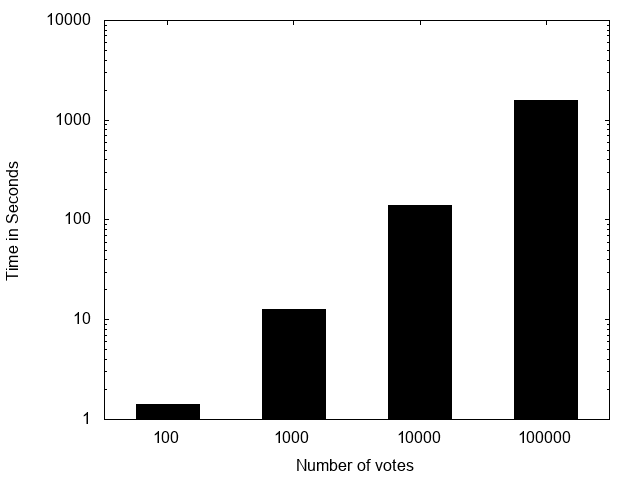
\includegraphics[width=1.0\linewidth]{1.png}
%  \caption{Direct Extraction}
%  \label{fig:straight}
%\end{minipage}
%\begin{minipage}{.5\textwidth}
%  \centering
%  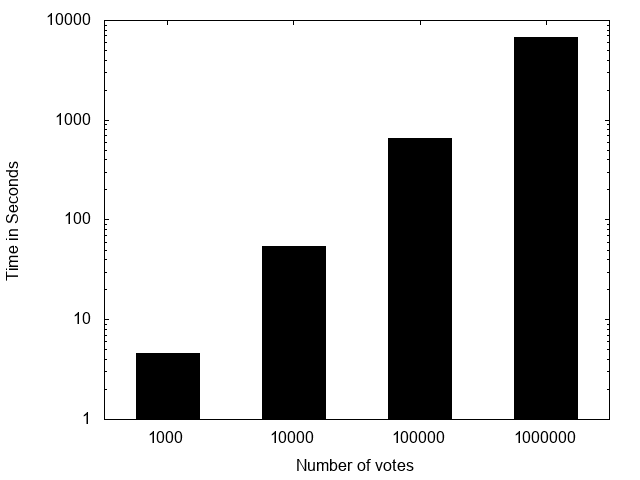
\includegraphics[width=1.0\linewidth]{2.png}
% \caption{Extraction using Haskell Integers}
% \label{fig:native}
%\end{minipage}
%\caption{Experimental Results}
%\label{fig:test}
%\end{figure}


\begin{figure}
\centering     %%% not \center
\subfigure[Direct Extraction]{\label{fig:straight}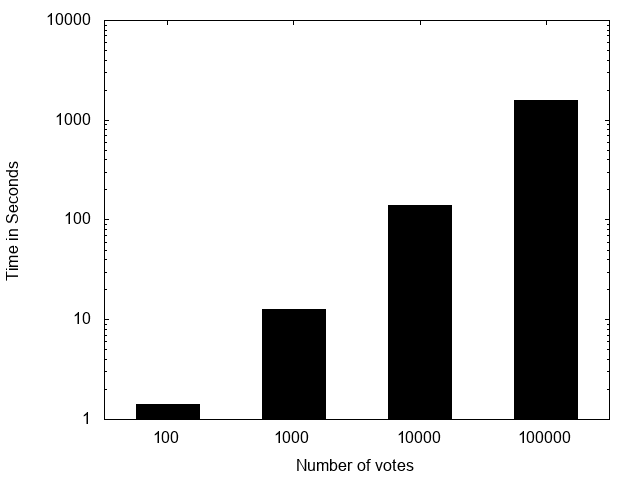
\includegraphics[width=60mm]{1.png}}
\subfigure[Extraction using Haskell Integers]{\label{fig:native}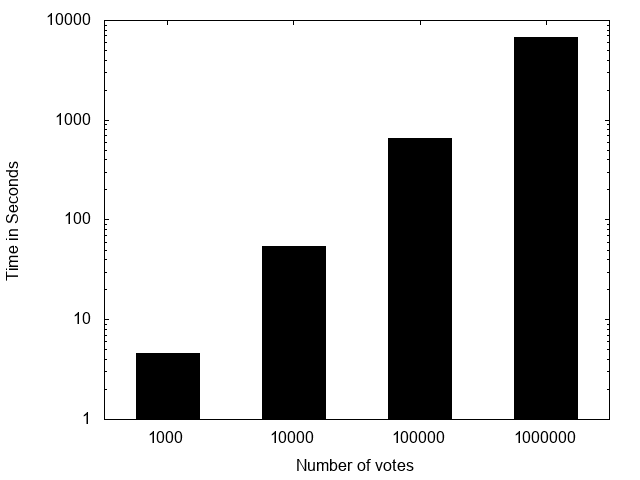
\includegraphics[width=60mm]{2.png}}
\caption{Experimental Results}
\label{fig:test}
\end{figure}

%
%\begin{figure}
%\centering
%\begin{subfigure}
%  \centering
%  {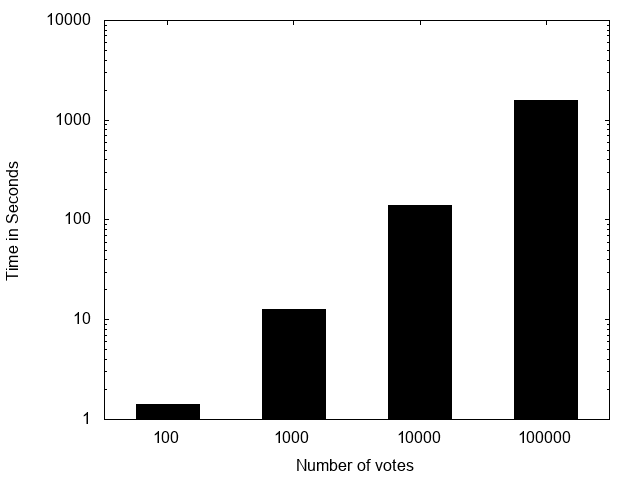
\includegraphics[width=.95\textwidth]{1.png}}
%  \caption{Direct Extraction}
%  \label{fig:straight}
%\end{subfigure}%
%\end{figure}
%\begin{figure}
%\begin{subfigure}
%  \centering
%  {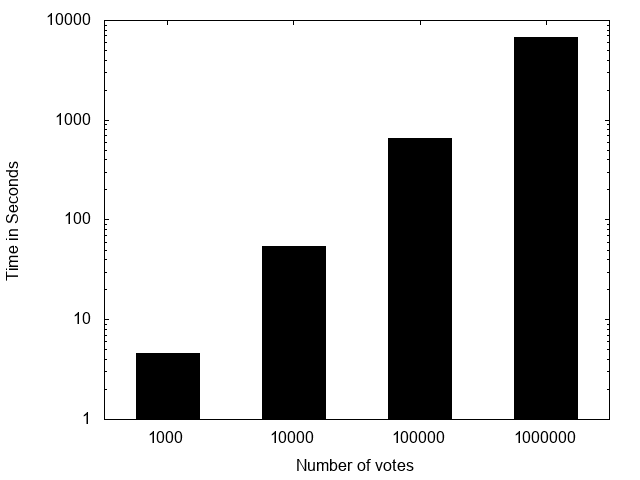
\includegraphics[width=.95\textwidth]{2.png}}
%  \caption{Extraction using Haskell Integers}
%  \label{fig:native}
%\end{subfigure}
%\caption{Experimental Results}
%\label{fig:test}
%\end{figure}
  
 \section{Scaling it count millions of Ballots}
 \label{sec:count_million}
 We investigated the extracted Haskell code  from Coq code.
The most performance critical aspect of our code was the computation of  margin
function. Recall that the margin function is of type
\texttt{cand -> cand -> Z}
and that it depends on the \emph{entire} set of ballots. Internally, it is
represented by a closure \citep{Landin:1964:MEE} so that margins are
re-computed with every call. The single largest efficiency
improvement in our code was achieved by memoization, i.e.
representing the margin function (in Coq) via list lookup. With
this (and several smaller) optimisation, we can count millions of
votes using verified code. Below, we include our timing graphs,
based on randomly generated ballots while keeping number of candidates
constant i.e. 4. 


\begin{figure}
\centering     %%% not \center
\subfigure[Computation of Winners]{\label{fig:straight}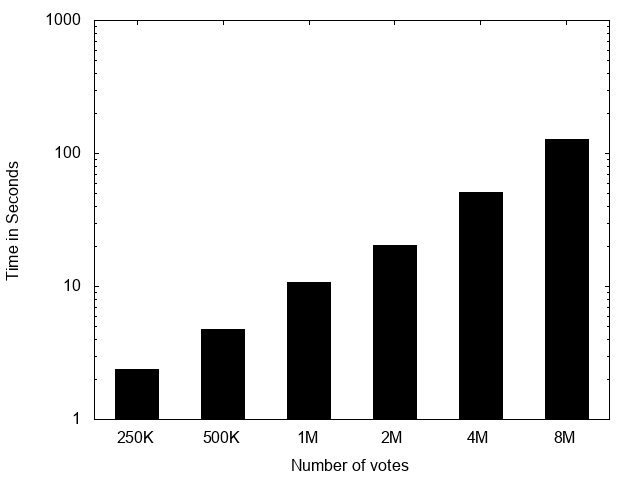
\includegraphics[width=60mm]{without-cert.png}}
\subfigure[Computation of Winners and Certificate]{\label{fig:native}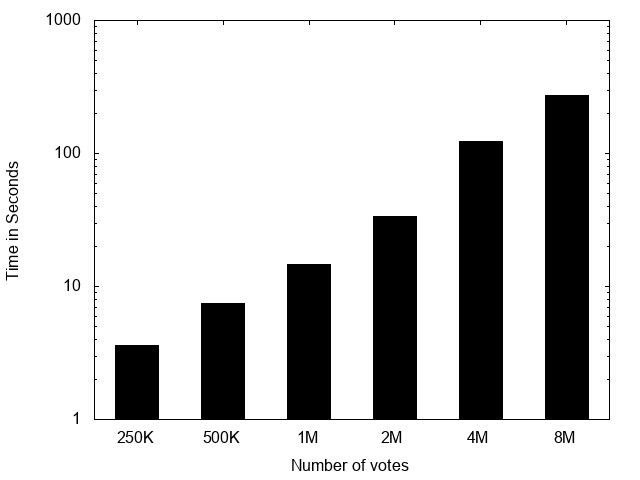
\includegraphics[width=60mm]{with-cert.png}}
\caption{Experimental Results}
\label{fig:test}
\end{figure}


%\begin{figure}
%\centering
%\begin{subfigure}{.5\textwidth}
%  \centering
%  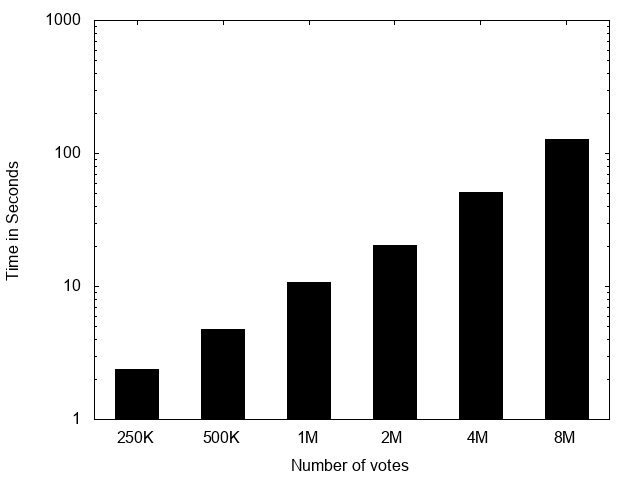
\includegraphics[width=.95\textwidth]{without-cert.png}
%  \caption{Computation of Winners}
%  \label{fig:straight}
%\end{subfigure}%
%\begin{subfigure}{.5\textwidth}
%  \centering
%  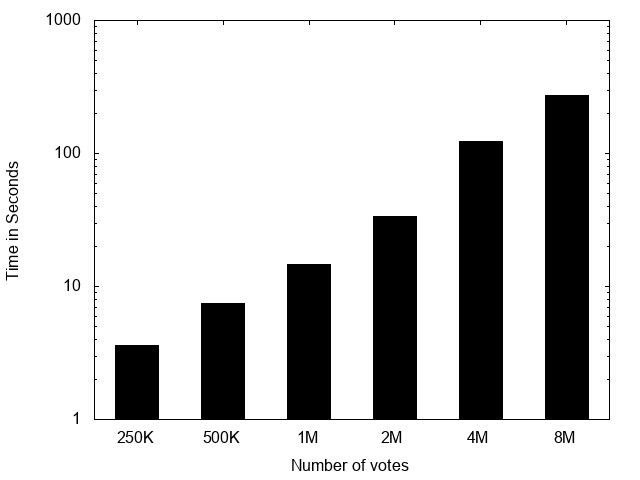
\includegraphics[width=.95\textwidth]{with-cert.png}
%  \caption{Computation of Winners and Certificate}
%  \label{fig:native}
%\end{subfigure}
%\caption{Experimental Results}
%\end{figure}

\noindent
On the left, we report timings (in seconds) for the computation of
winners, whereas on the right, we include the time to additionally
compute a universally verifiable certificate that attests  to the
correctness of the count. This is consistent with complexity of Schulze 
counting i.e. linear in no of ballots and cubic in candidates. 
The experiments were carried out on system 
equipped with intel core i7 processor and 16 GB of ram. We notice that the
computation of the certiciate adds comparatively little in
computational cost. 

Our implementation requires that we store \emph{all}
ballots in main memory as we need to parse the entire list of
ballots before making it available to our verified implementation so
that the total number of ballots we can count is limited by main
memory in practise. We can count real-world size elections (8
million ballot papers) on a standard, commodity desktop computer with
16 GB of main memory. 

  
\section{Discussion} \label{sec:discussion}

In this chapter,  we emphasize on correctness, 
and we take the approach that 
computation of winners in
electronic voting (and in situations where correctness is key in
general) should not only produce an end result, but an end result,
\emph{together} with a verifiable justification of the correctness
of the computed result. In this paper, we have exemplified this
approach by providing a provably correct, and evidence-producing
implementation of vote counting according to the Schulze method. 

While the Schulze method is not difficult to implement, and indeed
there are many freely available implementations, comparing the
results between different implementations can give some level of
assurance for correctness only in case the results agree.  If there
is a discrepancy, a certificate for the correctness of the count
allows to adjudicate between different implementations, as the
certificate can be checked with relatively little computational
effort. 

From the perspective of computational complexity, checking a
transcript for correctness is of the same complexity as computing
the set of winners, as our certificates are cubic in size, so that
certificate checking is not less complex than the actual
computation. 

However, publishing an independently verifiable certificate that
attests the individual steps of the computation helps to increase
\emph{trust} in the computed election outcome. Typically, the use of technology in
elections increases the amount of trust that we need to place both
in technological artefacts, and in people. It raises questions that
range from fundamental aspects, such as proper testing and/or
verification of the software, to very practical questions, e.g.
whether the correct version of the software has been run.  On the
contrast, publishing a certificate of the count dramatically reduces
the amount of trust that we need to place into both people and
technology: the ability to publish a verifiable justification of the
correctness of the count allows a large number of individuals to
scrutinise the count. While only moderate programming skills are
required to check the validity of a certificate (the transcript of
the count), even individuals without any programming background can
at least spot-check the transcript: for the construction of the
margin function, everything that is needed is to show that the
respective margins change according to the counted ballot. For the
correctness of determination of winners, it is easy to verify
existence of paths of a given strength, and also whether certain
sets are co-closed -- even by hand! This dramatically increases the
class of people that can scrutinise the correctness of the count,
and so helps to establish a trust basis that is much wider as no
trust in election officials and software artefacts is required.

Technically, we do not \emph{implement} an algorithm that counts
votes according to the Schulze method. Instead, we give a
specification of the Schulze winning conditions 
(\texttt{wins\_prop} in  Section \ref{sec:spec}) in terms of an
already computed margin function that
(we hope) can immediately be seen to be correct, and then show that those
winning conditions are equivalent to the existence of inhabitants of
types that carry verifiable evidence (\texttt{wins\_type}).  We then
join the (type level) winning conditions with an inductive type that
details the construction of the margin function in an inductive
type. Via propositions-as-types, a provably correct vote counting
function is then equivalent the proposition that there exists an
inhabitant of \texttt{Count} for every set of ballots.  Coq's
extraction mechanism then allows us to extract a Haskell program
that produces election winners, together with verifiable
certificates. 

%\section{Summary}

%In this formalization, we have presented a formalisation of 
%the Schulze method for
%counting preferential ballots. Our formalisation focuses on the
%correct execution of the method. 
%In our formalisation of vote counting, there is a one-to-one
%correspondence between correct executions of the protocol, and
%inhabitants of a (dependent) inductive type. In our Coq development,
%we have used the propositions-as-types approach, and have
%constructed an existence proof, from which we have generated Haskell
%code. An alternative approach would be to implement a function that
%directly constructs inhabitants, and obtain a detailed performance
%comparison between both approaches. While we anticipate that a
%direct implementation brings performance benefits, our experimental
%evaluation shows that even with very little optimisation (Section
%\ref{sec:eval}), extracting
%vote counting program from an existence proof allows us to count a
%relatively large number of ballots already.

Our formalization achieves \textit{Correctness}, \textit{Practicality}, and 
(tallied-as-cast) \textit{Verifiability}. The major wrinkle in this formalization is \textit{Privacy}.  
Our ballots are in plaintext and could easily be identified
if the number of candidates participating in election in 
are large (Italian attack) \citep{Otten}.
\noindent
In nutshell, the pros and cons of this formalization:

\begin{itemize}
\item Pros 
\begin{itemize}
\item Correctness: The implementation is formalized in Coq with emphasis on generating 
         evidence to convince everyone about the outcome of election.
\item Practicality: The extracted code can count millions of ballots. Therefore, we can use it 
          in any real life election.
\item Verifiability: The outcome of any election can be verified by any third party because 
          of the generated certificates. Certificates generated for plaintext ballot 
		  during the election 
          are very simple.  It requires basic math literacy to audit the certificate which would 
          lead to increase in number of scrutineers. 

\end{itemize}
\item Cons
\begin{itemize}
\item Privacy : There is no privacy, and possibly susceptible to coercion, because the ballots involved 
         are simply plaintext. 
\end{itemize}
\end{itemize}

 In the next chapter, we will try to solve privacy problem, possibly coercion, using encryption, and to keep 
 it verifiable, we will use zero-knowledge-proof. However, solution for privacy comes with other cost, e.g. 
 loss in pool of scrutineers because auditing a certificate generated by counting encrypted ballot 
 would requires intricate knowledge of cryptography.  
 
We remark that extracting Coq developments into a
programming language itself is a non-verified process which could
still introduce errors in our code. The most promising way to
alleviate this is to independently implement (and verify) a
certificate verifier, possibly in a language such as CakeML
\citep{Kumar:2014:CVI} that is guaranteed to
be correct to the machine level. 

\chapter{Homomorphic Schulze Algorithm : Axiomatic Approach}
\label{cha:homormorphic_schulze}

\epigraph{Be melting snow. Wash yourself of yourself.} 
{\textit{Rumi}} 

\section{Introduction}
As we stated in the  summary of last chapter that plaintext could lead to 
privacy problems, e.g. ballot identification (Italian attack) \cite{Otten}. 
In this chapter, we achieve privacy by using encryption, (tallied-as-cast) 
verifiability by using zero-knowledge proof, and correctness of implementation 
by proving the correctness properties inside the Coq theorem prover. 
One important point to note that we do not formalize any cryptographic primitive inside the Coq, but 
take an axiomatic approach, i.e. we assume the existence of cryptographic 
primitives and postulate their correctness property (axiomatisation of 
cryptographic primitives).  The reason for axiomatic approach is
because our goal is to not formalise the cryptographic primitives, but use these primitives
to conduct an election which has all three ingredients, privacy, verifiability, 
and correctness. We then obtain, via program extraction, a
provably correct implementation of vote counting, that we turn
into executable code by providing implementations of the cryptographic primitives
based on a standard cryptographic library (Unicrypt). 
We conclude by presenting
experimental results, and discuss the trust base, security, and
privacy as well as the applicability of our work to real-world
scenarios. 




\textbf{Chapter Outline:} In Section \ref{sec:verifiable_homomorphic}, 
we discuss the technique to achieve verifiable homomorphic tally. In order to do so, 
we discuss why do we need our ballot to have a matrix representation 
and not a ranking function. Moreover, we discuss the concept 
of validity of a ballot, which comes naturally with matrix representation, 
steps of homomorphic counting, and cryptographic primitives needed 
to achieve all the required functionality. Section \ref{sec:realisation} 
takes a step forward and makes every concept from the previous section
concrete using the Coq theorem prover. One important point 
in this section is our inductive data type \textit{ECount}
augmented with verification data in form of zero-knowledge proof 
for various claims made during the counting 
($ECount$ is conceptually similar to the $Count$ (Section \ref{sec:inductive_type}), but 
in terms of data, $ECount$ has state data related to counting and verification data
in form of zero-knowledge proof, while $Count$ 
has just state data).  In Section \ref{sec:correct}, we present
our main theorem which states that for any set of given encrypted ballots, 
a winner can always be found. Apart from the main theorem, this section 
also incorporates the proof of correctness by stating 
the winners produced by encrypted ballots are same as 
plaintext ballots (Section \ref{sec:all_winners}) if 
 the encrypted ballots decrypt to the plaintext ballot. 
 Section \ref{sec:extract} focuses on extraction, instantiating 
 the cryptographic primitives with UniCrypt library, and 
 experimental results. Finally, Section \ref{sec:summary_homomorphic} 
 highlights our assumptions, scalability issues, the 
 goals we achieved and the goals we missed. 


 


Secure elections are a balancing act between integrity and privacy:
achieving either is trivial but their combination is notoriously hard.
One of the key challenges faced by both paper based and electronic
elections is that results must be substantiated with
verifiable evidence of their correctness while retaining the secrecy
of the individual ballot \citep{Bernhard:2017:PES}. 
The combination of privacy and integrity can be realised using cryptographic techniques, where
encrypted ballots (that the voters themselves cannot decrypt) are
published on a bulletin board, and the votes are then processed, and
the correctness of the final tally is substantiated, using
homomorphic encryption \citep{Hirt:2000:ERF} and verifiable shuffling
\citep{Bayer:2012:EZK}. (Separate techniques exist to prevent ballot
box stuffing and to guarantee cast-as-intended.)
Integrity can then be guaranteed by means of zero-knowledge proofs
(ZKP),
first studied by Goldwasser, Micali, and Rackoff~\citep{Goldwasser:1985:STOC}.
Informally, a ZKP is a probabilistic and interactive proof where one
entity interacts with another such that the interaction provides
no information other than that the statement being proved is true with
overwhelming probability. 
Later results~\citep{Ben-Or:1988:CRYPTO,Goldreich:1991:ACM}
showed that 
all problems for which solutions can be efficiently verified have zero-knowledge
proof (in practice,  Sigma protocol \citep{10.1007/3-540-48658-5_19} is used 
to prove the knowledge of a (private) witness $w$ for a public input $x$, 
and it is required to be zero-knowledge against the honest verifier).

  
 \section{Verifiable Homomorphic Tallying}
\label{sec:verifiable_homomorphic}
The realisation of verifiable homomorphic tallying that we are about to
describe follows the same two phases as the Schulze algorithm (described in section \ref{sec:schulze_algorithm}): 
we first homomorphically compute the margin matrix from encrypted ballots, and then compute
winners on the basis of the (decrypted) margin. Moreover, the computation also
produces a verifiable certificate that leaks no information about
choices in individual ballots other than the (final) margin matrix, which in
turn leaks no information about individual ballots if the number of
voters is large enough.  


\subsection{Format of Ballots} 
Recall that in preferential voting
schemes, ballots are rank-ordered lists of candidates. For the
Schulze Method, we require that all candidates are ranked, and two
candidates may be given the same rank. That is, a ballot is most
naturally represented as a function, $C \to \mathbb{N}$, that assigns a
numerical rank to each candidate, and the computation of the margin
amounts to computing the sum
\[ m(x, y) = \sum_{b \in B} \begin{cases} +1 & b(x) < b(y) \\ 0 &
b(x) = b(y) \\ -1 & b(x) > b(y) \end{cases} \]
where $B$ is the multi-set of ballots, and each $b \in B$ is a
ranking function $b: C \to  \mathbb{N}$ over a (finite) set $C$ of
candidates. 

Ideally, we could have copied the same ballot structure in a homomorphic Schulze method, 
but encrypting the choices, i.e. the ballot would have been represented as a function $C \to CT$
where $CT$ (ciphertext) is the encrypted representation of a choice (natural number).
However, we note that this representation of ballots is not well suited for
homomorphic computation of the margin matrix as practically feasible
homomorphic encryption schemes do not support comparison operators
and case distinctions as used in the formula above (to the best of our knowledge).

We instead represent ballots as candidate indexed matrices (represented as function from a pair of candidates to a natural number), 
$C \times C \to \mathbb{N}$,
$bm$ where $bm(x, y) = +1$ if $x$ is preferred
over $y$, $bm(x, y) = -1$ if $y$ is preferred over $x$ and $bm(x, y) =
0$ if $x$ and $y$ are equally preferred. The downside of this representation 
is that it takes $O(n^2)$ space to represent a ballot where $n$ is the number 
of candidate participating in election. 

While the advantage of the first representation, $b: C \to \mathbb{N}$,  is that each ranking
function is necessarily a valid ranking and is linear space ($O(n))$) in the number 
of candidates, $n$, the advantage of the matrix 
representation, $C \times C \to \mathbb{N}$,  is that the computation of
the margin matrix is simple, that is
\[ m(x, y) = \sum_{bm \in B} bm(x, y) \]
where $bm$ is plaintext ballot in matrix form,  and $B$ is the multi-set of ballots (in matrix form). 
The major benefit of this
matrix representation is that it can  be transferred to the encrypted setting in a straight
forward way by encrypting all the entries in $bm$.  We take the advantage of 
matrix representation and represent our encrypted ballot as a matrix of ciphertext, $C \times C \to CT$ (CT stands for ciphertext). 
Following this representation of encrypted ballot,  the encrypted margin can be computed as:
\begin{equation}\label{eqn:enc-mm}
encm(x, y) = \bigoplus_{encb \in EncB} encb(x, y) 
\end{equation}
where $\oplus$ denotes homomorphic addition, $encb$ is an encrypted
ballot in matrix form and $EncB$ is the multi-set of
encrypted ballots. 

 In an ideal world where every voter is honest, 
every entry in $encb$ is either the encryption of -1, 0, or 1. 
Moreover, if we interpret $encb$ as a adjacency matrix of a graph representation, 
$encb$ should be acyclic (lets call it valid or desirable  ballot).  
In addition,  we definitely do not want to be 
in a situation where a voter prefers $A$ over $B$,  $B$ over $C$, 
and finally $C$ over $A$, for some candidates $A$, $B$, and $C$.  
How would we interpret a ballot having cycles? One possible interpretation 
is ranking all the candidates equal appearing a cycle, but clearly it is not a
reasonable interpretation, therefore we 
decided to not include it in final tally (lets call it invalid or undesirable ballot). 
Now during the course of counting encrypted ballots, we need to 
distinguish between a  desirable 
ballot, i.e.  valid ballot, and an undesirable ballot, i.e. invalid ballot.  
To make this distinction,  we verify that 
an encrypted (matrix) ballot $eballot : C \times C \to CT$ is valid only if:
\begin{itemize}
\item  the decryption of $eballot(x, y)$ is indeed one of $1, 0$ or $-1$, where $x$ and $y$ ranges over the list of all candidates
\item  $eballot$ is acyclic (the idea here is that if $eballot$ is acyclic,  then for its decryption, $pballot: C \times C \to \mathbb{Z}$, 
	we can find a ranking function from candidates to natural number, $C \to \mathbb{N}$,  i.e. we can rank all the candidates in a
	linear order (explained in section \ref{sec:valid-pb})).
\end{itemize}

\noindent
More importantly,  to achieve verifiability, we not only need \emph{verify}
that a ballot is valid, we also need to \emph{evidence} its validity
(or otherwise) in the scrutiny sheet.   However,  the issue with the above 
definition,  verification of the validity of an encrypted ballot, is that if we decrypt 
the $eballot$ to the ballot $pballot$ and publish $pballot$  in the scrutiny sheet 
to evidence the validity $eballot$,   
we would reveal the (secret) preference of the voter,  who cast this ballot. 
Therefore, we cannot decrypt the $eballot$, and we need a better way to evidence 
the validity of an encrypted ballot. 


\subsection{Validity of Ballots}
\label{sec:valid-pb}
A plaintext ballot $ptballot : C \times C \to \mathbb{Z}$ 
is \emph{valid} if it is induced by a ranking function, i.e.
there exists a function $f: C \to \mathbb{N}$ such that $ptballot(x, y) = 1$ if
$f(x) < f(y)$, $ptballot(x, y) = 0$ if $f(x) = f(y)$ and $ptballot(x, y) = -1$ if
$f(x) > f(y)$.  In symbols:

\[ ptballot(x, y) =  \exists f : C \to \mathbb{N}  \begin{cases} +1 & f(x) < f(y) \\ 0 &
f(x) = f(y) \\ -1 & f(x) > f(y) \end{cases} \]



\noindent
For a plaintext ballot, it is easy to decide if is valid 
or not valid.  One crucial observation is that if $pballot$ is valid, 
it also valid after permuting its each row and column with the 
same permutation, i.e.  $ptballot$ is valid if and only if $ptballot'$ is 
valid, where
\[ ptballot'(x,y) = ptballot(\pi(x), \pi(y)) \]
and $\pi: C \to C$ is a permutation of candidates.
In fact, if $f : C \to \mathbb{N}$ is a ranking function for $ptballot$, 
$f \circ \pi$ is a ranking function for $ptballot'$.   Also, notice that
if $ptballot$ is the decryption of  $ctballot : C \times C \to CT$
and $ptballot'$ is the decryption of $ctballot' : C \times C \to CT$,  
the following holds:
\[ ctballot'(x,y) = ctballot(\pi(x), \pi(y)) \]


Using these 
ideas, we can evidence the validity of the encrypted ballot,  $ctballot : C \times C \to CT$. 
The ballot $ctballot$ is valid if and only if its decryption  i.e. the plaintext ballot 
$ptballot (x, y) = decb(ctballot (x, y)$ is valid, where $decb : C \times C \to \mathbb{Z}$ 
denotes decryption function, and $x$ and $y$ ranges over the list of candidates. 
However,  as we stated previously, we cannot publish the $ptballot$ as an evidence of validity of 
the $ctballot$ in the scrutiny sheet because then it will leak the 
voter's preference. Thus we generate a secret permutation, $\pi$,  and  subsequently, 
we publish $ctballot'$,  row and column permuted ballot 
of $ctballot$ by the secret permutation $\pi$,  and its decryption $ptballot'$, 
row and column permutation of $ptballot$ by the same secrete permutation $\pi$. 
Moreover,  we augment the scrutiny sheet with the zero-knowledge proofs about various claim, 
e.g. we have decrypted the $ctballot'$ honestly and $ptballot'$ is indeed an honest 
decryption,  the commitment of the secret permutation $\pi$,  etc.  
In a nutshell, we can evidence the validity
of a ciphertext ballot $ctballot$ by
\begin{itemize}
  \item generating a secret permutation, $\pi$ and evidence that it is a valid permutation.
  \item publishing the shuffled version $ctballot'$ of $ctballot$, that is
  shuffled by the secret permutation $\pi$, together with
  evidence that $ctballot'$ is indeed a shuffle of $ctballot$.
  \item publishing the decryption $ptballot'$ of $ctballot'$ together with
  evidence that $ptballot'$ is indeed the decryption of $ctballot'$.
  \item evidencing if $ptballot'$ is valid (or otherwise) by showing the 
  existence of ranking function $f : C \to \mathbb{N}$ (or otherwise).
\end{itemize}

\noindent
We use zero-knowledge proofs (ZKP) in the style of \citep{DBLP:conf/africacrypt/TereliusW10}
to evidence the correctness of the shuffle, and zero-knowledge
proofs of honest decryption \citep{DBLP:conf/crypto/ChaumP92} to evidence
correctness of decryption. This achieves ballot secrecy as
the (secret) permutation is never revealed.


In summary, the evidence of correct (homomorphic) counting starts
with an encryption of the zero margin $encm : C \times C \to CT$ (every entry in 
the $encm$ is an encrypted value of 0), and for each
ciphertext ballot $ctballot : C \times C \to CT $ contains
\begin{enumerate}
\item generation of secret permutation $\pi$  together with a commitment proof and zero-knowledge proof that is a valid permutation
\item \label{it:shuff} $ctballot'$, a shuffle of $ctballot$ by $\pi$ together with a zero-knowledge proof that $ctballot'$ is a shuffle of $ctballot$
\item $ptballot'$, decryption of $ctballot'$, together with a zero-knowledge proof that  $ptballot'$ is  honest decryption of $ctballot'$
\item \label{it:upd-marg}  if $ptballot'$ is valid,  we homorphically  update the margin matrix $encm$,  i.e.   \[ encm(x, y) = encm(x, y) \bigoplus  ctballot(x, y) \]
\item  if the decrypted ballot $ptballot'$ is invalid,  the margin matrix $encm$ remains unchanged
\newcounter{mycnt}
\setcounter{mycnt}{\value{enumi}}
\end{enumerate}
Once all ballots have been processed in this way, the certificate
determines winners and contains
winners by exhibiting
\begin{enumerate}
\setcounter{enumi}{4}
\item \label{it:pub-dm} the final tally $encm$, together with its decryption  
  and a zero-knowledge proof of honest decryption     
\item publishes the winner(s), together with evidence to substantiate the claim (existence of strongest path from the winner to the loser 
and absence of such path from the loser to the winner,  section \ref{sec:evidence}).
\end{enumerate}

\subsection{Cryptographic primitives}
We require an additively homomorphic cryptosystem to
compute the (encrypted) margin matrix according to Equation
\ref{eqn:enc-mm} (this implements Item \ref{it:upd-marg} above). All
other primitives fall into one of three categories.
\emph{Verification primitives} are used to syntactically define
the type of valid certificates. For example, when publishing the
decrypted margin matrix in Item \ref{it:pub-dm} above, we require
that the zero-knowledge proof in fact evidences correct decryption.
To
guarantee this, we need a verification primitive that -- given
ciphertext, plaintext and zero-knowledge proof -- verifies whether the supplied proof
indeed evidences that the given ciphertext corresponds to the given
plaintext. In particular, verification primitives are always boolean
valued functions. While verification primitives \emph{define} valid
certificates, \emph{generation primitives} are used to
\emph{produce} valid certificates. In the example above, we need a
decryption primitive (to decrypt the homomorphically computed
margin) and a primitive to generate a zero-knowledge proof (that
witnesses correct decryption). Clearly verification and generation
primitives have a close correlation, and we need to require, for
example, that zero-knowledge proofs obtained via a generation
primitive has to pass muster using the corresponding verification
primitive. 

The three primitives described above (decryption, generation of a
zero-knowledge proof, and verification of this proof) already allow
us  to implement the entire protocol with exception of ballot
shuffling (Item \ref{it:shuff} above).  Here, the situation is more
complex. While existing mixing schemes (e.g. \citep{Bayer:2012:EZK}) permute 
an array of ciphertexts and produce a zero knolwedge proof that
evidences the correctness of the shuffle, our requirement dictates
that every row and colum of the (matrix) ballot is
shuffled with the \emph{same} (secret) permutation.  In other words,
we need to retain the identity of the permutation to guarantee that
each row and column of a ballot have been shuffled by the same
permutation.
We achieve this by
committing to a permutation using Pedersen's commitment scheme
\citep{Pederson}.
In a nutshell, the Pedersen commitment scheme has the following properties. 
\begin{itemize}
\item Hiding: the commitment reveals no information about the
permutation
\item Binding: no party can open the commitment in more  
	 	than one way, i.e. the commitment is to one permutation only. 
\end{itemize}

\noindent
A combination of Pedersen's commitment scheme 
with a zero-knowledge proof leads to a similar two step protocol, also known 
as commitment-consistent proof of shuffle \citep{Wikstrom:2009:CPS}.

\begin{itemize}
\item Commit to a secret permutation and publish the commitment (hiding).
\item Use a zero-knowledge proof to show that shuffling has used 
      the same permutation which we committed to in previous step (binding).
\end{itemize}  

\noindent
This allows us to witness the validity (or otherwise) of a ballot by generating a 
permutation $\pi$ which is used to shuffle every row and column of the ballot.
We hide $\pi$ by committing it using Pedersen's 
commitment scheme 
and record the commitment $c_{\pi}$ in the certificate. However, for the binding step, rather 
than opening $\pi$ we generate a zero-knowledge proof, $zkp_{\pi}$, 
using $\pi$ and $c_{\pi}$, which can 
be  used to prove that $c_{\pi}$ is indeed the commitment to some permutation
used in the (commitment consistent) shuffling 
 without being opened \citep{Wikstrom:2009:CPS}. We can now use the
 permutation that we have committed to for 
shuffling each row and column of a ballot, and evidence the
correctness of the shuffle via a zero-knowledge proof.
%
To evidence validity (or otherwise) of a (single) ballot, we
therefore:
\begin{enumerate}
  \item generate a (secret) permutation and publish a commitment to this
  permutation, together with a zero-knowledge proof that evidences commitment
  to a permutation
  \item for each row of the ballot, publish a shuffle of the row with
  the permutation committed to, together with a zero-knowledge proof
  that witnesses shuffle correctness
  \item for each column of the row shuffled ballot, publish a
  shuffle of the column, also together with a zero-knowledge proof of
  correctness 
  \item publish the decryption the ballot shuffled in this way, together with a
  zero-knowledge proof that witnesses honest decryption
  \item decide the validity of the ballot based on the decrypted
  shuffle.
\end{enumerate}

\noindent
The cryptographic primitives needed to implement this again fall
into the same classes. To define validity of certificates, we need
verification primitives
\begin{itemize}
  \item to decide whether a zero-knowledge proof evidences that a
  given commitment indeed commits to a permutation 
  \item to decide whether a zero-knowledge proof evidences the
  correctness of a shuffle relative to a given permutation
  commitment.
\end{itemize}

\noindent
Dual to the above, to generate (valid) certificates, we need the
ability to
\begin{itemize}
  \item generate permutation commitments and accompanying zero
  knowledge proofs that evidence commitment to this permutation
  \item generate shuffles relative to a commitment, and zero
  knowledge proofs that evidence the correctness of shuffles.
\end{itemize}

\noindent
Again, both need to be coherent in the sense that the zero-knowledge
proofs produced by the generation primitives need to pass
validation. In summary, we require an additively homomorphic
cryptosystem that implements the following:

\begin{description}
\item[Decryption Primitives.]
  decryption of a ciphertext, creation and verification of
 honest decryption zero-knowledge proofs. 

\item[Commitment Primitives.]
  generating permutations, creation and verification of commitment
  zero-knowledge proofs
\item[Shuffling Primitives.]
  commitment consistent shuffling, creation and verification of
  commitment consistent zero-knowledge shuffle proofs 
\end{description}

\subsection{Witnessing of Winners}
Once all ballots are counted, the computed margin is decrypted, and
winners (together with evidence of winning) are computed using 
plaintext counting. We discuss this part only briefly, for sake of completeness,
 as it is identical to the Section \ref{sec:evidence}.
 For each of the winners $w$ and each
candidate $x$ we publish
\begin{itemize}
\item a natural number $k(w, x)$ and a path $x_0, \dots, x_n $ of strength $k$, where $x_0 = w$ 
and $x_n = x$
\item a set $C(w, x)$ of pairs of candidates that is $k$-coclosed
and contains $(x, w)$
\end{itemize}
where a set $S$ is  $k$-coclosed if for all $(x,z) \in C$ we have
that $m(x, z) < k$ and either $m(x, y) < k$ or $(y,z) \in S$ for
all candidates $y$.  Informally, the first requirement ensures that
there is no direct path (of length one) between a pair $(x, z) \in
S$, and the second requirement ensures that for an element $(x, z)
\in S$, there cannot be a path that connects $x$ to an intermediate
node $y$ and then (transitively) to $z$ that is of strength $\geq
k$.


\section{Formalization in Coq} \label{sec:realisation}



As we stated in the beginning of this chapter that the purpose of this work is
not to verify cryptographic primitives, 
but use them as a tool to construct evidence which can be used 
to audit and verify the outcome during different phase 
of election. Here, we treat them as abstract entities and assume
axioms about them inside Coq.
In particular, we assume the existence of functions that implement
each of the primitives described in the previous section, and
postulate natural axioms that describe how the different primitives
interact. As a by-product, we obtain an axiomatisation of a
cryptographic library that we could, in a later step, verify the
implementation of a cryptosystem against.  In particular, this
allows us to not commit to any particular cryptosystem in particular
(although our development, and later instantiation, is geared
towards ElGamal \citep{elgamal1985public}).

The first part of our formalisation concerns the cryptographic
primitives that we collect in a separate module. Below is an example
of the generation / verification primitives for decryption, together
with coherence axioms.

\begin{minted}{coq}
Variable decrypt_message: 
  Group -> Prikey -> ciphertext ->  plaintext.

Variable construct_zero_knowledge_decryption_proof:
  Group -> Prikey -> ciphertext -> DecZkp.

Axiom verify_zero_knowledge_decryption_proof:
  Group -> plaintext -> ciphertext -> DecZkp -> bool.

Axiom honest_decryption_from_zkp_proof: forall group c d zkp, 
 verify_zero_knowledge_decryption_proof group d c zkp = true 
 -> d = decrypt_message grp privatekey c.
 
Axiom verify_honest_decryption_zkp (group: Group):
  forall (pt : plaintext) (ct : ciphertext) (pk : Prikey),
  (pt = decrypt_message group pk ct) ->
  verify_zero_knowledge_decryption_proof group pt ct 
  (construct_zero_knowledge_decryption_proof group pk ct) 
  = true.
  

\end{minted}
  
\noindent
The different keywords \texttt{Variable} and \texttt{Axiom}
are used as a convenience for 
extraction. The keyword  \texttt{Variable} is used if we want it
to be lambda abstracted otherwise keyword \texttt{Axiom}. In
the above, the first two functions, \texttt{decrypt\_message} and
\texttt{construct\_zero} \texttt{\_knowledge} \texttt{\_decryption} \texttt{\_proof} are
\emph{generation} primitives, whereas the function 
\texttt{verify\_zero} \texttt{\_knowledge} \linebreak
\texttt{\_decryption} \texttt{\_proof} is a
\emph{verification} primitive. We have two coherence axioms. The
first says that if the verification of a zero-knowledge proof of
honest decryption succeeds, then the ciphertext indeed decrypts to
the given plaintext. The second stipulates that generated zero
knowledge proofs indeed verify. 

For ballots, we assume a type \texttt{cand} of candidates, and
represent plaintext and encrypted ballots as two-argument functions
that take plaintext, and ciphertexts, as values. 
\begin{minted}{coq}
    Definition pballot := cand -> cand -> plaintext.
    Definition eballot := cand -> cand -> ciphertext.
\end{minted}


 We now turn to the representation of certificates, and indeed to the
  definition of what it means to (a) count encrypted votes correctly
  according to the Schulze Method, and (b) produce a verifiable
  certificate of this fact. At a high level, we split the counting
  (and accordingly the certificate) into \emph{states}. This gives
  rise to a (inductive dependent) type \texttt{ECount}, parameterised
  by the ballots being counted.

  \begin{minted}{coq}
  Inductive ECount (group : Group) (bs : list eballot) : 
    EState -> Type
  \end{minted}

  \noindent
  Given a list \texttt{bs} of ballots, \texttt{ECount bs} is a
  inductive dependent type. In this case, given a state of counting
  (i.e. an inhabitant \texttt{estate} of \texttt{EState}), the type level application
  \texttt{ECount bs estate} is the \emph{type of evidence that proves
  that \texttt{estate} is a state of counting that has been reached
  according to the method}.  The states itself are represented by
  the type \texttt{EState}
where
\begin{itemize}
 \item \texttt{epartial} represents a partial state of counting,
 consisting of the homomorphically computed margin so far, the list
 of uncounted ballots and the list of invalid ballots encountered so
 far
 \item \texttt{edecrypt} represents the final decrypted margin
 matrix, and 
 \item \texttt{ewinners} is the final determination of winners. 
\end{itemize}
This is readily translated to the following Coq code:
 
\begin{minted}{coq}
Inductive EState : Type :=
 | epartial : (list eballot * list eballot) ->
              (cand -> cand -> ciphertext) -> EState
 | edecrypt : (cand -> cand -> plaintext) -> EState
 | ewinners : (cand -> bool) -> EState.
\end{minted}


% 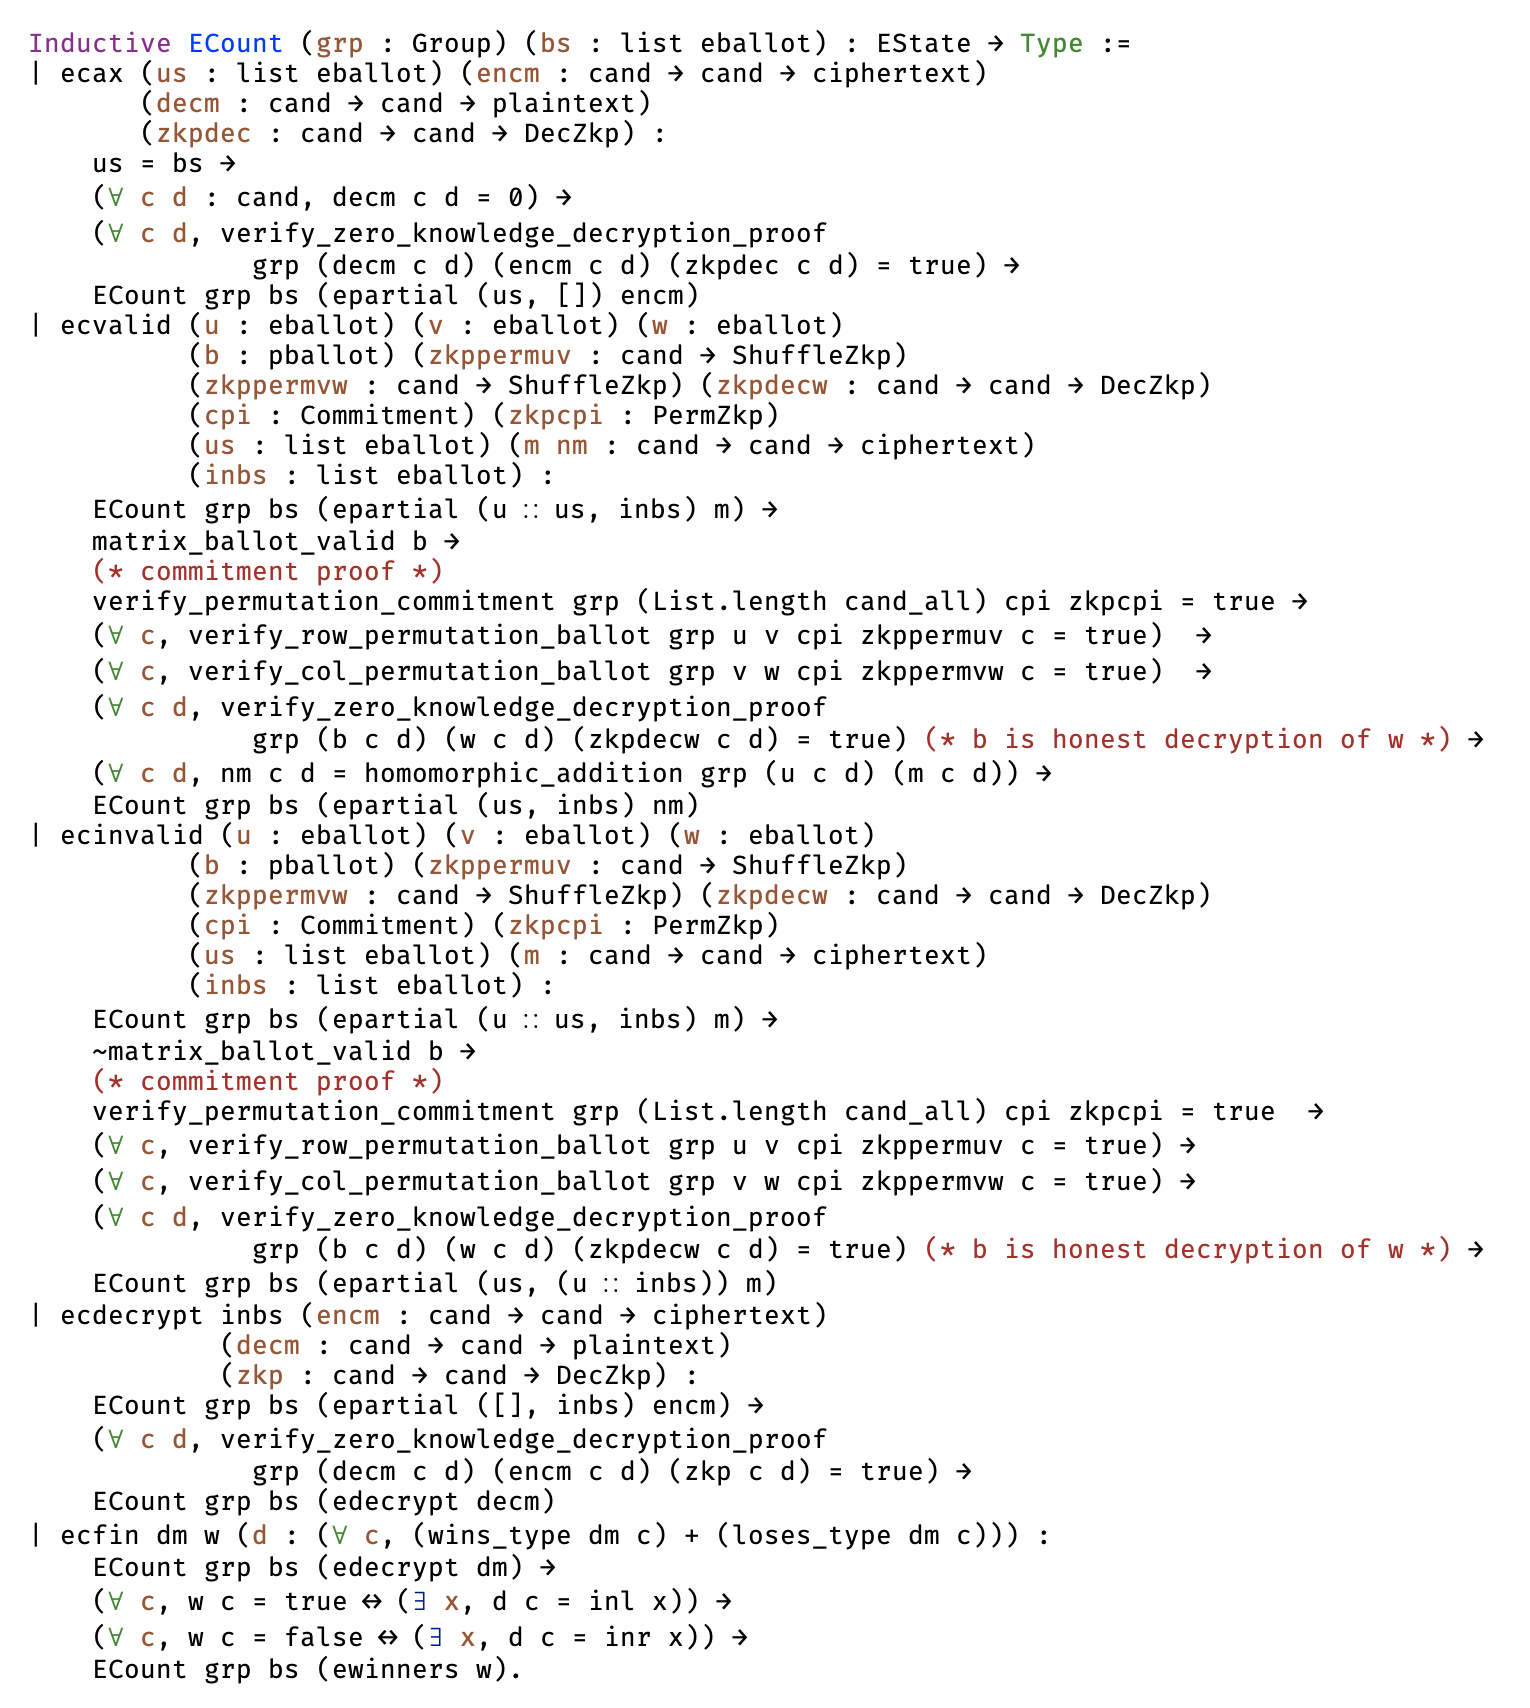
\includegraphics[width=\textwidth]{inductive.png}


\noindent
The constructors of \texttt{EState} then allow us to move from one
state to the next, under appropriate conditions that guarantee
correctness of the count. The different states during the 
counting represented by $ECount$ is tagged by five constructors: 
\begin{itemize}
\item \texttt{ecax}: marks the beginning of counting
\item \texttt{ecvalid}: process a ballot from cast-ballots pile, and the ballot is a valid ballot
\item \texttt{ecinvalid}: process a ballot from cast-ballot pile, and the ballot is a invalid ballot
\item \texttt{ecdecrypt}: decryption of fully constructed homomorphic margin from the cast-ballot
\item \texttt{ecfin}: declaration of winner and loser based on the decrypted margin
\end{itemize}

Inductive type $ECount$ with all the constructors filled with \textit{state data}, 
\textit{verification data}, and \textit{correctness constraint}.  The first constructor, \texttt{ecax}, bootstraps
the count and ensures that 
\begin{itemize}
  \item all ballots are initially uncounted
  \item margin matrix is an encryption of the zero matrix
\end{itemize}

\begin{description}
  \item[state data:] here, the list of uncounted and invalid ballots,
  and the encrypted homomorphic margin
  \item[verification data:] a zero-knowledge proof that the encrypted
  homomorphic margin is indeed an encryption of the zero margin
  \item[correctness constraints:] here, the constructor may only be applied if
  the list of uncounted ballots is equal to the list of ballots
  cast, and the fact that the zero-knowledge proofs indeed verify
  that the initial margin matrix is identically zero.
\end{description}

\noindent
The main difference between the correctness condition, and the
verification data is that the former can be simply be inspected
(here by comparing lists) whereas the latter requires additional
data (here  in the form of a zero-knowledge proof). In Coq, 
this constructor can be encoded as:

\begin{minted}{coq}
 Inductive ECount (grp : Group) (bs : list eballot) : 
  EState -> Type :=
  | ecax (us : list eballot) 
      (encm : cand -> cand -> ciphertext)
      (decm : cand -> cand -> plaintext)
      (zkpdec : cand -> cand -> DecZkp) :
      us = bs ->
      (forall c d : cand, decm c d = 0) -> 
      (forall c d, verify_zero_knowledge_decryption_proof 
          grp (decm c d) (encm c d) (zkpdec c d) = true) ->
    ECount grp bs (epartial (us, []) encm)
\end{minted}



The constructor \texttt{ecvalid} represents the effect of counting a
valid ballot. Here the crucial aspect is that validity needs to be
evidenced. As before, we have:
\begin{description}
  \item[state data:] as before, the list of uncounted and invalid
  ballots, the homomorphic margin, but additionally evidence that
  the previous state has been obtained correctly
  \item[verification data:]
  a commitment to a (secret) permutation, a row permutation of the
  ballot being counted, and a column permutation of this, and a
  decryption of the row- and column permuted ballot (all with
  accompanying zero-knowledge proofs)
  \item[correctness constraints:] all the zero-knowledge proofs
  verify, the new margin is the homomorphic addition of the previous
  margin and the counted ballot, and the decrypted (shuffled)
  ballot is indeed valid. 
\end{description}

\begin{minted}{coq}
  | ecvalid (u : eballot) (v : eballot) (w : eballot)
     (b : pballot) (zkppermuv : cand -> ShuffleZkp)
     (zkppermvw : cand -> ShuffleZkp) 
     (zkpdecw : cand -> cand -> DecZkp)
     (cpi : Commitment) (zkpcpi : PermZkp)
     (us : list eballot) 
     (m nm : cand -> cand -> ciphertext)
     (inbs : list eballot) :
     ECount grp bs (epartial (u :: us, inbs) m) ->
     (* valid ballot *)
     matrix_ballot_valid b ->
     (* commitment proof *)
     verify_permutation_commitment grp 
         (List.length cand_all) cpi zkpcpi = true ->
     (forall c, verify_row_permutation_ballot grp 
         u v cpi zkppermuv c = true)  ->
     (forall c, verify_col_permutation_ballot grp 
         v w cpi zkppermvw c = true)  ->
     (forall c d, verify_zero_knowledge_decryption_proof 
          grp (b c d) (w c d) (zkpdecw c d) = true)  ->
     (forall c d, nm c d = homomorphic_addition
          grp (u c d) (m c d)) -> 
     ECount grp bs (epartial (us, inbs) nm)
       \end{minted}
 
  

The constructor \texttt{ecinvalid}  is very similar to \texttt{ecvalid}.  
We elide the description of the constructor that is applied
when an invalid ballot is being encountered (the only
difference is that the margin matrix is not being updated and ballot is moved to 
list of invalid ballots). 

\begin{minted}{coq}
  | ecinvalid (u : eballot) (v : eballot) (w : eballot)
     (b : pballot) (zkppermuv : cand -> ShuffleZkp)
     (zkppermvw : cand -> ShuffleZkp)
     (zkpdecw : cand -> cand -> DecZkp)
     (cpi : Commitment) (zkpcpi : PermZkp)
     (us : list eballot) (m : cand -> cand -> ciphertext)
     (inbs : list eballot) :
     ECount grp bs (epartial (u :: us, inbs) m) ->
     (* invalid ballot *)
     ~matrix_ballot_valid b ->
     (* commitment proof *)
     verify_permutation_commitment grp
        (List.length cand_all) cpi zkpcpi = true ->
     (forall c, verify_row_permutation_ballot grp
        u v cpi zkppermuv c = true) ->
     (forall c, verify_col_permutation_ballot grp
        v w cpi zkppermvw c = true) ->
     (forall c d, verify_zero_knowledge_decryption_proof 
        grp (b c d) (w c d) (zkpdecw c d) = true) ->
     ECount grp bs (epartial (us, (u :: inbs)) m)
\end{minted}

 

Counting finishes when there are no more uncounted ballots and this state is 
marked by constructor $ecdecrypt$, in
which case the next step is to publish the decrypted margin matrix.
Also here, we have
\begin{description}
  \item[state data:] the decrypted margin matrix, plus evidence
  that a state with no more uncounted ballots has been obtained
  correctly
  \item[verification data:] a zero-knowledge proof that demonstrates
  honest decryption of the final margin matrix
  \item[correctness constraints:] the given zero-knowledge proof
  verifies, i.e. the given decrypted margin is indeed the decryption
  of the (last) homomorphically computed margin matrix.
\end{description} 

 \begin{minted}{coq}
  | ecdecrypt inbs 
      (encm : cand -> cand -> ciphertext)
      (decm : cand -> cand -> plaintext)
      (zkp : cand -> cand -> DecZkp) :
      ECount grp bs (epartial ([], inbs) encm) ->
      (forall c d, verify_zero_knowledge_decryption_proof
          grp (decm c d) (encm c d) (zkp c d) = true) ->
      ECount grp bs (edecrypt decm)
 \end{minted}
 
 
 
 \noindent
The last constructor, $ecfin$, finally declares the winners of the election,
and we have:
\begin{description}
  \item[state data:] a function \texttt{cand -> bool} that determines
  winners, plus evidence of the fact that the decrypted final margin
  matrix has been obtained correctly
  \item[verification data:] 
   paths and co-closed sets that evidence the correctness of the
   function above
 \item[correctness constraints:] that ensure that the verification
 data verifies the winners given by the state data.
\end{description}
This last part is same as the previous chapter's 
scrutiny sheet (section \ref{sec:scrunity_sheet}).

 \begin{minted}{coq}
  | ecfin dm w 
      (d : (forall c, (wins_type dm c) + 
                      (loses_type dm c))) :
      ECount grp bs (edecrypt dm) ->
      (forall c, w c = true <-> (exists x, d c = inl x)) ->
      (forall c, w c = false <-> (exists x, d c = inr x)) ->
      ECount grp bs (ewinners w).  

\end{minted}













\section{Correctness by Construction and Verification}
\label{sec:correct}

In the previous section, we have presented a data type that
\emph{defines} the notion of a verifiably correct count of the
Schulze Method, on the basis of encrypted ballots. To obtain an
executable that in fact \emph{produces} a verifiable (and provably
correct) count, we can proceed in either of two ways:
\begin{enumerate}
  \item implement a function that -- given a list \texttt{bs} of
  ballots -- produces a boolean function \texttt{w} (for winners) and an
  element of the type \texttt{ECount bs (winners w)}. This gives
  both the election winners (\texttt{w}) as well as evidence (the
  element of the \texttt{ECount} data type).
  \item to prove that for every set \texttt{bs} of encrypted
  ballots, we have a boolean function \texttt{w} and an inhabitant
  of the type \texttt{ECount bs (winners w)}.
\end{enumerate}

\noindent
Under the proofs-as-programs interpretation of constructive type
theory, both amount to the same. We chose the latter approach, and
our main theorem formally states that all elections can be
counted according to the Schulze Method (with encrypted ballots),
i.e. a winner can always be found. Formally, our main theorem takes
the following form:
\begin{minted}{coq}
Lemma encryption_schulze_winners (group : Group) 
 (bs : list eballot) : existsT (f : cand -> bool), 
 ECount group bs (ewinners f).
\end{minted}

\noindent
The proof proceeds by successively building an inhabitant of
\texttt{EState} by homomorphically computing the margin matrix, then
decrypting and determining the winners. Within the proof, we use
both generation primitives (e.g. to construct zero-knowledge proofs)
and coherence axioms (to ensure that the zero-knowledge proofs
indeed verify). 

The correctness of our entire approach stands or falls with the
correct formalisation of the inductive data type \texttt{ECount}
that is used to determine the winners of an election counted
according to the Schulze Method. While one can argue that the data
type itself is transparent enough to be its own specification,
the cryptographic aspect makes things slightly more complex. For
example, it appears to be credible that our mechanism for
determining validity of a ballot is correct -- however we have not
given proof of this. Rather than scrutinising the details of the
construction of this data type, we follow a different approach: we
demonstrate that homomorphic counting always yields the same results
as plaintext counting, where plaintext counting is already verified
against its specification (Chapter \ref{cha:schulze_method}). 
This correspondence has two directions, and both assume that we are given
two lists of ballots that are the encryption (resp. decryption) of
one another. 


The first theorem, \texttt{plaintext\_} \texttt{schulze\_to} \texttt{\_homomorphic}, 
reproduced below shows
that every winner that can be determined using plaintext counting
can also be evidenced on the basis of corresponding encrypted ballots. The
converse of this is established by 
Theorem \texttt{homomorphic} \texttt{\_schulze} \texttt{\_to\_plaintext}.

\begin{minted}{coq}
Lemma plaintext_schulze_to_homomorphic 
 (group : Group) (bs : list ballot): 
 forall (pbs : list pballot) (ebs : list eballot) 
 (w : cand -> bool), (pbs = map (fun x => (fun c d => 
 decrypt_message group privatekey (x c d))) ebs) ->
 (mapping_ballot_pballot bs pbs) -> 
 Count bs (winners w) -> ECount group ebs (ewinners w).
      
Lemma homomorphic_schulze_to_plaintext 
 (group : Group) (bs : list ballot):
 forall (pbs : list pballot) (ebs : list eballot) 
 (w : cand -> bool) (pbs = map (fun x => (fun c d => 
 decrypt_message group privatekey (x c d))) ebs) ->
 (mapping_ballot_pballot bs pbs) ->
 ECount grp ebs (ewinners w) -> Count bs (winners w).
\end{minted}

\noindent
The theorems above feature a third type of ballot that is the basis
of plaintext counting, and is a simple ranking function of type
\texttt{cand -> Nat}, and the two hypotheses on the three types of
ballots ensure that the encrypted ballots (\texttt{ebs}) are in fact
in alignment with the rank-ordered ballots (\texttt{bs}) that are
used in plaintext counting. The proof, and indeed the formulation, 
relies on an inductive data
type \texttt{Count}  (Section \ref{sec:inductive_type}) that can best be 
thought of as a plaintext
version of the inductive type  \texttt{ECount} given here.
Crucially, \texttt{Count} is verified against a formal specification
of the Schulze Method. Both theorems are proven by induction on the
definition of the respective data types, where the key step is to
show that the (decrypted) final margins agree. The key ingredient
here are the coherence axioms that stipulate that zero-knowledge
proofs that verify indeed evidence shuffle and/or honest decryption.


\section{Extraction and Experiments} \label{sec:extract}

As discussed in the Section \ref{sec:typeprop}, 
we are using  the Coq extraction
mechanism \citep{Letouzey:2003:NEC}  to extract programs from
existence proofs\footnote{https://github.com/mukeshtiwari/EncryptionSchulze/tree/master/code/Workingcode}.
In particular, we extract the proof of the Theorem
\texttt{pschulze\_winners}, given in Section \ref{sec:correct} to a
program that delivers not only provably correct counts, but also
verifiable evidence.  Give a set of encrypted ballots and a \texttt{Group}
that forms the basis of cryptographic operations, we obtain a program that
delivers not only a set of winners, but additionally independently  verifiable
evidence of the correctness of the count. 

Indeed, the entire formulation of our data type, and the split into
state data, verification data, and correctness constraints, has been
geared towards extraction as a goal. Technically, the verification
conditions are \emph{propositions}, i.e. inhabitants of Type
\emph{Prop} in the terminology of Coq, and hence erased at
extraction time. This corresponds to the fact that the assertions
embodied in the correctness constraints can be verified with minimal
computational overhead, given the state and the verification data.
For example, it can simply be verified whether or not a zero
knowledge proof indeed verifies honest decryption by running
it through a verifier.  On the other hand, the zero-knowledge proof
itself (which is part of the verification data) is crucially needed
to be able to verify that a plaintext is the honest decryption of a
ciphertext, and hence cannot be erased during extraction.
Technically, this is realised by formulating both state and
verification data at type level (rather than as propositions). 

As we have explained in Section \ref{sec:realisation}, the formal
development does not pre-suppose any specific implementation of the
cryptographic primitives, and we assume the existence of
cryptographic infrastructure. From the perspective of extraction,
this produces an executable with ``holes'', i.e. the cryptographic
primitives need to be supplied to fill the holes and indeed be able
to compile and execute the extracted program.  

To fill this hole, we implement the cryptoraphic primitives with
help of the UniCrypt library \citep{LocherH14}.
UniCrypt is a freely available library, written in Java,  that provides nearly all of
the required functionalities, with the exception of honest decryption
zero-knowledge proofs.  We extract our proof development into OCaml
and use Java/OCaml bindings~\citep{OCamlJava} to make the UniCrypt
functionality available to our OCaml program. Due to differences
in the type structure between Java and OCaml, mainly in the context
of sub-typing, this was done in the form of an OCaml wrapper around
Java data structures.  After instantiating the  
 cryptographic primitives in the extracted OCaml code with wrapper
 code that calls UniCrypt,
 we tested the executable on a three candidate elections between
 candidates \texttt{A}, \texttt{B} and \texttt{C}.
 The computation produces a tally sheet that is schematically given
 below:
 it is trace of computation which can be used as a checkable record to verify
 the outcome of election. We elide the cryptographic detail, e.g.
 the concrete representation of zero-knowledge proofs.
 A certificate
 is be obtained from the type \texttt{ECount} where the head
 of the certificate corresponds to the base case of the inductive
 type, here \texttt{ecax}. Below, \texttt{M} is encrypted margin
 matrix, \texttt{D} is its decrypted equivalent, required to be
 identically zero, and \texttt{Z} represents a matrix of zero
 knwoledge proofs, each establishing that the \texttt{XY}-component
 of \texttt{M} is in fact an encryption of zero. All these matrices
 are indexed by candidates and we display these matrices by listing
 their entries prefixed by a pair of candidates, e.g. the ellipsis
 in \texttt{AB(...)} denotes the matrix entry at row \texttt{A} and
 column \texttt{B}.

 {\small
 \begin{verbatim}
 M: AB(rel-marg-of-A-over-B-enc), AC(rel-marg-of-A-over-C-enc), ... 
 D: AB(0)                       , AC(0)                       , ...
 Z: AB(zkp-for-rel-marg-A-B)    , AC(zkp-for-rel-marg-A-C)    , ...
 \end{verbatim}}
 
 \mbox{}\\[-5ex]
 Note that one can verify the fact that the initial encrypted margin
 is in fact the zero margin by just verifying the zero-knowledge
 proofs. Successive entries in the certificate will generally be
 obtained by counting valid, and discarding invalid ballots. If a
 valid ballot is counted after the counting commences, the
 certificate would continue by exhibiting the state and verification
 data contained in the \texttt{ecvalid} constructor which can be
 displayed schematically as follows:

 {\small\begin{verbatim}
 V: AB(ballot-entry-A-B) , AC(ballot-entry-A-C), ...
 C: permutation-commitment
 P: zkp-of-valid-permutation-commitment
 R: AB(row-perm-A-B)     , AC(row-perm-A-C)    , ...
 RP: A(zkp-of-perm-row-A), B(zkp-of-perm-row-B), ... 
 C: AB(col-perm-A-B),      AC(col-perm-A-C)    , ...
 CP: A(zkp-of-perm-col-A), B(zkp-of-perm-col-B), ...
 D: AB(dec-perm-bal-A-B) , AC(dec-perm-bal-A-C), ...
 Z: AB(zkp-for-dec-A-B)  , AC(zkp-for-dec-A-C) , ...
 M: AB(new-marg-A-B)     , AC(new-marg-A-C)    , ...
 \end{verbatim}}

 \mbox{}\\[-5ex]
 Here \texttt{V} is the list of ballots to be counted, where we only
 diplay the first element. We
 commit to a permutation and validate this commitment with a zero
 knowledge proof, here given in the second and third line, prefixed
 with \texttt{C} and \texttt{P}. The following two lines are a row
 permutation of the ballot \texttt{V}, together with a zero
 knowledge proof of correctness of shuffling (of each row) with
 respect to the permutation committed to by \texttt{C} above. The
 following two lines achieve the same for subsequently permuting the
 columns of the (row permuted) ballot. Finally, \texttt{D} is the
 decrypted permuted ballot, and \texttt{Z} a zero-knowledge proof of
 honest decryption. We end with an updated homomorphic margin
 matrix \texttt{M}. Again, we note that the validity of the
 decrypted ballot can be checked easily, and validating zero
 knowledge proofs substantiate that the decrypted ballot is indeed a
 shuffle of the original one. Homomorphic addition can simply be
 re-computed.

 The steps where invalid ballots are being detected are similar, with
 the exception of not updating the margin matrix. Once all ballots
 are counted, the only applicable constructor is \texttt{ecdecrypt},
 the data content of which would continue a certificate
 schematically as follows:

 {\small\begin{verbatim}
 V: []
 M: AB(fin-marg-A-B), AC(fin-marg-A-C), ...
 D: AB(dec-marg-A-B), AC(dec-marg-A-C), ...
 Z: AB(zkp-dec-A-B) , AC(zkp-dec-A-C) , ...
 \end{verbatim}}

 \mbox{}\\[-5ex]
 Here the first line indicates that there are no more ballots to be
 counted, \texttt{M} is the final encrypted margin matrix,
 \texttt{D} is its decryption and \texttt{Z} is a matrix of zero
 knowledge proofs verifying the correctness of decryption.

 The certificate would end with the determination of winners based
 on the encrypted margin, and would end with the content of the
 \texttt{ecfin} constructor

 {\small\begin{verbatim}
 winning: A, <evidence that A wins against B and C>
 losing:  B, <evidence that B loses against A and C>
 losing:  C, <evidence that C loses against A and B>
 \end{verbatim}}

 \mbox{}\\[-5ex]
 where the notion of evidence for winning and losing is as in the
 plaintext version of the protocol (Chapter \ref{cha:schulze_method}).  
 
 \noindent
 \textit{Concrete Certificate:} Below is a glimpse of a concrete certificate for an election. 
We have stripped off 
the trailing digits in the tally sheet which is marked by $..$, and rather 
 than representing an entry of a matrix as ($i$, $j$), it is represented as 
 $ij$

\begin{lstlisting}[frame=none, numbers=none, basicstyle=\ttfamily\scriptsize]

M: AA(13.., 10..) AB(90.., 14..)  AC(11.., 23..) BA(16.., 13..) 
BB(79.., 46..) BC(12.., 14..) CA(50.., 53..) CB(70.., 68..) CC(23.., 82..), 
D: [AA: 0 AB: 0 AC: 0 BA: 0 BB: 0 BC: 0 CA: 0 CB: 0 CC: 0], 
Zero-Knowledge-Proof-of-Honest-Decryption: [..]
------------------------------------------------------------------------------
V: [AA(42.., 15..) AB(63.., 32..) AC(70, 44..) BA(47.., 34..) BB(16.., 28..)
BC(39.., 16..) CA(19.., 13..) CB(57.., 12..) CC(19.., 89..),..], I:  [], 
M: AA(12.., 11..) AB(13.., 66..) AC(16.., 14.) BA(48.., 31..) BB(15.., 52..)
BC(15.., 68..) CA(39.., 69..) CB(12.., 78..) CC(10.., 40..),
Row-Permuted-Ballot: AA(53.., 16..) AB(23.., 44..) AC(72.., 47..) 
BA(10.., 19..) BB(74.., 16..) BC(20.., 60..) CA(44.., 10..) CB(12.., 16..)
CC(59.., 98..),
Column-Permuted-Ballot: AA(81.., 41..) AB(17.., 14..) AC(10.., 14..) 
BA(37.., 12..) BB(14.., 66..) BC(10.., 13..) CA(12.., 13..) CB(14.., 16..)
CC(12.., 10..),
Decryption-of-Permuted Ballot: AA0 AB-1 AC1 BA1 BB0 BC1 CA-1 CB-1 CC0,
Zero-Knowledge-Proof-of-Row-Permutation: [Tuple[...]], 
Zero-Knowledge-Proof-of-Column-Permutation: [Tuple[..]], 
Zero-Knowledge-Proof-of-Decryption: [Triple[..]], 
Permutation-Commitment: Triple[..]
Zero-Knowledge-Proof-of-Commitment: Tuple[..]
------------------------------------------------------------------------------
.
.
.
------------------------------------------------------------------------------
V: [AA(36.., 10..) AB(20.., 13..) AC(75.., 43..) BA(13.., 31..) BB(27.., 82..)
BC(31.., 50..) CA(16.., 11..) CB(74.., 15..) CC(26.., 36..)], I: [],
M: AA(86.., 38..) AB(21.., 14..) AC(16.., 25..) BA(16.., 22..) BB(18.., 15..)
BC(11.., 63..) CA(15.., 34..) CB(76.., 18..) CC(11.., 10..), 
Row-Permuted-Ballot: .., Column-Permuted-Ballot: .., 
Decryption-of-Permuted-Ballot: AA0 AB-10 AC1 BA10 BB0 BC1 CA-1 CB-1 CC0,
Zero-Knowledge-Proof-of-Row-Permutation: [..],
Zero-Knowledge-Proof-of-Column-Permutation: [..], 
Zero-Knowledge-Proof-of-Decryption: [..], 
Permutation-Commitment: Triple[..], 
Zero-Knowledge-Proof-of-Commitment: Tuple[..]
------------------------------------------------------------------------------
V: [], I: [AA(36.., 10..) AB(20.., 13..) AC(75.., 43..) BA(13.., 31..) 
BB(27.., 82..) BC(31.., 50..) CA(16.., 11..) CB(74.., 15..) CC(26.., 36..)], 
M: .., D: [AA: 0 AB: 4 AC: 4 BA: -4 BB: 0 BC: 4 CA: -4 CB: -4 CC: 0],
Zero-Knowledge-Proof-of-Decryption: [..]
------------------------------------------------------------------------------
D: [AA: 0 AB: 4 AC: 4 BA: -4 BB: 0 BC: 4 CA: -4 CB: -4 CC: 0]
winning: A
   for B: path A --> B of strength 4, 5-coclosed set: 
       [(B,A),(C,A),(C,B)]
   for C: path A --> C of strength 4, 5-coclosed set:
       [(B,A),(C,A),(C,B)] 
losing: B
   exists A: path A --> B of strength 4, 4-coclosed set: 
     [(A,A),(B,A),(B,B),(C,A),(C,B),(C,C)]
losing: C
   exists A: path A --> C of strength 4, 4-coclosed set: 
     [(A,A),(B,A),(B,B),(C,A),(C,B),(C,C)]

\end{lstlisting}


\begin{figure}
\centering
%\vspace*{-1cm}
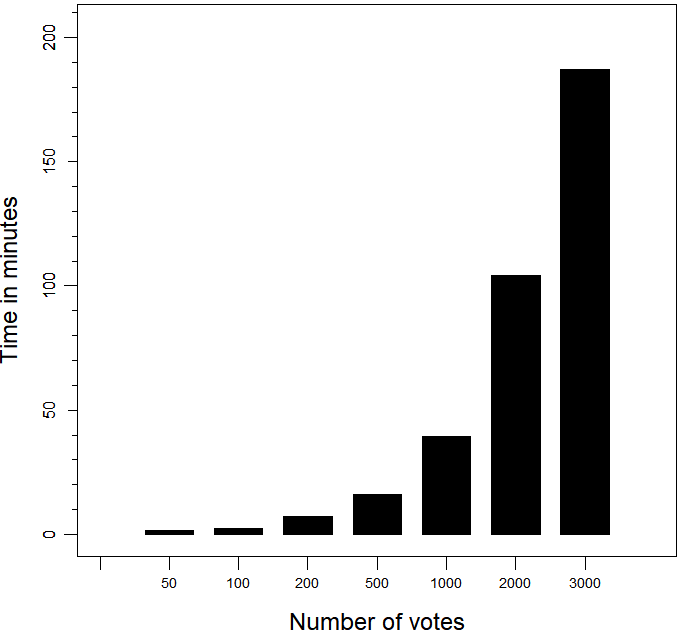
\includegraphics[scale=0.80]{PlotVer3.png}
\caption{Experimental Result}
  \label{fig:experimental_result}
\end{figure}
 We note that the schematic presentation of the certificate above is
 nothing but a representation of the data contained in the extracted
 type \texttt{ECount} that we have chosen to present schematically.
 Concrete certificates can be inspected with the accompanying proof
 development, and are obtained by simply implementing datatype to
 string conversion on the type \texttt{ECount}.
 



To demonstrate proof of concept, 
we have run our experiment on an  Intel  i7  2.6  GHz  Linux  desktop  computer
with  16GB  of  RAM for three candidates and randomly generated ballots (Figure \ref{fig:experimental_result}). 
The largest  amount of ballot we counted was 10,000 (not included in
graph), with a runtime of 25 hours. A more detailed analysis reveals
that the bottleneck are the bindings between OCaml and Java. More
specifically, producing the cryptographic evidence using the
UniCrypt Library for 10,000 ballots takes about 10 minutes, and the
subsequent computation (which is the same as for the plaintext
count) takes negligible time. This is consistent with the mechanism
employed by the bindings:
each function call from OCaml to Java is inherently memory bounded
and creates an instance of the Java runtime, 
the conversion of OCaml data structures into Java data
structures, 
computation by respective Java function producing result,
converting the result back into OCaml data structure, and finally destroying 
the Java runtime instance when the function returns. While the proof
of concept using OCaml/Java bindings falls short of being
practically feasible, our timing analysis substantiates that
feasibility can be achieved by eliminating the overhead of the
bindings. 


\section{Summary}
\label{sec:summary_homomorphic}

\noindent The main contribution of our formalisation is that of independently
verifiable \emph{evidence} for a set of candidates to be the winners
of an election counted according to the Schulze method. Our main
claim is that our notion of evidence is both safeguarding the
privacy of the individual ballot (as the count is based on encrypted
ballots) and is verifiable at the same time (by means of zero
knowledge proofs). To do this, we have axiomatised a set of
cryptographic primitives to deal with encryption, decryption,
correctness of shuffles and correctness of decryption. From formal
and constructive proof of the fact that such evidence can always be
obtained, we have then extracted executable code that is provably
correct by construction and produces election winners together with
evidence once implementations for the cryptographic primitives are
supplied.

In a second step, we have supplied an implementation of these
primitives, largely based on the UniCrypt Library. Our experiments
have demonstrated that this approach is feasible, but quite clearly
much work is still needed to improve efficiency. 

\smallskip\noindent\emph{Assumptions for Provable Correctness.}
While we claim that the end product embodies a high level of
reliability, our approach necessarily leaves some gaps between the
executable and the formal proofs. First and foremost, this is of
course the implementation of the cryptographic primitives in an
external (and unverified) library. We have minimised this gap by
basing our implementation on a purpose-specific existing library
(UniCrypt) to which we relegate most of the functionality. 


\smallskip\noindent\emph{Modelling Assumptions.} In our modelling of
the cryptographic primitives, in particular the zero-knowledge
proofs, we assumed properties which in reality only hold with
very high probability. As a
consequence our correctness assertions only hold to the level
of probability that is guaranteed by zero-knowledge proofs (Sigma 
protocols).

\smallskip\noindent\emph{Scalability.} We have analysed the
feasibility of the extracted code by counting an increasing number
of ballots. While this demonstrates a proof of concept, our results
show that the bindings used to couple the cryptographic layer with
our code adds significant overhead compared
to plaintext tallying in Schulze method (\ref{cha:schulze_method}).  Given that both
parts are practically efficient by themselves, scalability is merely
the question of engineering a more efficient coupling. 


In a nutshell, the achieved and failed parts of this formalization:

\begin{itemize}
\item Achieved
\begin{itemize}
\item Correctness: The implementation is formalized in Coq assuming the 
         existence of cryptographic 
         functions and axioms about their correctness behaviour. These primitives were 
         used for constructing evidence, or certificate. 
         
\item Privacy : We don't reveal the content of ballot at any phase of election counting. Therefore, 
         there is no possibility of anyone knowing the choices of a voter other than the voter herself.
                 
\item Verifiability: The outcome of any election can be verified by any third party because 
          of the generated certificates. However,
          the nature of certificates in this case is very complex and can only be scrutinize 
          by someone having specialized knowledge of cryptography which decreases the pool of potential 
          scrutinizers dramatically.

\end{itemize}
\item Failed
\begin{itemize}
 \item Correctness: We use an external unverified library for cryptographic code.  In general, this library 
 		  could have bugs and 
          may produce a wrong result. This is not a problem per say because it will be caught during the 
          certificate checking by any independent party, but it may create a atmosphere of distrust among 
          voters.  
 
 
\end{itemize}
\end{itemize}


\noindent
Our formalization leaves some gaps which needs to be filled:
\begin{itemize}
\item A formally verified cryptographic library to fill the \textit{correctness gap}.
\item A formally verified checker to ease the auditing of election to fill the \textit{scrutineers} gap
\end{itemize}


Developing a formally verified library to fill the correctness gap would have taken more time,
specifically the commitment consistent shuffle, 
so we chose to formally verify the certificate checker to ease the auditing of election to 
increase the number of scrutineers gap. 
 
In the next chapter, we will focus on all the details needed to 
develop formally verified certificate checker for the certificate we produced in this chapter. 
However, we did not 
formalize every cryptographic primitive needed to verify our certificate. Rather, 
we have developed a proof of concept formally verified certificate checker for 
 International Association for Cryptologic Research 2018 election, a simpler 
 scrutiny sheet than ours which does not involve any shuffle. 

\chapter{Scrutiny Sheet : Software Independence}
\label{cha:software_independence}
\setlength{\parindent}{2em}

\epigraph{Somewhere inside of all of us is the power to change the world.} 
{\textit{Roald Dahl }}

\section{Introduction}


A major disadvantage of using cryptography 
to achieve privacy,  using encryption to make the 
content of ballot private, and verifiability, using zero-knowledge proof for verification of claims,
is that the verification process  is quite cumbersome. As a consequence, the verification process 
(checking the scrutiny sheet) is only viable for
cryptographers,  a tiny fraction of general population,  and results into 
a sharp decrease in number of scrutineers. 
While it is not very difficult to find cryptographers to verify the election, 
they are, off course, not the representative population in any democracy. 
In order to increase the number of scrutineers and subsequently confidence in electronic voting, we follow the 
route of providing a formally verified open-source 
reference certificate checker which anyone can inspect and run on the election data. 
  The rationale behind formally verifying the certificate checker is \emph{correctness}
  and open sourcing is to gain the public trust  via careful examination.  
  For example, consider a scenario where we do not provide the reference checker,
  then how 
  likely would it be for community/voters to develop the 
  verified checker? Moreover, assuming that we publish one unverified certificate checker,
  what would happen if it returns false on a valid certificate because of its own bug? 
  Both situations, of course, would be a devastating situation, so not only 
  should we provide a reference certificate checker, but it should be a formally verified one. 
  Additionally, a formally verified reference certificate checker would open the gate for
  debate in case of someone's implementation for checking certificate diverges from the reference checker.
In the case of a diverging situation, there are two possibilities, either the reference checker is verified 
using wrong assumptions,  or the implementation itself is wrong.  The first situation is certainly 
not very pleasant because it would deteriorate the public trust in the system, but nonetheless, it is always
good to  have openness in democracy to make it more strong. 
 

\textbf{Contribution:} We examine the concepts needed to develop a formally 
verified scrutiny sheet checker,  produced from the encrypted ballots in the previous chapter. 
Most of these concepts, except the shuffle proof, are straight forward and easy to implement,  so
we formally verify these easy concepts in Coq to develop a certificate 
checker for another election, which uses simple method to elect candidates. 

In this chapter, we discuss the concepts required to develop a verified certificate checker for the certificate we generated 
in the last chapter.  Moreover, we sketch pseudo code and pen-and-paper proof, in style of algebraic manipulation.  
 The reason for doing this to make
it accessible for everyone who intends to develop a formally verified certificate checker.  
In some cases, we have translated the pseudo code in Coq code to make the idea more precise. 


We have already explained our certificate in section \ref{sec:extract}, 
but intuitively,  checking our certificate amounts to proving that  the homomorphic margin has been 
computed correctly and zero-knowledge proof for every claim is correct. In a nutshell, 
our claims were:
\begin{enumerate}
\item honest decryption zero-knowledge proof: every encrypted value is decrypted honestly 
\item shuffle zero-knowledge proof:
  a ballot has been permuted by the same permutation whose commitment is published (commitment consistent shuffle \citep{Wikstrom:2009:CPS}).
\item final homomorphic tally is computed correctly
\end{enumerate}


\noindent
We sketch the encoding of Pedersen's commitment \citep{Pederson}, one of the primitives of shuffle zero-knowledge proof, in Coq, 
but we leave the other details of shuffle zero-knowledge proof algorithm \citep{Wikstrom:2009:CPS}. Moreover, we
encode the sigma protocol in Coq as a record and give various examples of concrete sigma protocol, including 
the honest decryption zero-knowledge proof.   We also describe the computation of homomorphic tally from the encrypted 
ballots, without decryption any individual ballot.  Finally, all 
these concepts are sufficient to develop the formally verified 
certificate checker for International Association for Cryptologic Research (IACR) election\footnote{\url{https://vote.heliosvoting.org/helios/elections/60a714ea-ce6d-11e8-8248-76b4ab96574c/view}}
because IACR uses a very simple method, compared to ours, to elect candidates,  
and our proof development can be accessed\footnote{\url{https://github.com/mukeshtiwari/secure-e-voting-with-coq}}. 

\textbf{Chapter Outline:} In section $\ref{sec:algebra}$, we discuss the underlying algebraic structures needed for various 
 cryptographic operations. Section $\ref{sec:pedersen}$ focuses on generalizing the Pedersen commitment scheme for 
 a matrix. In the following section $\ref{sec:sigma_coq}$, we discuss the details of sigma protocol, and its formalization 
 in Coq. In order to eschew the (monadic) probabilistic reasoning of sigma protocol, we use the standard trick of making the randomness 
 explicit to make the reasoning easier
 without losing the meaning of sigma protocol. In section $\ref{sec:conc_sigma}$, we show 
 how to make a concrete instance of sigma protocol by giving an example of discrete logarithm. In addition, 
 we show the protocol needed for honest decryption (section $\ref{sec:dec_sigma}$). Section $\ref{sec:homo_tally}$ sketches 
 the homomorphically tally based on additive ElGamal scheme. Finally, we discuss the IACR scrutiny sheet in section $\ref{sec:election_iacr}$, 
 and we summarize the chapter in section $\ref{sec:summary_software}$


\section{Algebraic Structures: Building Blocks}
\label{sec:algebra}
The basic building blocks of any cryptographic system are algebraic structures, specifically cyclic group (of prime order), field, and vector space. In general, 
we do not need vector space, and group and field are sufficient for most of the cryptographic purposes. However,
vector space  of a cyclic group of prime order over the field of integers (vector element) modulo the same field of integers of same prime order (scalar element)
is nicer to work because the operation involving an element from group and an element from field can be abstracted over 
the scalar multiplication operator of vector space.   For example,  in elliptic curve cryptography,  for a given curve $E$ over a finite field,   
there are two main operations: i) point-addition (adding two points $P$ and $Q$, given of the curve $E$),  and ii) point-multiplication (multiplying a field element, 
$a$, with a point, $P$, on the curve $E$).  Moreover,  there is also a point at infinity (denoted by $O$) which acts as an identity element.   
We can easily implement these functions using the suitable data-structure from the Coq theorem prover and prove theorems about them.  
Nonetheless,  during the process of proving these theorems a lot of details about 
the internal implementation of these functions would make it unnecessarily complicated\footnote{it is more likely to be the case that some key lemma required would be missing from the library,  
and it will some effort to prove it}, while if we abstract the point-addition and   point-multiplication as  vector-addition and scalar-multiplication, respectively, 
of a vector space, we can prove theorems about these functions,   point-addition and  point-multiplication, using just axioms of vector space.  
The proof process would be much smoother,  but more importantly, the proof would just require the axioms of vector space and field.
This was the major motivation behind abstracting the group and field over a vector space.  Now we briefly explain the group, field, and vector space. 

\begin{definition}[Group] 
A group is a set $G$, with a binary operator $\cdot : G \rightarrow G \rightarrow G$, identity element $e$, and inverse operator $inv : G \rightarrow G$ (denoted as $^{-1}$) such 
    that the following laws hold:  \end{definition} 
    \begin{itemize}
     \item \textit{Associativity}: $\forall \text{  }a \text{  }b \text{  }c \text{  } \in G,$  $a \cdot (b \cdot c) = (a \cdot b) \cdot c$
    \item \textit{Closure}: $\forall \text{  } a \text{  } b \text{  } \in G,$  $a \cdot b \in G$
    \item \textit{Inverse Element}: $\forall \text{  } a \text{  } \in G$, $a \cdot \text{ } a^{-1} = \text{ } a^{-1} \cdot a = e$
    \item \textit{Identity}: $\forall \text{  } a \text{  } \in G,$  $a \cdot e = e \cdot a  = a$
    \end{itemize}
  
    \noindent
    If the group is commutative, i.e. $\forall \text{  } a \text{  }b \text{  }\in  G, \text{   } a \cdot b = b \cdot a$, then we call it Abelian group.  We can represent the Abelian group in Coq by using the 
    record data type. 
 
 \begin{minted}{Coq}

Record AbelGroup (G : Type)
    (dot : G -> G -> G)  (inv : G -> G) (e : G) :=
  {
    dot_associativity : forall x y z, 
      dot x (dot y z) = dot (dot x y) z;
    dot_left : forall x, dot x e = x;
    dot_right : forall x, dot e x = x;
    left_inverse : forall x, dot (inv x) x = e;
    right_inverse : forall x, dot x (inv x) = e;
    commutative : forall x y, dot x y = dot y x
  }.
  
\end{minted}

\noindent
Our Coq encoding is slight different from the definition of the group we gave above, mainly that \textit{G : Type} (read as G has the type Type). 
Because of the underlying foundation of Coq is type theory, every term in Coq has a type;
hence we need to explicitly state the type of term $G$.  In a nutshell, Type is used to represent set.  

\begin{definition}[Field] 
A field  is a set $\mathbb{F}$, with two binary operators $+ : \mathbb{F} \rightarrow \mathbb{F} \rightarrow \mathbb{F}$,  and $\cdot : \mathbb{F} \rightarrow \mathbb{F} \rightarrow \mathbb{F}$, 
two identity elements $0$ and $1$, and two unary operator $- : \mathbb{F} \rightarrow \mathbb{F}$, $1/ : \mathbb{F} \rightarrow \mathbb{F}$  such that:
\end{definition} 
 \begin{itemize}
 \item ($\mathbb{F}$, +, 0, -) forms an abelian group.
 \item ($\mathbb{F}$ - $\lbrace 0 \rbrace$, $\cdot$, 1, 1/) forms an abelian group.
 \item $\cdot$ distributes over +.
 \end{itemize}
 
 

\begin{definition}[Vector Space]
A set $V$ with two binary operations,  vector addition $+ : V \rightarrow V \rightarrow V$  and scalar multiplication $\cdot : \mathbb{F}  \rightarrow V \rightarrow V$, 
is  a vector space over a field $\mathbb{F}$ if the following properties hold:
\end{definition} 
\begin{itemize}
 \item Closure under vector addition: (V, +) forms an abelian group. 
 \item Scalar multiplication distributes  with respect  to  vector  addition: $\forall$  $r \in \mathbb{F}$, $u$ $v$ $\in V$,  $r \cdot (u + v) = r \cdot u + r \cdot v$.
 \item Scalar multiplication distributes with respect to field addition: 
                $\forall$  $a$ $b$ $\in \mathbb{F}$, $u$ $\in V$, $(a +_{\mathbb{F}} b) \cdot u = a \cdot u + b \cdot v$, where $+_{\mathbb{F}} : \mathbb{F} \to \mathbb{F} \to \mathbb{F} $ is 
                field addition. 
  \item Scalar multiplication is associative with respect to field multiplication:
         $\forall$ $a$ $b$ $\in  \mathbb{F}$, $u$ $\in V$ , $(a \cdot_{\mathbb{F}} b) \cdot u = a \cdot (b \cdot u)$, where $\cdot_{\mathbb{F}} : \mathbb{F} \to \mathbb{F} \to \mathbb{F} $ is 
                field  multiplication. 
  \item Identity: $\forall a \in V, 1_{\mathbb{F}} \cdot a = a$

\end{itemize}



\section{Pedersen Commitment Scheme}
\label{sec:pedersen}
Recall that in the last chapter to prove that if a ballot was valid or invalid, we generated a secret permutation $\pi$ and published its commitment using 
Pedersen commitment scheme \citep{Pederson}.  Later, we use this to shuffle each row and column of the ballot by this (secret) permutation. 
In the shuffle algorithm \citep{Wikstrom:2009:CPS}), the data structure of permutation $\pi$ is matrix (a permutation matrix to be precise).
In this section, we discuss that how to generalized Pedersen commitment scheme for matrix data structure. 

A Pedersen commitment for any two given group elements $g$ $h$ $\in G$, a message $m \in \mathbb{F}$ (the field of integers), and a random element 
$r \in \mathbb{F}$ (the field of integers) is $g^r \cdot h^m$ ($\cdot$ is the group operation).   
As we explained above that we can just work with group and field, but abstracting the group operation ($\cdot : G \to G \to G$) as 
a vector-addition and exponentiation operation ($\textasciicircum :  G \to \mathbb{F} \to G$) as scalar-multiplication would make the 
proofs more tractable.  Finally we can encode the Pedersen commitment in the Coq 
theorem prover (simplified for the presentation):

\begin{minted}{coq}

Definition ped_commitment {F G : Type} (H1 : Group G) 
	(H2 : Field F) (H3 : Vector_Space F G) 
	(^ : G -> F -> G) (dot : G -> G -> G) 
	(g h : G) (r m : F) : G :=  dot (g ^ r) (h ^ m).

\end{minted}

\noindent
The Coq definition of Pedersen commitment assumes the existence of two types
$F$ and $G$, together with hypothesis that $G$ is group, $F$ is field, and  
both, $F$ and $G$, forms a vector space (we are not giving any concrete implementation of group or field, 
but an abstract representation, assuming two abstract type $G$ and $F$.  During the code extraction,  we instantiate all 
these types and operations with a concrete representation and discharge the proof 
obligation to make sure that the assumptions hold, very similar to the Schulze algorithm 
extraction where we instantiate the $Cand$ type with concrete candidates 
and discharge all the proof obligation).


We can extend the Pedersen commitment to commit a vector instead of 
just a scalar.  To commit a
vector of $n$ group elements $h_{1}, h_{2} \dots h_{n}$, vector of $n$ 
field elements $m_{1}, m_{2} \dots m_{n}$,  a group element $g$,  and a random field element 
$r$,  we compute  $g^r \cdot \prod_{i = 1}^n  h_{i}^{m_{i}}$.  This commitment is 
known as vector Pedersen commitment.  
The $\prod_{i = 1}^n  h_{i}^{m_{i}}$ can be computed in Coq as 
(this program is written using Equation library \citep{Sozeau:2019:ERH:3352468.3341690}):

\begin{minted}{coq}


Equations prod_vh_commitment  {F G : Type} {n : nat} 
	(H1 : Group G) (H2 : Field F)
	(H3 : Vector_Space F G)  (^ : G -> F -> G) 
	(dot : G -> G -> G) (hi : Vector.t G (S n)) 
	(mi : Vector.t F (S n)) :  G :=
prod_vh_commitment (^) dot (vcons h vnil) (vcons m vnil) := 
	h ^ m;
prod_vh_commitment (^) dot (vcons h hs)  (vcons m ms)  := 
	dot (h ^ m) (prod_vh_commitment ^ dot hs ms).


\end{minted}

\noindent
Now we can compute the vector Pedersen commitment ($g^r \cdot  \prod_{i = 1}^n  h_{i}^{m_{i}}$) as:

\begin{minted}{coq}

Definition ped_vec_commitment {F G : Type} {n : nat} 
	(H1 : Group G) (H2 : Field F)
	(H3 : Vector_Space F G)  (^ : G -> F -> G)
	(g : G) (r : F) (hs : Vector.t G (n + 1))
	(ms : Vector.t F (n + 1)) := 
	dot (g ^ r) 
	(prod_vh_commitment H1 H2 H3 ^ dot hs ms)  
\end{minted}
  
 
\noindent
Finally,  we can extend the idea of vector Pedersen commitment to commit a matrix of size  $N \times N$,  for some arbitrary natural number $N$.
To do so, we can call the $ped\_vec\_commitment$ on every column of the matrix.   Consequently, 
we  will get a vector of commitments of length $N$.



\section{Sigma Protocol: Efficient Zero-Knowledge Proof}
\label{sec:sigma_coq}
A sigma protocol is a two party protocol, a prover $P$ and a verified $V$, where prover $P$ tries to convince the verifier $V$ that she 
holds a private input $x$ for some public input $w$ such that a binary relation $R$ holds, i.e. $(x, w) \in R$.  Sigma protocol, 
in general, is a three step protocol:
\begin{enumerate}
\item Initialisation: $P$ generates a random challenge $r$, commits it, and sends the committed message to $V$
\item Challenge: $V$ generates a random challenge $e$ and sends it to $V$
\item Response: $P$ sends a response $z$ to $V$
\end{enumerate} 

\noindent
Finally, upon receiving the response $z$ and other public inputs, $V$ 
either accepts the proof or rejects the proof,  depending on if the public inputs are consistent with protocol or not.  The verification step is 
modelled as a boolean function that takes all the public inputs and returns true or false.  
Now we define the sigma protocol in Coq by using record data type.

\begin{minted}{coq}
Record SigmaProtocol (Statement : Type) (* Statement x *)
       (Witness : Type) (* witness w *)
       (R : Statement -> Witness -> bool) (* decidable relation *)
       (RandCoin : Type) (* random coin *) 
       (Commitment : Type) (* commitments *)
       (Challenge : Type) (* challenges *) 
       (Response : Type) (* response *) :=
  MkSigma {
  (* initial commitment send by the Prover *)
  initial : RandCoin -> Commitment;
  (* Randomness send by the verifier.  *) 
  challenge : Challenge;
  (* response generate by prover *)
  response : Statement -> Witness ->
     RandCoin -> Challenge ->
     Response;
  (* verify the response *)
  verify : Statement * Commitment * Challenge * Response
  -> bool;
  (* Simulator *)
  simulator : Statement -> Challenge -> Response ->
     Statement * Commitment * Challenge * Response;
  (* Extractor *)
  extractor : Challenge -> Response -> Challenge -> 
     Response -> Witness;
  

  (* Completness *)
  Completness : forall (s : Statement) (w : Witness)
    (r : RandCoin) (e : Challenge),  R s w = true -> 
    verify (s, initial r, e, response s w r e) = true;

 (* Special Soundness *)
  Special_Soundness : forall s c e1 e2 r1 r2,
    e1 <> e2 ->
    verify (s, c, e1, r1) = true ->
    verify (s, c, e2, r2) = true ->
    R s (extractor e1 r1 e2 r2) = true;
  
 (* Special honest verifier zero knowledge proof. Explicit 
    randomness makes it nicer to work in theorem prover  *)
  Special_Honest_Verifier_ZKP  (s : Statement) 
    (w : Witness) (e : Challenge): 
    R s w = true -> forall (r : RandCoin), 
    verify (s, initial r, e, response s w r e) = true <->
    forall (z : Response), verify (simulator s e z) = true;
  
 (* simulator correct *)
  Simulator_correct : forall (s : Statement) 
   (e : Challenge) (r : Response),
   verify (simulator s e r) = true;
  }.
\end{minted}


\noindent
The record \textit{SigmaProtocol} is indexed by:
\begin{itemize}
\item $Statement$, the public input known to $P$ and $V$
\item $Witness$, secret input known to $P$
\item $R$ such that $(x, w) \in R$, known to $P$ and $V$
\item $RandCoin$, the private random coin toss of $P$
\item $Commitment$, commitment computed by $P$ based on the random coin toss
\item $Challenge$, the random challenge of $V$ to $P$
\item $Response$, the response of $P$ send to $V$
\end{itemize}

\noindent
The body of record SigmaProtocol contains
functions $initia$,  $challenge$, and $response$
to reflect the three steps of sigma protocol with three auxiliary 
functions  and $verify$,  $simulator$, and $extractor$.  
The  $verify$, a boolean  function, checks if the data produced 
during the protocol is consistent or not, $simulator$ function produces 
a transcript and used for proving the special honest verifier zero knowledge proof, 
and $extractor$ function produces a witness  and used in special soundness of 
sigma protocol. 

\noindent
We have four correctness properties about sigma protocol:
\begin{enumerate}
\item $Completeness:$ if $P$ and $V$ follow the protocol, then 
verifier would accept the proof. 
\item $Special\_Soundness:$ if $P$ is able to convince $V$ with two 
accepting transcript for the same commitment, then $V$ can extract the witness.
\item $Special\_Honest\_Verifier\_ZKP:$ recall that  special honest 
verifier zero knowledge proof amounts to a probabilistic polynomial time simulator 
$S$ which would generate a proof transcript for some statement 
$s$  with same probability distribution as if there were a real 
conversation between a prover $P$ and a verifier $V$ 
for the statement $s$ and witness $w$ such that $(s, w) \in  R$.
Informally, the real proof transcript depends on statement $s$, witness $w$,  
and challenge $e$,  while the simulated proof transcript depends on statement $s$ and challenge $e$. 
(simulator does have not access to witness $w$, so to generate a accepting 
proof just by using $s$ and $e$, it uses a concept call rewinding.)
In our definition of $Special\_Honest\_Verifier\_ZKP$, we eschew the 
probabilistic reasoning by making randomness explicit, and it
states that for any  given 
fixed statement $s$, witness $w$, challenge $e$ and assumption that $R$ $s$ $w$ holds, 
then for every random challenge $r$  and a accepting real transcript, simulator can construct 
an accepting transcript from all random responses drawn from response space. 
\item $Simulator\_correct:$ simulator is correct,  i.e. any transcript created by simulator checks out. 

\end{enumerate}
 


Finally, we can use our construction,  $SigmaProtocol$, as a building block 
for composing different kinds of sigma protocols, which we are not explaining 
here.  For example,  we can define AND composition, EQ composition, OR composition, etc.

\subsection{Concrete Sigma Protocol: Discrete Logarithm}
\label{sec:conc_sigma}
One of the most basic sigma protocol is proof of knowledge of 
discrete logarithm, i.e. given two elements $g$ and $h$ of 
a group $G$, prover convinces the verifier that 
she knows the discrete logarithm ($\log_g h$) in zero 
knowledge. In Camenisch-Stadler notation \citep{camenisch1997proof} of zero knowledge proof, it is represented as:
$ZKPoK \lbrace w \text{ | } h = g^w \rbrace$. We can show 
that this is a sigma protocol inside Coq
by encoding all the  functions 
and proving all the axioms mentioned in 
our record type $SigmaProtocol$.  For example,
 we can write the $initial$ function as taking a input $r$ 
 and computing 
$g^r$, $challenge$ as a function which simply returns 
a challenge $e$, and so forth: 


\begin{displayquote}

$\text{initial g r := } g^r$  

$\text{challenge := } e$

$\text{response h w r e := } r + e \cdot w$

$\text{verify g h a e z  := } g^z = a \cdot h^e$

$\text{simulator g h s e z := } (g^z \cdot h^{-e}, e, z)$

$\text{extractor }  $c_{1}$ $z_{1}$ $c_{2}$ $z_{2}$ := (z_{1} - z_{2}) \cdot (c_{2} - c_{1})^{-1}$

\end{displayquote}

Based on these definitions, we can easily discharge the three proofs,  $Completeness$, 
$Special\_Soundness$,  $Special\_Honest\_Verifier\_Zero\_Knowledge$, and $Simulator\_correct$ axioms by simple 
algebraic manipulation.

\subsection{Honest Decryption Zero Knowledge Proof}
\label{sec:dec_sigma}
We have sigma protocol at our arsenal, we focus on honest decryption 
problem. How can we convince someone that for a given group 
$(G, g, p, h)$ and private key $x$ ($h := g^x$), the message $m$ is the 
honest decryption of ElGamal ciphertext $(c_{1}, c_{2})$ (which is $(g^r, g^m \cdot h^r)$ for some randomness $r$
with revealing 
our private key $x$? To solve this problem, we use a well known protocol
for proving equality of the discrete logarithm \citep{10.1007/3-540-69053-0_9}.
We first discuss the protocol, and later we will show that how we can adopt 
the protocol for our purpose. 

\textbf{Diffie Hellman Tuple:} a tuple $(g, h, u, v)$ is 
 a Diffie Hellman  tuple if there exists a $w$ such that 
 $u = g^w$ and $v = h^w$.  The protocol to prove it is:
 
 \begin{itemize}
 \item $P$ chooses a random $r$ and sends $a=g^r$ and $b = h^r$.
 \item $V$ sends a random $e$
 \item $P$ sends $z =r+ e \cdot w$
 \item $V$ check $g^z = a \cdot u^e$ and $h^z = b\cdot v^e$ 
 \end{itemize}
 

Now we come back to our original problem, i.e. proving that $m$ is the honest 
decryption of $(c_{1}, c_{2})$. From these values, we construct a Diffie Hellman tuple
by multiplying $c_{2}$ with $g^{-m}$, i.e.
$(g, h, c_{1}, c_{2} \cdot g^{-m})$. A simple algebraic simplification shows that 
this tuple can be written as $(g, h, g^r, g^m \cdot h^r \cdot g^{-m})$ for some 
random $r$. A further simplification leads to $(g, h, g^r, h^r)$, and 
this tuple is clearly a Diffie Hellman tuple, where $u = g^r$ and $v = h^r$. 
We could not have been able to construct a  Diffie Hellman tuple and proved 
the equality of discrete logarithm if we had claimed anything other than the origin value $m$. For example, 
suppose a cheating prover  claims that $m_{1}$ (different from $m$) is the honest decryption of $(c_{1}, c_{2})$.
Following the cheating prover claim, we construct the Diffie Hellman tuple 
 $(g, h, g^r, g^{m} \cdot h^r \cdot g^{-m_{1}})$. 
 Clearly, the tuple $(g, h, g^r, h^r \cdot g^{m - m_{1}})$ is not 
Diffie Hellman tuple; hence a cheating prover would not succeed. 




\section{Homomorphic Tally}
\label{sec:homo_tally}
Now that we have sorted out the correct decryption, the next challenge in our 
tally sheet is  computing the final tally homomorphically.  Since our encryption 
is additive ElGamal, and recall that our ballot is a matrix of ciphertexts: 

\begin{pmatrix}
  (g^{r_{11}}, g^{m_{11}} * h^{r_{11}})&  (g^{r_{12}}, g^{m_{12}} * h^{r_{12}}) & \cdots &  (g^{r_{1N}}, g^{m_{1N}} * h^{r_{1N}}) \\
 (g^{r_{21}}, g^{m_{21}} * h^{r_{21}})&  (g^{r_{22}}, g^{m_{22}} * h^{r_{22}}) & \cdots &  (g^{r_{2N}}, g^{m_{2N}} * h^{r_{2N}}) \\
  \vdots  & \vdots  & \ddots & \vdots  \\
  (g^{r_{N1}}, g^{m_{N1}} * h^{r_{N1}})&  (g^{r_{N2}}, g^{m_{N2}} * h^{r_{N2}}) & \cdots &  (g^{r_{NN}}, g^{m_{NN}} * h^{r_{NN}}) \\
 \end{pmatrix}


To compute the finally tally, all we have to do is to stack all the valid
ballots (matrices) together and multiply the corresponding ciphertexts 
together to get the final tally matrix (point wise matrix multiplication). 
The final computed tally can be 
decrypted honestly by using the same principals described in the previous 
section.  We can capture all these concepts in Coq based on the 
algebraic structures, group, field, vector space, and prove all the 
properties by simple algebraic manipulation. We can represent 
encryption, decryption and ciphertext multiplication for 
a given cyclic group $(G, g, h, x)$ such that $h = g^x$:

\begin{displayquote}
$\text{elGamal\_enc (g h : G) (r : F) :=} (g^r, g^m \cdot h^r)$

$\text{elGamal\_dec (g h : G) }  (c_{1}, c_{2}) := c_{2} \cdot c_{1}^{-x}$

$\text{elGamal\_mult } (c_{1}, c_{2}) (d_{1}, d_{2}) := (c_{1} \cdot d_{1}, c_{2} \cdot d_{2})$

\end{displayquote}

\noindent
In fact, by simple algebraic manipulation, we can prove that 
decryption is left inverse of encryption. 


\begin{align}
  \text{elGamal\_dec g h (elGamal\_enc g h r)} &= \text{elGamal\_dec g h } (g^r, g^m \cdot h^r)  (unfolding) \nonumber \\
                     &= g^m \cdot h^r \cdot (g^r)^{-x}  (unfolding) \nonumber \\
                     &= g^m \cdot (g^x)^r \cdot (g^r)^{-x} (substitution) \nonumber \\
                     &=  g^m \cdot g^{xr} \cdot g^{-rx} (algebraic-simplification)\nonumber \\
                     &= g^m\nonumber 
\end{align}


\noindent 
The final decrypted tally would be a matrix filled with values like $g^{m_{1} + m_{2} + \cdots }$, and we 
need to do a search to find the values of $m_{1} + m_{2} + \cdots$ from the 
final decrypted tally. A drawback of this method is that if the number of candidates and ballots are
 large, then calculating $m_{1} + m_{2} + \cdots$ from 
	      $g^{m_{1} + m_{2} + \dotsb  + m_{n}}$ is 
	      not very practical \citep{10.1007/3-540-69053-0_9}.  


\section{IACR 2018 Election}
\label{sec:election_iacr}
We follow some of these techniques explained above to write a formal 
certificate checker for  IACR 2018 directors election scrutiny sheet
\footnote{\url{https://vote.heliosvoting.org/helios/elections/60a714ea-ce6d-11e8-8248-76b4ab96574c/view}}.  
The 2018  IACR directors election considered seven 
 candidates to fill three positions on the board of directors.   The voting 
 style is approval voting where all the eligible voters, IACR members, 
 could vote for as many candidates as they like. After the counting, 
 the top three members were elected to fill the positions. 
 
The Helios voting system \citep{Helios:2016:HVS}  was used for the election, and the system
was configured with four authorities, who generated an ElGamal \citep{elgamal1985public}  public
key such that all four authorities were required to decrypt efficiently.    
Every eligible voter received the credentials by email which they used 
to cast their ballot from their personal computer. 
During the cast process, each voter created seven ElGamal ciphertexts, 
encrypting either zero or one, for the seven participating candidates. 
Since the vote was exponent, the ElGamal cryptosystem became 
homomorphic additive.  During this point,  the voter was then offered the chance to audit 
her encrypted ballot to check that
it indeed had the vote of her choice. If she chose to audit,  she had to
discard this ballot and asked to cast 
a fresh ballot (this mechanism is called called Benaloh challenge, 
and the purpose of this challenge is to catch "cheating machines". 
Moreover, this method ensures the cast-as-intended because 
a cheating machine would not know when a voter would 
cast her ballot, so, in the most likely scenario, a voter would 
end up cast her true intentions).  Once she had an 
unaudited ballot with which she was happy,  she cast it. 
The Helios website maintained an append-only bulletin board on which the voter's
encrypted ballot appeared.  
After the voting period was over,
all the encrypted ballots corresponding to all candidates were multiplied together; so that there was 
a single ciphertext for each candidate, encoding the number of votes for
that candidate.  The authorities then decrypted 
these (seven) ciphertexts, announced the result and proved,
using a sigma protocol, that the announced result was the 
correct decryption.


Now that we have already explained the workings of IACR 2018 directors election,
we focus on 
three aspects of verifiability: cast-as-intended, collected-as-cast, 
and tallied-as-collected.  
The cast-as-intended has already been assured 
by Benaloh challenges, and collect-as-cast is ensured by every voter 
checking her ballot on the bulletin board. 
The more complicated step is the tallied-as-cast
check.  In order to verify the tallied-as-cast, a scrutineer has to check 
only the valid ballots (those which are encryption of either zero or one) 
has contributed to final tally, the final tally has been calculated 
correctly, and the final tally has been decrypted honestly. 

The algorithm, in more detail,  to ascertain the tallied-as-cast, 
there is a published list of encrypted ballots on the bulletin board
and a published result.  Moreover, to enable scrutiny, the election authority publishes, 
non-interactive, sigma protocol transcripts for correct encryption and decryption. 
Using these transcripts,  the scrutineer can verify the election by checking the following
three things. First, all the ballots included in final tally are indeed the encryption of 
zero or one, and any ballot containing any other value has been discarded. 
Second, the scrutineer reruns the (multiplication)
computation and checks that the resulting ciphertexts matches the published one.
Finally, she checks that the transcripts are valid for the decryption of these
combined ciphertexts with respect to the announced result.  These  three checks
suffice to ensure that the ballots were counted-as-collected. 


IACR used Schnorr group \citep{10.1007/0-387-34805-0_22} to avoid attacks various attacks on solving the discrete 
logarithm problem.  A Schnorr group is a multiplicative Abelian subgroup of prime order q of the field of 
integers modulo a prime p, where p = k * q + 1 for some integer.   In IACR election, 
the primes used were:
\begin{minted}[fontsize=\footnotesize]{coq}

Definition P : Z := 16328632084933010002384055033805457329601614771
1859553897391673090862148004064657990385836349537529416756455621824
9812075026498049238137557936767564877129380031037096474576701424363
8518442553823973482995267304044326777047662957480269391322789378384
6194285964464469846943061876447674624609656225800875643392126317758
1789595840901667639897567126617963789855768731707617721884323315069
5157881061257053019133078545928983562221396313169622475509818442661
0470184362648069010239662367183672047107559358990137503061077380023
6413791742659573740387111418775080434656473125060919684663818390398
2387884578266136503697493474682071.


Definition Q : Z := 61329566248342901292543872769978950870633559608
669337131139375508370458778917.


\end{minted}

Since theorem provers are known for proving mathematical statements, but not for being good at running 
computation inside their environment. Naturally, proving any mathematical statement, e.g. number 
theoretic proofs, which are computational intensive would not be a ideal situation for theorem provers. 
However, the recent advancement in theorem provers (specifically Coq) led
us to prove primality of two large prime numbers inside the Coq.
To begin with we utilise the CoqPrime
library\footnote{https://github.com/thery/coqprime} to prove in Coq that the
numbers used to define the Schnorr group are
in fact prime.
\begin{minted}{coq}

Lemma P_prime : prime P.

Lemma Q_prime : prime Q.

\end{minted}


Finally, we extract the OCaml code from Coq proof scripts and write a main file to glue the 
extracted code and parsing code. Upon execution, the code returns 
yes, which asserts that the results produced are correct. 


\section{Summary}
\label{sec:summary_software}
In this chapter, we have sketched the ideas for developing a formally verified certificate checker
for the certificate we produced in the last chapter. However, due to time constraint and 
complexity of shuffle primitive, 
we ended up verifying a simple certification, which did not involve any zero-knowledge proof 
of shuffle.  Finally, in this chapter we closed the loop of decrease in number of scrutineers because 
any one can run the certificate checker. Moreover, we open sourced 
\footnote{\url{https://github.com/mukeshtiwari/secure-e-voting-with-coq}} the checker, so 
that it can be inspected by anyone (we would like to call it correctness by democratic 
process).  One thing we would like to emphasize that cryptographic concepts are 
inherently very complex, so running a certificate checker certainly does not amounts 
to understanding the various bits of cryptography and formal method used to develop the
certificate checker.

In the next chapter, we will discuss some of the properties of Schulze method which we have 
formalized in Coq. 











































   
   
   
   
   
   
\chapter{Machine Checked Schulze Properties}
\label{cha:machine_checked}
 There are various criteria on which we measure the voting scheme. It was not until the pioneer Arrow who proved 
 that a preferential voting scheme can not have all the properties (Arrow Paradox). 
 
 
 Schulze method comes very close to fulling many criteria set by voting experts; however, 
 it can not full fill all because of Arrow paradox. In  
 
 \section{Properties}
	 List some properties which it follows with pictures ?
 	\subsection{Condercet Winner}
 	\subsection{Reversal Symmetry}
 	\subsection{Monotonicity}
 	\subsection{Schwartz set}
\chapter{Conclusion}
\label{cha:conc}
Summary your thesis and discuss what you are going to do in the future in Section~\ref{sec:future}.


\section{Future Work}
\label{sec:future}
Good luck.





%%%%%%%%%%%%%%%%%%%%%%%%%%%%%%%%%%%%%%%%%%%%%%%%%%%%%%%%%%%%%%%%%%%%%%
% Here begins the end matter

%%% \appendix

\backmatter

\bibliographystyle{anuthesis}
\bibliography{thesis}

\printindex

\end{document}
